\documentclass[]{book}
\usepackage{lmodern}
\usepackage{amssymb,amsmath}
\usepackage{ifxetex,ifluatex}
\usepackage{fixltx2e} % provides \textsubscript
\ifnum 0\ifxetex 1\fi\ifluatex 1\fi=0 % if pdftex
  \usepackage[T1]{fontenc}
  \usepackage[utf8]{inputenc}
\else % if luatex or xelatex
  \ifxetex
    \usepackage{mathspec}
  \else
    \usepackage{fontspec}
  \fi
  \defaultfontfeatures{Ligatures=TeX,Scale=MatchLowercase}
\fi
% use upquote if available, for straight quotes in verbatim environments
\IfFileExists{upquote.sty}{\usepackage{upquote}}{}
% use microtype if available
\IfFileExists{microtype.sty}{%
\usepackage{microtype}
\UseMicrotypeSet[protrusion]{basicmath} % disable protrusion for tt fonts
}{}
\usepackage[margin=1in]{geometry}
\usepackage{hyperref}
\PassOptionsToPackage{usenames,dvipsnames}{color} % color is loaded by hyperref
\hypersetup{unicode=true,
            pdftitle={HealthyR: R for healthcare data analysis},
            pdfauthor={Riinu ots and Ewen Harrison},
            colorlinks=true,
            linkcolor=Maroon,
            citecolor=Blue,
            urlcolor=Blue,
            breaklinks=true}
\urlstyle{same}  % don't use monospace font for urls
\usepackage{natbib}
\bibliographystyle{apalike}
\usepackage{color}
\usepackage{fancyvrb}
\newcommand{\VerbBar}{|}
\newcommand{\VERB}{\Verb[commandchars=\\\{\}]}
\DefineVerbatimEnvironment{Highlighting}{Verbatim}{commandchars=\\\{\}}
% Add ',fontsize=\small' for more characters per line
\usepackage{framed}
\definecolor{shadecolor}{RGB}{248,248,248}
\newenvironment{Shaded}{\begin{snugshade}}{\end{snugshade}}
\newcommand{\KeywordTok}[1]{\textcolor[rgb]{0.13,0.29,0.53}{\textbf{#1}}}
\newcommand{\DataTypeTok}[1]{\textcolor[rgb]{0.13,0.29,0.53}{#1}}
\newcommand{\DecValTok}[1]{\textcolor[rgb]{0.00,0.00,0.81}{#1}}
\newcommand{\BaseNTok}[1]{\textcolor[rgb]{0.00,0.00,0.81}{#1}}
\newcommand{\FloatTok}[1]{\textcolor[rgb]{0.00,0.00,0.81}{#1}}
\newcommand{\ConstantTok}[1]{\textcolor[rgb]{0.00,0.00,0.00}{#1}}
\newcommand{\CharTok}[1]{\textcolor[rgb]{0.31,0.60,0.02}{#1}}
\newcommand{\SpecialCharTok}[1]{\textcolor[rgb]{0.00,0.00,0.00}{#1}}
\newcommand{\StringTok}[1]{\textcolor[rgb]{0.31,0.60,0.02}{#1}}
\newcommand{\VerbatimStringTok}[1]{\textcolor[rgb]{0.31,0.60,0.02}{#1}}
\newcommand{\SpecialStringTok}[1]{\textcolor[rgb]{0.31,0.60,0.02}{#1}}
\newcommand{\ImportTok}[1]{#1}
\newcommand{\CommentTok}[1]{\textcolor[rgb]{0.56,0.35,0.01}{\textit{#1}}}
\newcommand{\DocumentationTok}[1]{\textcolor[rgb]{0.56,0.35,0.01}{\textbf{\textit{#1}}}}
\newcommand{\AnnotationTok}[1]{\textcolor[rgb]{0.56,0.35,0.01}{\textbf{\textit{#1}}}}
\newcommand{\CommentVarTok}[1]{\textcolor[rgb]{0.56,0.35,0.01}{\textbf{\textit{#1}}}}
\newcommand{\OtherTok}[1]{\textcolor[rgb]{0.56,0.35,0.01}{#1}}
\newcommand{\FunctionTok}[1]{\textcolor[rgb]{0.00,0.00,0.00}{#1}}
\newcommand{\VariableTok}[1]{\textcolor[rgb]{0.00,0.00,0.00}{#1}}
\newcommand{\ControlFlowTok}[1]{\textcolor[rgb]{0.13,0.29,0.53}{\textbf{#1}}}
\newcommand{\OperatorTok}[1]{\textcolor[rgb]{0.81,0.36,0.00}{\textbf{#1}}}
\newcommand{\BuiltInTok}[1]{#1}
\newcommand{\ExtensionTok}[1]{#1}
\newcommand{\PreprocessorTok}[1]{\textcolor[rgb]{0.56,0.35,0.01}{\textit{#1}}}
\newcommand{\AttributeTok}[1]{\textcolor[rgb]{0.77,0.63,0.00}{#1}}
\newcommand{\RegionMarkerTok}[1]{#1}
\newcommand{\InformationTok}[1]{\textcolor[rgb]{0.56,0.35,0.01}{\textbf{\textit{#1}}}}
\newcommand{\WarningTok}[1]{\textcolor[rgb]{0.56,0.35,0.01}{\textbf{\textit{#1}}}}
\newcommand{\AlertTok}[1]{\textcolor[rgb]{0.94,0.16,0.16}{#1}}
\newcommand{\ErrorTok}[1]{\textcolor[rgb]{0.64,0.00,0.00}{\textbf{#1}}}
\newcommand{\NormalTok}[1]{#1}
\usepackage{longtable,booktabs}
\usepackage{graphicx,grffile}
\makeatletter
\def\maxwidth{\ifdim\Gin@nat@width>\linewidth\linewidth\else\Gin@nat@width\fi}
\def\maxheight{\ifdim\Gin@nat@height>\textheight\textheight\else\Gin@nat@height\fi}
\makeatother
% Scale images if necessary, so that they will not overflow the page
% margins by default, and it is still possible to overwrite the defaults
% using explicit options in \includegraphics[width, height, ...]{}
\setkeys{Gin}{width=\maxwidth,height=\maxheight,keepaspectratio}
\IfFileExists{parskip.sty}{%
\usepackage{parskip}
}{% else
\setlength{\parindent}{0pt}
\setlength{\parskip}{6pt plus 2pt minus 1pt}
}
\setlength{\emergencystretch}{3em}  % prevent overfull lines
\providecommand{\tightlist}{%
  \setlength{\itemsep}{0pt}\setlength{\parskip}{0pt}}
\setcounter{secnumdepth}{5}
% Redefines (sub)paragraphs to behave more like sections
\ifx\paragraph\undefined\else
\let\oldparagraph\paragraph
\renewcommand{\paragraph}[1]{\oldparagraph{#1}\mbox{}}
\fi
\ifx\subparagraph\undefined\else
\let\oldsubparagraph\subparagraph
\renewcommand{\subparagraph}[1]{\oldsubparagraph{#1}\mbox{}}
\fi

%%% Use protect on footnotes to avoid problems with footnotes in titles
\let\rmarkdownfootnote\footnote%
\def\footnote{\protect\rmarkdownfootnote}

%%% Change title format to be more compact
\usepackage{titling}

% Create subtitle command for use in maketitle
\newcommand{\subtitle}[1]{
  \posttitle{
    \begin{center}\large#1\end{center}
    }
}

\setlength{\droptitle}{-2em}
  \title{HealthyR: R for healthcare data analysis}
  \pretitle{\vspace{\droptitle}\centering\huge}
  \posttitle{\par}
  \author{Riinu ots and Ewen Harrison}
  \preauthor{\centering\large\emph}
  \postauthor{\par}
  \predate{\centering\large\emph}
  \postdate{\par}
  \date{2018-01-30}

\usepackage[utf8]{inputenc}
\usepackage{booktabs}
\usepackage{amsthm}
\makeatletter
\def\thm@space@setup{%
  \thm@preskip=8pt plus 2pt minus 4pt
  \thm@postskip=\thm@preskip
}
\makeatother


%%%%%%%%%%%%%%%%
% stuff copied from https://github.com/rstudio/bookdown/blob/master/inst/examples/latex/preamble.tex
% to make the custom blocks

\usepackage{framed,color}
\definecolor{shadecolor}{RGB}{248,248,248}

\renewcommand{\textfraction}{0.05}
\renewcommand{\topfraction}{0.8}
\renewcommand{\bottomfraction}{0.8}
\renewcommand{\floatpagefraction}{0.75}

\renewenvironment{quote}{\begin{VF}}{\end{VF}}
\let\oldhref\href
\renewcommand{\href}[2]{#2\footnote{\url{#1}}}

\ifxetex
  \usepackage{letltxmacro}
  \setlength{\XeTeXLinkMargin}{1pt}
  \LetLtxMacro\SavedIncludeGraphics\includegraphics
  \def\includegraphics#1#{% #1 catches optional stuff (star/opt. arg.)
    \IncludeGraphicsAux{#1}%
  }%
  \newcommand*{\IncludeGraphicsAux}[2]{%
    \XeTeXLinkBox{%
      \SavedIncludeGraphics#1{#2}%
    }%
  }%
\fi

\makeatletter
\newenvironment{kframe}{%
\medskip{}
\setlength{\fboxsep}{.8em}
 \def\at@end@of@kframe{}%
 \ifinner\ifhmode%
  \def\at@end@of@kframe{\end{minipage}}%
  \begin{minipage}{\columnwidth}%
 \fi\fi%
 \def\FrameCommand##1{\hskip\@totalleftmargin \hskip-\fboxsep
 \colorbox{shadecolor}{##1}\hskip-\fboxsep
     % There is no \\@totalrightmargin, so:
     \hskip-\linewidth \hskip-\@totalleftmargin \hskip\columnwidth}%
 \MakeFramed {\advance\hsize-\width
   \@totalleftmargin\z@ \linewidth\hsize
   \@setminipage}}%
 {\par\unskip\endMakeFramed%
 \at@end@of@kframe}
\makeatother


\renewenvironment{Shaded}{\begin{kframe}}{\end{kframe}}


\newenvironment{rmdblock}[1]
  {
  \begin{itemize}
  \renewcommand{\labelitemi}{
    \raisebox{-.7\height}[0pt][0pt]{
      {\setkeys{Gin}{width=3em,keepaspectratio}\includegraphics{images/#1}}
    }
  }
  \setlength{\fboxsep}{1em}
  \begin{kframe}
  \item
  }
  {
  \end{kframe}
  \end{itemize}
  }


\newenvironment{healthyr}
  {\begin{rmdblock}{cover}}
  {\end{rmdblock}}

\newenvironment{warning}
  {\begin{rmdblock}{warning}}
  {\end{rmdblock}}

\newenvironment{error}
  {\begin{rmdblock}{error}}
  {\end{rmdblock}}

% end custom blocks definitions
%%%%%%%%%%%%%%%%

\begin{document}
\maketitle

{
\hypersetup{linkcolor=black}
\setcounter{tocdepth}{1}
\tableofcontents
}
\chapter*{Preface}\label{preface}
\addcontentsline{toc}{chapter}{Preface}


\includegraphics[width=50.35in]{images/cover}

Version 0.3.

Contributors: Riinu Ots, Ewen Harrison, Tom Drake, Peter Hall, Kenneth
McLean.

This work is licensed under the Creative Commons
Attribution-NonCommercial-NoDerivs 3.0 United States License. To view a
copy of this license, visit
\url{http://creativecommons.org/licenses/by-nc-nd/3.0/us/}

\section{Installation}\label{installation}

\begin{healthyr}
\begin{itemize}
\tightlist
\item
  Download R
\end{itemize}
\end{healthyr}

\url{https://www.r-project.org/}

\begin{healthyr}
\begin{itemize}
\tightlist
\item
  Install RStudio
\end{itemize}
\end{healthyr}

\url{https://www.rstudio.com/products/rstudio/}

\begin{healthyr}
\begin{itemize}
\tightlist
\item
  Install packages (copy these lines into the Console in RStudio):
\end{itemize}
\end{healthyr}

\begin{Shaded}
\begin{Highlighting}[]
\KeywordTok{install.packages}\NormalTok{(}\StringTok{"tidyverse"}\NormalTok{)}

\KeywordTok{install.packages}\NormalTok{(}\StringTok{"gapminder"}\NormalTok{)}

\KeywordTok{install.packages}\NormalTok{(}\StringTok{"gmodels"}\NormalTok{)}

\KeywordTok{install.packages}\NormalTok{(}\StringTok{"Hmisc"}\NormalTok{)}

\KeywordTok{install.packages}\NormalTok{(}\StringTok{"devtools"}\NormalTok{)}

\NormalTok{devtools}\OperatorTok{::}\KeywordTok{install_github}\NormalTok{(}\StringTok{"ewenharrison/summarizer"}\NormalTok{)}

\KeywordTok{install.packages}\NormalTok{(}\StringTok{"pROC"}\NormalTok{)}

\KeywordTok{install.packages}\NormalTok{(}\StringTok{"survminer"}\NormalTok{)}
\end{Highlighting}
\end{Shaded}

\begin{warning}
When working with data, don't copy or type code directly into the
Console. We will only be using the Console for viewing output, warnings,
and errors (and installing packages as in the previous section). All
code should be in a script and executed (=Run) using Control+Enter (line
or section) or Control+Shift+Enter (whole script). Make sure you are
always working in a project (the right-top corner of your RStudio
interface should say ``HealthyR'').
\end{warning}

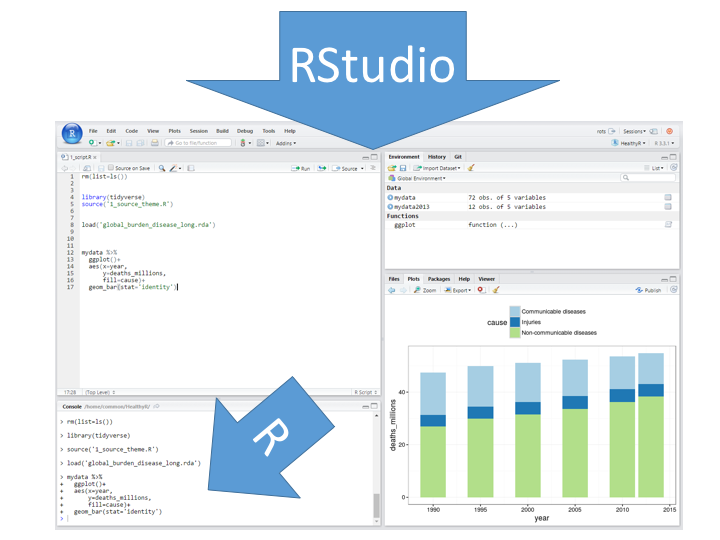
\includegraphics[width=10in]{images/rstudio_vs_r}

\section{Datasets}\label{datasets}

\begin{healthyr}
Files:

gbp.rda

gbp.csv

melaoma\_factored
\end{healthyr}

\begin{error}
These will include common errors.
\end{error}

\chapter*{(PART*) Part I: Always plot your data
first}\label{part-part-i-always-plot-your-data-first}
\addcontentsline{toc}{chapter}{(PART*) Part I: Always plot your data
first}

\chapter{Your first R plots}\label{your-first-r-plots}

In this session, we will create 5 beautiful and colourful barplots in
less than an hour. Do not worry about understanding every single word or
symbol (e.g.~the pipe - \texttt{\%\textgreater{}\%}) in the R code you
are about to see. The purpose of this session is merely to

\begin{itemize}
\tightlist
\item
  gain familiarity with the RStudio interface:

  \begin{itemize}
  \tightlist
  \item
    to know what a script looks like,
  \item
    what is the Environment tab,
  \item
    where do your plots appear.
  \end{itemize}
\end{itemize}

\section{Data}\label{data}

Load the example dataset which is already saved as an R-Data file
(recognisable by the file extension .rda/.RData):

\begin{Shaded}
\begin{Highlighting}[]
\KeywordTok{library}\NormalTok{(ggplot2)}

\KeywordTok{source}\NormalTok{(}\StringTok{"1_source_theme.R"}\NormalTok{)}

\KeywordTok{load}\NormalTok{(}\StringTok{"global_burden_disease_long.rda"}\NormalTok{)}
\CommentTok{#loads two dataframes - mydata and mydata2013 which is a subset of mydata}
\end{Highlighting}
\end{Shaded}

After loading the datasets, investigate your Environment tab
(top-right):

Click on the name \texttt{mydata} and it will pop up next to where your
script is. Clicking on the blue button is not as useful, but it doesn't
do any harm either. Try it.

\section{First plot}\label{first-plot}

\begin{Shaded}
\begin{Highlighting}[]
\NormalTok{mydata }\OperatorTok\StringTok{ }\CommentTok{#press Control-Shift-M to insert this symbol (pipe)}
\StringTok{  }\KeywordTok{ggplot}\NormalTok{(}\KeywordTok{aes}\NormalTok{(}\DataTypeTok{x      =}\NormalTok{ year,}
             \DataTypeTok{y      =}\NormalTok{ deaths_millions,}
             \DataTypeTok{fill   =}\NormalTok{ cause,}
             \DataTypeTok{colour =}\NormalTok{ cause)) }\OperatorTok{+}
\StringTok{  }\KeywordTok{geom_col}\NormalTok{()}
\end{Highlighting}
\end{Shaded}

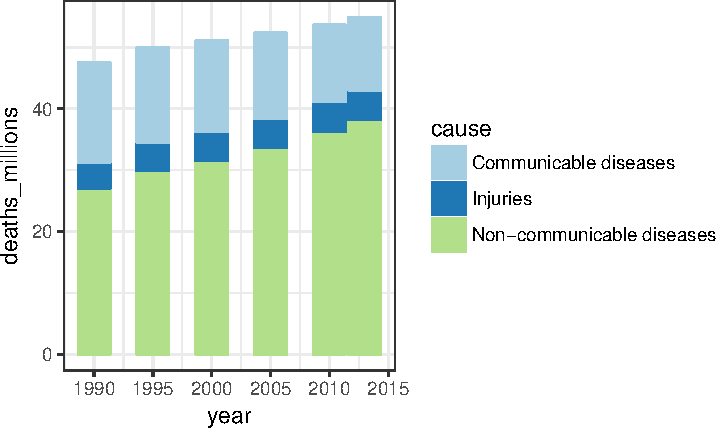
\includegraphics{01_first_interaction_files/figure-latex/unnamed-chunk-2-1.pdf}

\texttt{ggplot()} stands for \textbf{grammar of graphics plot} - a user
friendly yet flexible alternative to \texttt{plot()}.

\texttt{aes()} stands for \textbf{aesthetics} - things we can see.

\texttt{geom\_()} stands for \textbf{geometric}.

\subsection{Question}\label{question}

Why are there two closing brackets - \texttt{))} - after the last
aesthetic (colour)?

\subsection{Exercise}\label{exercise}

Plot the number of deaths in Developed and Developing countries for the
year 2013:

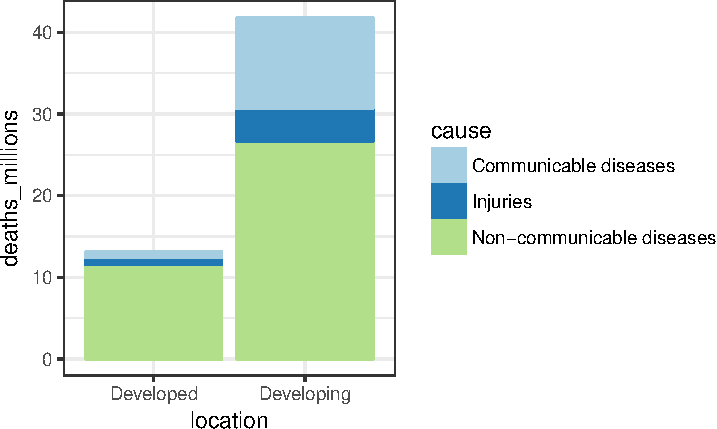
\includegraphics{01_first_interaction_files/figure-latex/unnamed-chunk-3-1.pdf}

\newpage

\section{Comparing bars of different
height}\label{comparing-bars-of-different-height}

\subsection{Stretch each bar to 100\%}\label{stretch-each-bar-to-100}

\texttt{position="fill"} stretches the bars to show relative
contributions:

\begin{Shaded}
\begin{Highlighting}[]
\NormalTok{mydata2013 }\OperatorTok\StringTok{ }
\StringTok{  }\KeywordTok{ggplot}\NormalTok{(}\KeywordTok{aes}\NormalTok{(}\DataTypeTok{x      =}\NormalTok{ location,}
             \DataTypeTok{y      =}\NormalTok{ deaths_millions,}
             \DataTypeTok{fill   =}\NormalTok{ cause,}
             \DataTypeTok{colour =}\NormalTok{ cause)) }\OperatorTok{+}
\StringTok{  }\KeywordTok{geom_col}\NormalTok{(}\DataTypeTok{position =} \StringTok{"fill"}\NormalTok{)}
\end{Highlighting}
\end{Shaded}

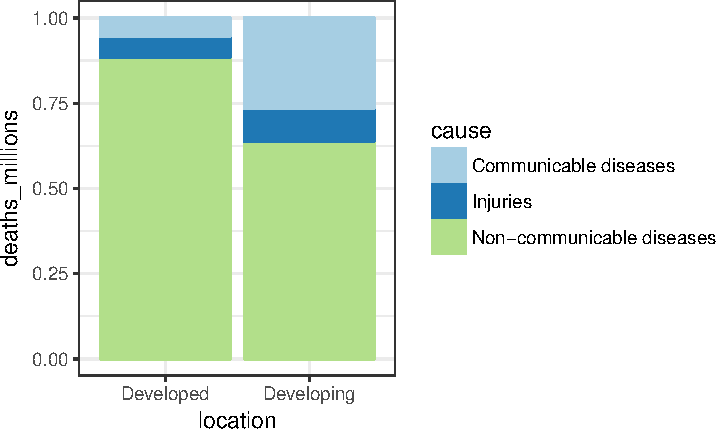
\includegraphics{01_first_interaction_files/figure-latex/unnamed-chunk-4-1.pdf}

\subsection{Plot each bar next to each
other}\label{plot-each-bar-next-to-each-other}

\texttt{position="dodge"} puts the different causes next to each rather
(the default is \texttt{position="stack"}):

\begin{Shaded}
\begin{Highlighting}[]
\NormalTok{mydata2013 }\OperatorTok\StringTok{ }
\StringTok{  }\KeywordTok{ggplot}\NormalTok{(}\KeywordTok{aes}\NormalTok{(}\DataTypeTok{x      =}\NormalTok{ location,}
             \DataTypeTok{y      =}\NormalTok{ deaths_millions,}
             \DataTypeTok{fill   =}\NormalTok{ cause,}
             \DataTypeTok{colour =}\NormalTok{ cause)) }\OperatorTok{+}
\StringTok{  }\KeywordTok{geom_col}\NormalTok{(}\DataTypeTok{position =} \StringTok{"dodge"}\NormalTok{)}
\end{Highlighting}
\end{Shaded}

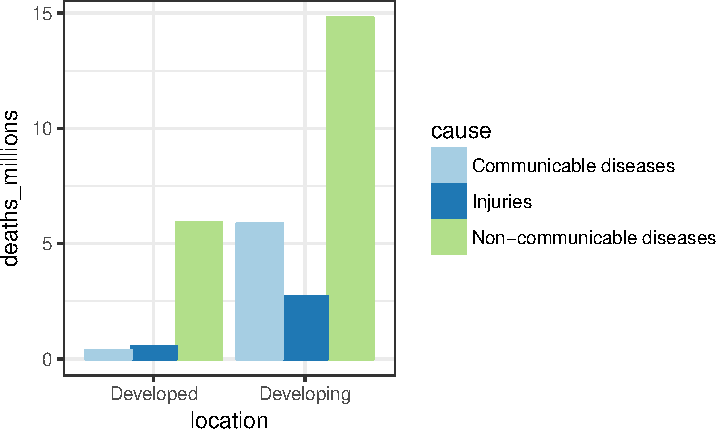
\includegraphics{01_first_interaction_files/figure-latex/unnamed-chunk-5-1.pdf}

\section{Facets (panels)}\label{facets-panels}

Going back to the dataframe with all years (1990 -- 2015), add
\texttt{facet\_wrap(\textasciitilde{}year)} to plot all years at once:

\begin{Shaded}
\begin{Highlighting}[]
\NormalTok{mydata }\OperatorTok\StringTok{ }
\StringTok{  }\KeywordTok{ggplot}\NormalTok{(}\KeywordTok{aes}\NormalTok{(}\DataTypeTok{x      =}\NormalTok{ location,}
             \DataTypeTok{y      =}\NormalTok{ deaths_millions,}
             \DataTypeTok{fill   =}\NormalTok{ cause,}
             \DataTypeTok{colour =}\NormalTok{ cause)) }\OperatorTok{+}
\StringTok{  }\KeywordTok{geom_col}\NormalTok{() }\OperatorTok{+}
\StringTok{  }\KeywordTok{facet_wrap}\NormalTok{(}\OperatorTok{~}\NormalTok{year)}
\end{Highlighting}
\end{Shaded}

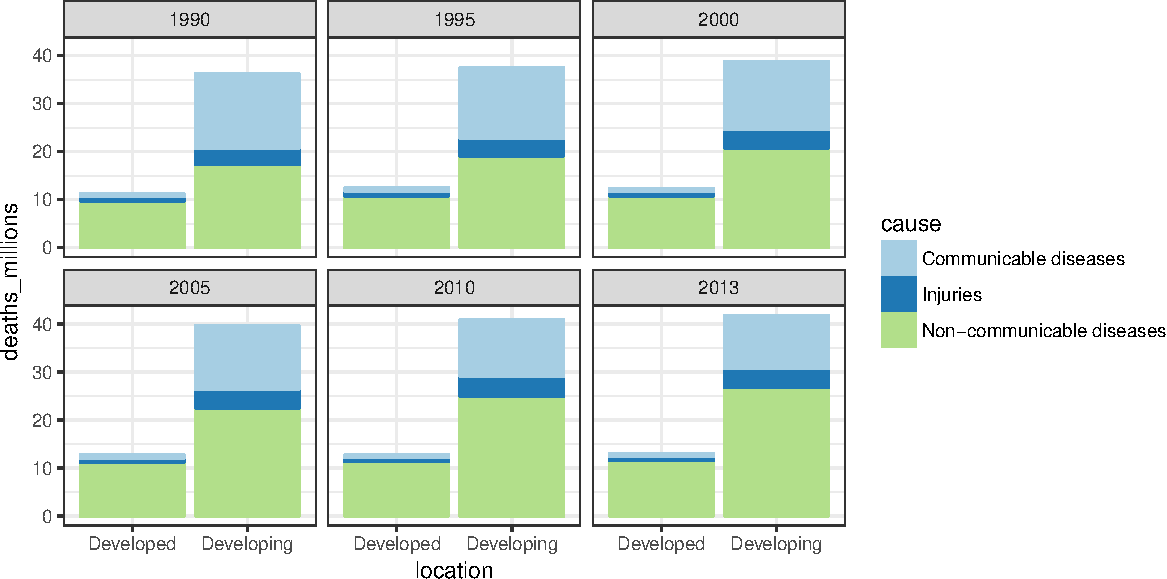
\includegraphics{01_first_interaction_files/figure-latex/unnamed-chunk-6-1.pdf}

\section{Extra: using aethetics outside of the
aes()}\label{extra-using-aethetics-outside-of-the-aes}

\subsection{Setting a constant fill}\label{setting-a-constant-fill}

Using the \texttt{mydata2013} example again, what does the addition of
\texttt{fill\ =\ "black"} in this code do? Note that putting the
\texttt{ggplot(aes())} code all on one line not affect the result.

\begin{Shaded}
\begin{Highlighting}[]
\NormalTok{mydata2013 }\OperatorTok\StringTok{ }
\StringTok{  }\KeywordTok{ggplot}\NormalTok{(}\KeywordTok{aes}\NormalTok{(}\DataTypeTok{x =}\NormalTok{ location, }\DataTypeTok{y =}\NormalTok{ deaths_millions, }\DataTypeTok{fill =}\NormalTok{ cause, }\DataTypeTok{colour =}\NormalTok{ cause)) }\OperatorTok{+}
\StringTok{  }\KeywordTok{geom_col}\NormalTok{(}\DataTypeTok{fill =} \StringTok{"black"}\NormalTok{)}
\end{Highlighting}
\end{Shaded}

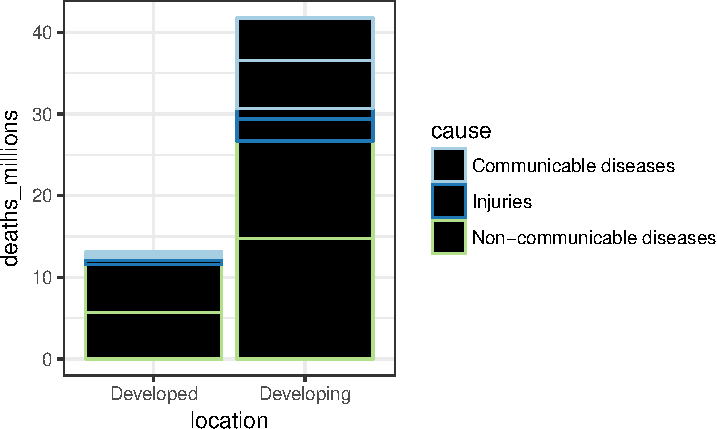
\includegraphics{01_first_interaction_files/figure-latex/unnamed-chunk-7-1.pdf}

Setting aesthetics (x, y, fill, colour, etc.) outside of \texttt{aes()}
sets them to a constant value. R can recognise of a lot of colour names,
e.g., try ``cornflowerblue'', ``firebrick'', or just ``red'', ``green'',
``blue'', etc. For a full list, Google ``Colours in R''. R also knows
HEX codes, e.g. \texttt{fill\ =\ "\#fec3fc"} is pink.

\subsection{Exercise}\label{exercise-1}

What is the difference between colour and fill in the context of a
barplot?

Hint: Use \texttt{colour\ =\ "black"} instead of
\texttt{fill\ =\ "black"} to investigate what \texttt{ggplot()} thinks a
colour is.

\begin{Shaded}
\begin{Highlighting}[]
\NormalTok{mydata2013 }\OperatorTok\StringTok{ }
\StringTok{  }\KeywordTok{ggplot}\NormalTok{(}\KeywordTok{aes}\NormalTok{(}\DataTypeTok{x =}\NormalTok{ location, }\DataTypeTok{y =}\NormalTok{ deaths_millions, }\DataTypeTok{fill =}\NormalTok{ cause, }\DataTypeTok{colour =}\NormalTok{ cause))}\OperatorTok{+}
\StringTok{  }\KeywordTok{geom_col}\NormalTok{(}\DataTypeTok{colour =} \StringTok{"black"}\NormalTok{)}
\end{Highlighting}
\end{Shaded}

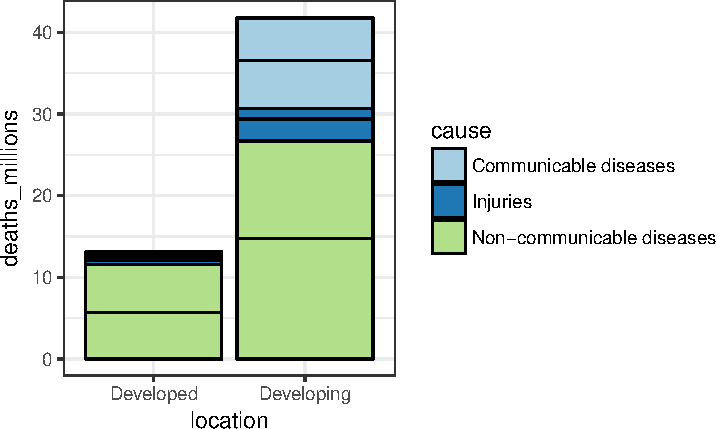
\includegraphics{01_first_interaction_files/figure-latex/unnamed-chunk-8-1.pdf}

\subsection{Exercise}\label{exercise-2}

Why are some of the words in our code quoted (e.g.
\texttt{fill\ =\ "black"}) whereas others are not (e.g.
\texttt{x\ =\ location})?

\section{\texorpdfstring{Two geoms for barplots: \texttt{geom\_bar()} or
\texttt{geom\_col()}}{Two geoms for barplots: geom\_bar() or geom\_col()}}\label{two-geoms-for-barplots-geom_bar-or-geom_col}

Both \texttt{geom\_bar()} and \texttt{geom\_col()} create barplots. If
you:

\begin{itemize}
\tightlist
\item
  Want to visualise the count of different lines in a dataset - use
  geom\_bar()

  \begin{itemize}
  \tightlist
  \item
    For example, if you are using a patient-level dataset (each line is
    a patient record):
    \texttt{mydata\ \%\textgreater{}\%\ \ \ ggplot(aes(x\ =\ sex))\ +\ \ geom\_bar()}
  \end{itemize}
\item
  Your dataset is already summarised - use geom\_col()

  \begin{itemize}
  \tightlist
  \item
    For example, in the GBD dataset we use here, each line already
    includes a summarised value (\texttt{deaths\_millions})
  \end{itemize}
\end{itemize}

If you have used R before, you might have come across
\texttt{geom\_bar(stat\ =\ "identity")} which is the same as
\texttt{geom\_col()}.

\section{Solutions}\label{solutions}

\textbf{1.2.1:} There is a double closing bracket because \texttt{aes()}
is wrapped inside \texttt{ggplot()} - \texttt{ggplot(aes())}.

\textbf{1.2.2:}

\begin{Shaded}
\begin{Highlighting}[]
\NormalTok{mydata2013 }\OperatorTok\StringTok{ }
\StringTok{  }\KeywordTok{ggplot}\NormalTok{(}\KeywordTok{aes}\NormalTok{(}\DataTypeTok{x      =}\NormalTok{ location,}
             \DataTypeTok{y      =}\NormalTok{ deaths_millions,}
             \DataTypeTok{fill   =}\NormalTok{ cause,}
             \DataTypeTok{colour =}\NormalTok{ cause)) }\OperatorTok{+}
\StringTok{  }\KeywordTok{geom_col}\NormalTok{()}
\end{Highlighting}
\end{Shaded}

\textbf{1.5.2:}

On a barplot, the colour aesthetic outlines the fill. In a later session
we will see, however, that for points and lines, colour is the main
aesthetic to define.

\textbf{1.5.3:}

Words in quotes are generally something are setting to a constant value
(e.g.~make all outlines black, rather than colour them based on the
cause they are representing). Unquoted words are generally variables (or
functions). If the word ``function'' just threw you, Google ``Jesse
Maegan: What the h*ck is a function"

\chapter{R Basics}\label{r-basics}

The aim of this module is to familiarise you with how R works and how to
read in and apply basic manipulations on your data. Here, we will be
working with similar but slightly shorter version of the Global Burden
of Disease dataset than we did for the bar plots.

Throughout this course, don't copy or type code directly into the
Console. We will only be using the Console for viewing output, warnings,
and errors. All code should be in a script and executed (=run) using
Control+Enter (line or section) or Control+Shift+Enter (whole script).
Make sure you are always working in a project (the right-top corner of
your RStudio interface should say ``HealthyR'').

\section{Getting help}\label{getting-help}

RStudio has a built in Help tab. To use the Help tab, move your cursor
to something in your code (e.g. \texttt{read\_csv()}) and press F1 -
this will show you the definition and some examples. However, the Help
tab is only useful if you already know what you are looking for but
can't remember how it worked exactly. For finding help on things you
have not used before, it is best to Google it. R has about 2 million
users so someone somewhere has had the same question or problem.

\section{Starting with a blank
canvas}\label{starting-with-a-blank-canvas}

In the first session we loaded some data that we then plotted. When we
import data, R remembers the data and stores it in the Environment tab.

It's good practice to clear the environment before starting new work, as
it's best to use fresh up to date data - otherwise we could accidentally
use data which has nothing to do with our work.

Try clearing and loading in the data again.

To clear data we can simply run the following code:

\begin{Shaded}
\begin{Highlighting}[]
\KeywordTok{rm}\NormalTok{(}\DataTypeTok{list=}\KeywordTok{ls}\NormalTok{())}
\end{Highlighting}
\end{Shaded}

We can also manually clear the environment in RStudio by clicking the
brush symbol underneath the Environment tab.

Sometimes just clearing the Environment tab is not enough - especially
if you are working with lots of different packages or other people's
scripts. You should also:

\begin{itemize}
\tightlist
\item
  Go to Tools -\textgreater{} Global Options -\textgreater{} General and
  set ``Save .RData on exit'' to Never. This does not mean you can't or
  shouldn't save your work in .RData files. But it is best to do it
  consciously and load exactly what you need to load, rather than
  letting R always save and load everything for you, as this could also
  include broken data or objects.
\item
  Restart R (Control+Shift+F10 or select it from Session -\textgreater{}
  Restart R).
\end{itemize}

\section{Working with Objects}\label{working-with-objects}

It's sometimes difficult to appreciate how coding works without trying
it first.

These exercises will show you how R works.

We'll first create an object and call it \texttt{a}, we will give the
object \texttt{a} a value of 1.

In R the equals \texttt{=} sign tells R to give the object on the left
of the sign the value of whatever is on the right of the sign.

\begin{Shaded}
\begin{Highlighting}[]
\NormalTok{a =}\StringTok{ }\DecValTok{1}
\end{Highlighting}
\end{Shaded}

In your environment panel, you should see \texttt{a} appear under the
\texttt{Values} section.

Now, lets create \texttt{b} and give it a value of 2.

\begin{Shaded}
\begin{Highlighting}[]
\NormalTok{b =}\StringTok{ }\DecValTok{2}
\end{Highlighting}
\end{Shaded}

Lets now add \texttt{a} and \texttt{b} together to create the object
\texttt{c}

\begin{Shaded}
\begin{Highlighting}[]
\NormalTok{c =}\StringTok{ }\NormalTok{a }\OperatorTok{+}\StringTok{ }\NormalTok{b }

\CommentTok{#Print the value of c to the Console}

\NormalTok{c }\CommentTok{# should return the number 3}
\end{Highlighting}
\end{Shaded}

\begin{verbatim}
## [1] 3
\end{verbatim}

All of R is just an extension of this: applying more complex functions
(calculations) across more complex objects.

It's important to appreciate that objects can be more than just single
numbers too. They can be entire spreadsheets, which in R are known as
\texttt{data\ frames}.

Note that many people use \texttt{\textless{}-} instead of \texttt{=}.
They mean the same thing in R. \texttt{=} and \texttt{\textless{}-} save
what is on the right into the name on the left. There is also a
left-to-right operator: \texttt{-\textgreater{}}.

\subsection{Exercise}\label{exercise-3}

Create 3 new variables, \texttt{d}, \texttt{e}, \texttt{f} with values
6, 7, 8 using the different assignment operators.

\begin{Shaded}
\begin{Highlighting}[]
\NormalTok{d  =}\StringTok{ }\DecValTok{6}
\NormalTok{e <-}\StringTok{ }\DecValTok{7}
\DecValTok{8}\NormalTok{ ->}\StringTok{ }\NormalTok{f}
\end{Highlighting}
\end{Shaded}

\section{Loading data}\label{loading-data}

Lets clear the environment again

\begin{Shaded}
\begin{Highlighting}[]
\KeywordTok{rm}\NormalTok{(}\DataTypeTok{list=}\KeywordTok{ls}\NormalTok{())}
\end{Highlighting}
\end{Shaded}

Now the environment is clear, lets load in the data:

\begin{Shaded}
\begin{Highlighting}[]
\KeywordTok{library}\NormalTok{(tidyverse)}\CommentTok{#Tidyverse is the package which contains some of the code we want to use}

\NormalTok{mydata =}\StringTok{ }\KeywordTok{read_csv}\NormalTok{(}\StringTok{"global_burden_disease_short.csv"}\NormalTok{)}
\end{Highlighting}
\end{Shaded}

But how can we look at the data we just loaded? How do we know which
variables it contains? Hint: the Environment tab.

\subsection{Excercise}\label{excercise}

Answer these question about your data:

\begin{enumerate}
\def\labelenumi{\arabic{enumi}.}
\item
  At present, how many variables are there?
\item
  How many deaths were there from communicable diseases in 1990? Hint:
  clicking on columns when Viewing a dataset orders it.
\end{enumerate}

\subsection{Other ways to investigate
objects}\label{other-ways-to-investigate-objects}

In most cases, you can rely on the Environment tab to see how many
variables you have. If, however, the dataset you are using is too big to
easily navigate within, you might need to use \texttt{names(mydata)},
\texttt{head(mydata)}, or \texttt{str(mydata)}.

Furthermore, we can select a single column using the dollar sign:
\texttt{\$}.

So if we type:

\begin{Shaded}
\begin{Highlighting}[]
\NormalTok{mydata}\OperatorTok{$}\NormalTok{deaths}
\end{Highlighting}
\end{Shaded}

\begin{verbatim}
##  [1] 16149409 26993493  4325788 15449045 29897069  4639869 14775502
##  [8] 31521934  4776852 13890709 33637815  4833919 12431802 36259550
## [15]  4970846 11809640 38267197  4786929
\end{verbatim}

R will give us all the data for that variable.

\subsection{Exercise}\label{exercise-4}

\begin{figure}
\centering

\includegraphics{images/magittr.png}
\caption{}
\end{figure}

*Image source:
\url{https://cran.r-project.org/web/packages/magrittr/vignettes/magrittr.html*}

Re-write \texttt{names(mydata)} and \texttt{head(mydata)} using the pipe
(\texttt{\%\textgreater{}\%}). Use the keyboard shortcut
\texttt{Control+Shift+M} to insert it.

\subsection{Exercise}\label{exercise-5}

How many unique values does the \texttt{cause} variable have? Hint:
\texttt{mydata\$cause} piped into \texttt{unique()} piped into
\texttt{length()}.

\section{Operators}\label{operators}

Operators are symbols in R Code that tell R how to handle different
pieces of data or objects.

Here are the main operators:

\texttt{=,\ \textless{}-,\ ==,\ \textless{},\ \textgreater{},\ \textless{}=,\ \textgreater{}=}

Some of these perform a test on data. A good example of this is the `=='
operator.

This tells R to compare two things and ask if they are equal. If they
are equal R will return `TRUE', if not R will return `FALSE'.

On your R cheat sheet, you can see what the others do. Here is a
reminder:

\begin{longtable}[]{@{}llll@{}}
\toprule
Symbol & What does & Example & Example result\tabularnewline
\midrule
\endhead
\texttt{=} or \texttt{\textless{}-} & assigns & \texttt{x\ =\ 2} & the
value of x is now 2\tabularnewline
\texttt{==} & Equal? & \texttt{x\ ==\ 2} & TRUE\tabularnewline
\texttt{!=} & Not equal? & \texttt{x\ !=\ 1} & TRUE\tabularnewline
\texttt{\textless{}} & Less than & \texttt{x\ \textless{}\ 2} &
FALSE\tabularnewline
\texttt{\textgreater{}} & Greater than & \texttt{x\ \textgreater{}\ 1} &
TRUE\tabularnewline
\texttt{\textless{}=} & Less than or equal to &
\texttt{x\ \textless{}=\ 2} & TRUE\tabularnewline
\texttt{\textgreater{}=} & Greater than or equal to &
\texttt{x\ \textgreater{}=\ 1} & TRUE\tabularnewline
\texttt{\%\textgreater{}\%} & sends data into a function &
\texttt{x\ \%\textgreater{}\%\ print()} & 2\tabularnewline
\texttt{::} & indicates package & \texttt{dplyr::count()} &
\texttt{count()} fn. from the \texttt{dplyr} package\tabularnewline
\texttt{-\textgreater{}} & assigns & \texttt{2\ -\textgreater{}\ x} &
the value of x is now 2\tabularnewline
\texttt{\&} & AND & \texttt{x\ \textgreater{}\ 1\ \&\ x\ \textless{}\ 3}
& TRUE\tabularnewline
\texttt{\textbar{}} & OR &
\texttt{x\ \textgreater{}\ 3\ \textbar{}\ x\ ==\ 3} &
TRUE\tabularnewline
\texttt{\%in\%} & is value in list & \texttt{x\ \%in\%\ c(1,2,3)} &
TRUE\tabularnewline
\texttt{\$} & select a column & \texttt{mydata\$year} &
1990,1996,\ldots{}\tabularnewline
\texttt{c()} & combines values & \texttt{c(1,\ 2)} & 1, 2\tabularnewline
\texttt{\#} & comment & \texttt{\#Riinu\ changed\ this} & ignored by
R\tabularnewline
\bottomrule
\end{longtable}

For example, if we wanted to select the years in the Global Burden of
disease study after 2000 (and including 2000) we could type the
following:

\begin{Shaded}
\begin{Highlighting}[]
\NormalTok{mydata }\OperatorTok\StringTok{ }
\StringTok{  }\KeywordTok{filter}\NormalTok{(year }\OperatorTok{>=}\StringTok{ }\DecValTok{2000}\NormalTok{)}
\end{Highlighting}
\end{Shaded}

To save this as a new object we would then write:

\begin{Shaded}
\begin{Highlighting}[]
\NormalTok{mydata_out =}\StringTok{ }\NormalTok{mydata }\OperatorTok\StringTok{ }
\StringTok{  }\KeywordTok{filter}\NormalTok{(year }\OperatorTok{>=}\StringTok{ }\DecValTok{2000}\NormalTok{)}

\CommentTok{#Or we could write}

\NormalTok{mydata }\OperatorTok\StringTok{ }
\StringTok{  }\KeywordTok{filter}\NormalTok{(year }\OperatorTok{>=}\StringTok{ }\DecValTok{2000}\NormalTok{) ->}\StringTok{ }\NormalTok{mydata_out}
\end{Highlighting}
\end{Shaded}

How would you change the above code to only include years greater than
2000 (so not including 2000 itself too)? Hint: look at the table of
operators above (also in your HealthyR QuickStart Sheet).

\subsection{Exercise}\label{exercise-6}

Modify the above example to filter for only year 2000, not all years
greater than 2000. Save it into a variable called
\texttt{mydata\_year2000}.

\subsection{Exercise}\label{exercise-7}

Let's practice this and combine multiple selections together.

This `\textbar{}' means OR and `\&' means AND.

From \texttt{mydata}, select the lines where year is either 1990 or 2013
and cause is ``Communicable diseases'':

\begin{Shaded}
\begin{Highlighting}[]
\NormalTok{new_data_selection =}\StringTok{ }\NormalTok{mydata }\OperatorTok\StringTok{ }
\StringTok{  }\KeywordTok{filter}\NormalTok{( (year }\OperatorTok{==}\StringTok{ }\DecValTok{1990} \OperatorTok{|}\StringTok{ }\NormalTok{year }\OperatorTok{==}\StringTok{ }\DecValTok{2013}\NormalTok{) }\OperatorTok{&}\StringTok{ }\NormalTok{cause }\OperatorTok{==}\StringTok{ "Communicable diseases"}\NormalTok{)}

\CommentTok{# or we can get rid of the extra brackets around the years}
\CommentTok{# by moving cause into a new filter on a new line:}

\NormalTok{new_data_selection =}\StringTok{ }\NormalTok{mydata }\OperatorTok\StringTok{ }
\StringTok{  }\KeywordTok{filter}\NormalTok{( year }\OperatorTok{==}\StringTok{ }\DecValTok{1990} \OperatorTok{|}\StringTok{ }\NormalTok{year }\OperatorTok{==}\StringTok{ }\DecValTok{2013}\NormalTok{) }\OperatorTok\StringTok{ }
\StringTok{  }\KeywordTok{filter}\NormalTok{( cause }\OperatorTok{==}\StringTok{ "Communicable diseases"}\NormalTok{ )}
\end{Highlighting}
\end{Shaded}

\section{Types of variables}\label{types-of-variables}

Like many other types of statistical software, R needs to know what is
the variable type of each column. The main types are:

\subsection{Characters}\label{characters}

\textbf{Characters} (sometimes referred to as \emph{strings} or
\emph{character strings}) in R are letters, words, or even whole
sentences (an example of this may be free text comments). We can specify
these using the \texttt{as.character()} function. Characters are
displayed in-between \texttt{""} (or
\texttt{\textquotesingle{}\textquotesingle{}}).

\subsection{Factors}\label{factors}

\textbf{Factors} are fussy characters. Factors are fussy because they
have something called levels. Levels are all the unique values this
variable could take - e.g.~like when we looked at
\texttt{mydata\$cause\ \%\textgreater{}\%\ unique()}. Using factors
rather than just characters can be useful because:

\begin{itemize}
\tightlist
\item
  The values factor levels can take is fixed. For example, if the levels
  of your column called \texttt{sex} are ``Male'' and ``Female'' and you
  try to add a new patient where sex is called just ``F'' you will get a
  warning from R. If \texttt{sex} was a character column rather than a
  factor R would have no problem with this and you would end up with
  ``Male'', ``Female'', and ``F'' in your your column.
\item
  Levels have an order. When we plotted the different causes of death in
  the last session, R ordered them alphabetically (because
  \texttt{cause} was a character rather than a factor). But if you want
  to use a non-alphabetical order, e.g. ``Communicable
  diseases''-``Non-communicable diseases''-``Injuries'', we need make
  \texttt{cause} into a factor. Making a character column into a factor
  enables us to define and change the order of the levels. Furthermore,
  there are useful tools such as \texttt{fct\_inorder} or
  \texttt{fct\_infreq} that can order factor levels for us.
\end{itemize}

These can be huge benefits, especially as a lot of medical data analyses
include comparing different risks to a reference level. Nevertheless,
the fussiness of factors can sometimes be unhelpful or even frustrating.
For example, if you really did want to add a new level to your
\texttt{gender} column (e.g., ``Prefer not to say'') you will either
have to convert the column to a character, add it, and convert it back
to a factor, or use \texttt{fct\_expand} to add the level and then add
your new line.

\subsubsection{Exercise}\label{exercise-8}

Temporarily type \texttt{fct\_inorder} anywhere in your script, then
press F1. Read the \textbf{Description} in the Help tab and discuss with
your neighbour how \texttt{fct\_inorder} and \texttt{fct\_infreq} would
order your factor levels.

\subsection{Numbers}\label{numbers}

Self-explanatory! These are numbers. In R, we specify these using the
\texttt{as.numeric()} function. Numbers without decimal places are
sometimes called integers. Click on the blue arrow in front of
\texttt{mydata} in the Environment tab and see that \texttt{year} is an
\texttt{int} whereas \texttt{deaths} is a \texttt{num}.

\subsection{Specifying variable types}\label{specifying-variable-types}

\begin{Shaded}
\begin{Highlighting}[]
\KeywordTok{as.character}\NormalTok{(mydata}\OperatorTok{$}\NormalTok{cause)}

\KeywordTok{as.numeric}\NormalTok{(mydata}\OperatorTok{$}\NormalTok{year)}

\KeywordTok{factor}\NormalTok{(mydata}\OperatorTok{$}\NormalTok{year)}

\CommentTok{#Lets save the cause as a factor}

\NormalTok{mydata}\OperatorTok{$}\NormalTok{cause =}\StringTok{ }\KeywordTok{factor}\NormalTok{(mydata}\OperatorTok{$}\NormalTok{cause)}

\CommentTok{#Now lets print it out}

\NormalTok{mydata}\OperatorTok{$}\NormalTok{cause}
\end{Highlighting}
\end{Shaded}

\subsection{Exercise}\label{exercise-9}

Change the order of the levels in \texttt{mydata\$cause} so that
``Non-communicable diseases'' come before ``Injuries''. Hint: use F1 to
investigate examples of how \texttt{fct\_relevel()} works.

\section{Importing data}\label{importing-data}

For historical reasons, R's default functions (e.g. \texttt{read.csv()}
or \texttt{data.frame()}) convert all characters to factors
automatically (for more on this see
\href{http://forcats.tidyverse.org}{forcats.tidyverse.org}. But it is
usually more convenient to deal with characters and convert some of the
columns to factors when necessary.

Base R:

\begin{Shaded}
\begin{Highlighting}[]
\NormalTok{mydata =}\StringTok{ }\KeywordTok{read.csv}\NormalTok{(}\StringTok{"global_burden_disease_short.csv"}\NormalTok{, }\DataTypeTok{stringsAsFactors =} \OtherTok{FALSE}\NormalTok{)}
\end{Highlighting}
\end{Shaded}

The tidyverse version, \texttt{read\_csv()}, has
\texttt{stringsAsFactors} set to FALSE by default (and it is a lot
faster than \texttt{read.csv()} when reading in large datasets).

Tidyverse:

\begin{Shaded}
\begin{Highlighting}[]
\NormalTok{mydata =}\StringTok{ }\KeywordTok{read_csv}\NormalTok{(}\StringTok{"global_burden_disease_short.csv"}\NormalTok{)}
\end{Highlighting}
\end{Shaded}

\begin{verbatim}
## Parsed with column specification:
## cols(
##   cause = col_character(),
##   year = col_integer(),
##   deaths = col_double()
## )
\end{verbatim}

You can use the ``Import Dataset'' button in the Environment tab to get
the code for importing data from Excel, SPSS, SAS, or Stata.

\section{Adding columns to
dataframes}\label{adding-columns-to-dataframes}

If we wanted to add in a new column or variable to our data, we can
simply can use the dollar sign `\$' to create a new variable inside a
pre-existing piece of data:

\begin{Shaded}
\begin{Highlighting}[]
\NormalTok{mydata}\OperatorTok{$}\NormalTok{new =}\StringTok{ }\DecValTok{1}

\NormalTok{mydata}\OperatorTok{$}\NormalTok{new2 =}\StringTok{ }\DecValTok{1}\OperatorTok{:}\DecValTok{18}
\end{Highlighting}
\end{Shaded}

Run these lines and click on \texttt{mydata} in the Environment tab to
check this worked as expected.

Conversely, if we want to delete a specific variable or column we can
use the `NULL' function, or alternatively ask R to \texttt{select()} the
data without the new variable included.

\begin{Shaded}
\begin{Highlighting}[]
\NormalTok{mydata}\OperatorTok{$}\NormalTok{new =}\StringTok{ }\OtherTok{NULL}

\NormalTok{mydata =}\StringTok{ }\NormalTok{mydata }\OperatorTok\StringTok{ }
\StringTok{  }\KeywordTok{select}\NormalTok{(}\OperatorTok{-}\NormalTok{new2)}
\end{Highlighting}
\end{Shaded}

We can make new variables using calculations based on variables in the
data too.

The mutate function is useful here. All you have to specify within the
mutate function is the name of the variable (this can be new or
pre-existing) and where the new data should come from.

There are two equivalent ways of defining new columns based on a
calculation with a previous column:

\begin{Shaded}
\begin{Highlighting}[]
\CommentTok{#First option}

\NormalTok{mydata}\OperatorTok{$}\NormalTok{years_from_}\DecValTok{1990}\NormalTok{ =}\StringTok{ }\NormalTok{mydata}\OperatorTok{$}\NormalTok{year }\OperatorTok{-}\StringTok{ }\DecValTok{1990} 
\NormalTok{mydata}\OperatorTok{$}\NormalTok{deaths_millions =}\StringTok{ }\NormalTok{mydata}\OperatorTok{$}\NormalTok{deaths}\OperatorTok{/}\DecValTok{1000000}

\CommentTok{#Second option (mutate() function)}

\NormalTok{mydata =}\StringTok{ }\NormalTok{mydata }\OperatorTok\StringTok{ }
\StringTok{  }\KeywordTok{mutate}\NormalTok{(}\DataTypeTok{years_from_1990 =}\NormalTok{ year}\OperatorTok{-}\DecValTok{1990}\NormalTok{,}
         \DataTypeTok{deaths_millions =}\NormalTok{ deaths}\OperatorTok{/}\DecValTok{1000000}\NormalTok{) }
\end{Highlighting}
\end{Shaded}

Throughout this course we will be using both of these ways to create or
modify columns. The first option (using the \texttt{\$}) can look neater
when changing a single variable, but when combining multiple ones you
will end up repeating \texttt{mydata\$}. \texttt{mutate()} removes the
duplication, but it does add a new line and brackets.

\section{Rounding numbers}\label{rounding-numbers}

We can use \texttt{round()} to round the new variables to create
integers.

\subsection{Exercise}\label{exercise-10}

Round the new column \texttt{deaths\_millions} to no decimals:

\begin{verbatim}
##  [1] 16 27  4 15 30  5 15 32  5 14 34  5 12 36  5 12 38  5
\end{verbatim}

How would you round it to 2 decimals? Hint: use F1 to investigate
\texttt{round()}. What do \texttt{ceiling()} and \texttt{floor()} do?

\section{The combine function: c()}\label{the-combine-function-c}

The combine function combines several values: \texttt{c()}

The combine function can be used with numbers or characters (like words
or letters):

\begin{Shaded}
\begin{Highlighting}[]
\NormalTok{examplelist =}\StringTok{ }\KeywordTok{c}\NormalTok{(}\StringTok{"Red"}\NormalTok{, }\StringTok{"Yellow"}\NormalTok{, }\StringTok{"Green"}\NormalTok{, }\StringTok{"Blue"}\NormalTok{)}

\CommentTok{# Ask R to print it by executing it on its own line}

\NormalTok{examplelist}
\end{Highlighting}
\end{Shaded}

\begin{verbatim}
## [1] "Red"    "Yellow" "Green"  "Blue"
\end{verbatim}

\subsection{Exercise}\label{exercise-11}

There are 18 lines (observations) in mydata. Create a new variable using
\texttt{c()} with 18 values (numbers, words, whichever you like,
e.g.~like we created \texttt{examplelist}). Then add it as new column to
\texttt{mydata\$newlist}. Advanced version: do this using a combination
of \texttt{rep()} and \texttt{c()}.

\newpage

\section{\texorpdfstring{The \texttt{paste()}
function}{The paste() function}}\label{the-paste-function}

The \texttt{paste()} function is used to paste several words or numbers
into one character variable/sentence.

In the paste function we need to specify what we would like to combine,
and what should separate the components. By default, the separation is a
space, but we can change this using the \texttt{sep\ =} option within
the paste function.

So, for example if we wanted to make a sentence:

\begin{Shaded}
\begin{Highlighting}[]
\KeywordTok{paste}\NormalTok{(}\StringTok{"Edinburgh"}\NormalTok{, }\StringTok{"is"}\NormalTok{, }\StringTok{"Great"}\NormalTok{)}
\end{Highlighting}
\end{Shaded}

\begin{verbatim}
## [1] "Edinburgh is Great"
\end{verbatim}

\begin{Shaded}
\begin{Highlighting}[]
\CommentTok{#Lets add in full stops}

\KeywordTok{paste}\NormalTok{(}\StringTok{"Edinburgh"}\NormalTok{, }\StringTok{"is"}\NormalTok{, }\StringTok{"Great"}\NormalTok{, }\DataTypeTok{sep =} \StringTok{"."}\NormalTok{)}
\end{Highlighting}
\end{Shaded}

\begin{verbatim}
## [1] "Edinburgh.is.Great"
\end{verbatim}

\begin{Shaded}
\begin{Highlighting}[]
\CommentTok{#separator needs to go in "" as it is a character}

\CommentTok{#If we really like Edinburgh}

\KeywordTok{paste}\NormalTok{(}\StringTok{"Edinburgh"}\NormalTok{, }\StringTok{"is"}\NormalTok{, }\StringTok{"Great"}\NormalTok{, }\DataTypeTok{sep =} \StringTok{"!"}\NormalTok{)}
\end{Highlighting}
\end{Shaded}

\begin{verbatim}
## [1] "Edinburgh!is!Great"
\end{verbatim}

\begin{Shaded}
\begin{Highlighting}[]
\CommentTok{#If we want to make it one word}

\KeywordTok{paste}\NormalTok{(}\StringTok{"Edinburgh"}\NormalTok{, }\StringTok{"is"}\NormalTok{, }\StringTok{"Great"}\NormalTok{, }\DataTypeTok{sep =} \StringTok{""}\NormalTok{) }\CommentTok{# no separator (still need the brackets)}
\end{Highlighting}
\end{Shaded}

\begin{verbatim}
## [1] "EdinburghisGreat"
\end{verbatim}

We can also join two different variables together using
\texttt{paste()}:

\begin{Shaded}
\begin{Highlighting}[]
\KeywordTok{paste}\NormalTok{(}\StringTok{"Year is"}\NormalTok{, mydata}\OperatorTok{$}\NormalTok{year)}
\end{Highlighting}
\end{Shaded}

\begin{verbatim}
##  [1] "Year is 1990" "Year is 1990" "Year is 1990" "Year is 1995"
##  [5] "Year is 1995" "Year is 1995" "Year is 2000" "Year is 2000"
##  [9] "Year is 2000" "Year is 2005" "Year is 2005" "Year is 2005"
## [13] "Year is 2010" "Year is 2010" "Year is 2010" "Year is 2013"
## [17] "Year is 2013" "Year is 2013"
\end{verbatim}

\subsection{Exercise}\label{exercise-12}

Fix this code:

Hint: Think about characters and quotes!

\begin{Shaded}
\begin{Highlighting}[]
\KeywordTok{paste}\NormalTok{(Today is, }\KeywordTok{Sys.Date}\NormalTok{() )}
\end{Highlighting}
\end{Shaded}

\section{Combining two dataframes}\label{combining-two-dataframes}

For combining dataframes based on shared variables we use the Joins:
\texttt{left\_join()}, \texttt{right\_join()}, \texttt{inner\_join()},
or \texttt{full\_join()}. Let's split some of the variables in
\texttt{mydata} between two new dataframes: \texttt{first\_data} and
\texttt{second\_data}. For demonstrating the difference between the
different joins, we will only include a subset (first 6 rows) of the
dataset in \texttt{second\_data}:

\begin{Shaded}
\begin{Highlighting}[]
\NormalTok{first_data  =}\StringTok{ }\KeywordTok{select}\NormalTok{(mydata, year, cause, deaths_millions)}
\NormalTok{second_data =}\StringTok{ }\KeywordTok{select}\NormalTok{(mydata, year, cause, deaths) }\OperatorTok\StringTok{ }\KeywordTok{slice}\NormalTok{(}\DecValTok{1}\OperatorTok{:}\DecValTok{6}\NormalTok{)}

\CommentTok{#change the order of rows in first_data to demosntrate the join does not rely on the ordering of rows:}
\NormalTok{first_data =}\StringTok{ }\KeywordTok{arrange}\NormalTok{(first_data, deaths_millions)}

\NormalTok{combined_left  =}\StringTok{  }\KeywordTok{left_join}\NormalTok{(first_data, second_data)}
\NormalTok{combined_right =}\StringTok{ }\KeywordTok{right_join}\NormalTok{(first_data, second_data)}
\NormalTok{combined_inner =}\StringTok{ }\KeywordTok{inner_join}\NormalTok{(first_data, second_data)}
\NormalTok{combined_full  =}\StringTok{  }\KeywordTok{full_join}\NormalTok{(first_data, second_data)}
\end{Highlighting}
\end{Shaded}

Those who have used R before, or those who come across older scripts
will have seen \texttt{merge()} instead of the joins. \texttt{merge()}
works similarly to joins, but instead of having the four options defined
clearly at the front, you would have had to use the
\texttt{all\ =\ FALSE,\ all.x\ =\ all,\ all.y\ =\ all} arguments.

\begin{figure}
\centering

\includegraphics{images/databasejoke.jpg}
\caption{}
\end{figure}

\subsection{Exercise}\label{exercise-13}

Investigate the four new dataframes (\texttt{combined\_}) using the
Environment tab and discuss how the different joins (left, right, inner,
full) work.

\section{\texorpdfstring{The \texttt{summary()}
Function}{The summary() Function}}\label{the-summary-function}

In R, the \texttt{summary()} function provides a quick way of
summarising both data or the results of statistical tests.

Lets get a quick summary of all the variables inside the Global Burden
of Disease dataset. It will work for whole datasets and single variables
too.

\begin{Shaded}
\begin{Highlighting}[]
\NormalTok{mydata }\OperatorTok\StringTok{ }\KeywordTok{summary}\NormalTok{()}
\end{Highlighting}
\end{Shaded}

\begin{verbatim}
##     cause                year          deaths         years_from_1990
##  Length:18          Min.   :1990   Min.   : 4325788   Min.   : 0.00  
##  Class :character   1st Qu.:1995   1st Qu.: 4868151   1st Qu.: 5.00  
##  Mode  :character   Median :2002   Median :14333106   Median :12.50  
##                     Mean   :2002   Mean   :17189854   Mean   :12.17  
##                     3rd Qu.:2010   3rd Qu.:29171175   3rd Qu.:20.00  
##                     Max.   :2013   Max.   :38267197   Max.   :23.00  
##  deaths_millions
##  Min.   : 4.00  
##  1st Qu.: 5.00  
##  Median :14.50  
##  Mean   :17.22  
##  3rd Qu.:29.25  
##  Max.   :38.00
\end{verbatim}

This even works on statistical tests (we will learn more about these
later):

\begin{Shaded}
\begin{Highlighting}[]
\CommentTok{# lm stands for linear model}
\KeywordTok{lm}\NormalTok{(deaths }\OperatorTok{~}\StringTok{ }\NormalTok{year, }\DataTypeTok{data =}\NormalTok{ mydata) }\OperatorTok\StringTok{ }\KeywordTok{summary}\NormalTok{()}
\end{Highlighting}
\end{Shaded}

\begin{verbatim}
## 
## Call:
## lm(formula = deaths ~ year, data = mydata)
## 
## Residuals:
##       Min        1Q    Median        3Q       Max 
## -13480641 -11791203  -2889909  12818624  19999627 
## 
## Coefficients:
##               Estimate Std. Error t value Pr(>|t|)
## (Intercept) -181988644  736014812  -0.247    0.808
## year             99482     367606   0.271    0.790
## 
## Residual standard error: 12590000 on 16 degrees of freedom
## Multiple R-squared:  0.004556,   Adjusted R-squared:  -0.05766 
## F-statistic: 0.07324 on 1 and 16 DF,  p-value: 0.7901
\end{verbatim}

\subsection{When pipe sends data to the wrong
place}\label{when-pipe-sends-data-to-the-wrong-place}

Note that our usual way of doing things with the pipe would not work
here:

\begin{Shaded}
\begin{Highlighting}[]
\NormalTok{mydata }\OperatorTok\StringTok{ }
\StringTok{  }\KeywordTok{lm}\NormalTok{(deaths }\OperatorTok{~}\StringTok{ }\NormalTok{year) }\OperatorTok
\StringTok{  }\KeywordTok{summary}\NormalTok{()}
\end{Highlighting}
\end{Shaded}

This is because the pipe tries to send data into the first place of the
function (first argument), but \texttt{lm()} wants the formula
(\texttt{deaths\ \textasciitilde{}\ year}) first, then the dataframe. We
can bypass this using \texttt{data\ =\ .} to tell the pipe where to send
mydata:

\begin{Shaded}
\begin{Highlighting}[]
\NormalTok{mydata }\OperatorTok\StringTok{ }
\StringTok{  }\KeywordTok{lm}\NormalTok{(deaths }\OperatorTok{~}\StringTok{ }\NormalTok{year, }\DataTypeTok{data =}\NormalTok{ .) }\OperatorTok
\StringTok{  }\KeywordTok{summary}\NormalTok{()}
\end{Highlighting}
\end{Shaded}

\subsection{Exercise}\label{exercise-14}

Try adding a new variable called \texttt{death\_over\_10m} which
indicates whether there were 10 million deaths or more for each cause.
The new variable should take the form `Yes' or `No'.

Then make it a factor.

Then use \texttt{summary()} to find out about it!

\begin{Shaded}
\begin{Highlighting}[]
\NormalTok{mydata =}\StringTok{ }\NormalTok{mydata }\OperatorTok\StringTok{ }
\StringTok{  }\KeywordTok{mutate}\NormalTok{(}\DataTypeTok{death_over_10m =} \KeywordTok{ifelse}\NormalTok{(deaths }\OperatorTok{>=}\StringTok{ }\DecValTok{10000000}\NormalTok{, }\StringTok{"Yes"}\NormalTok{, }\StringTok{"No"}\NormalTok{)) }\CommentTok{#Using ifelse}

\NormalTok{mydata}\OperatorTok{$}\NormalTok{death_over_10m =}\StringTok{ }\KeywordTok{as.factor}\NormalTok{(mydata}\OperatorTok{$}\NormalTok{death_over_10m)}

\NormalTok{mydata}\OperatorTok{$}\NormalTok{death_over_10m }\OperatorTok\StringTok{ }\KeywordTok{summary}\NormalTok{()}
\end{Highlighting}
\end{Shaded}

\begin{verbatim}
##  No Yes 
##   6  12
\end{verbatim}

\section{Extra: Creating a dataframe from
scratch}\label{extra-creating-a-dataframe-from-scratch}

It is rare that you will need to create a dataframe by hand as most of
the time you will be reading in a data from a .csv or similar. But in
some cases (e.g., when creating special labels for a plot) it might be
useful, so this is how to create one:

\begin{Shaded}
\begin{Highlighting}[]
\NormalTok{patient_id =}\StringTok{ }\KeywordTok{paste0}\NormalTok{(}\StringTok{"ID"}\NormalTok{, }\DecValTok{1}\OperatorTok{:}\DecValTok{10}\NormalTok{)}
\NormalTok{sex        =}\StringTok{ }\KeywordTok{rep}\NormalTok{(}\KeywordTok{c}\NormalTok{(}\StringTok{"Female"}\NormalTok{, }\StringTok{"Male"}\NormalTok{), }\DecValTok{5}\NormalTok{)}
\NormalTok{age        =}\StringTok{ }\DecValTok{18}\OperatorTok{:}\DecValTok{27}

\NormalTok{newdata =}\StringTok{ }\KeywordTok{data_frame}\NormalTok{(patient_id, sex, age)}

\CommentTok{#same as}

\NormalTok{newdata      =}\StringTok{ }\KeywordTok{data_frame}\NormalTok{(}
  \DataTypeTok{patient_id =} \KeywordTok{paste0}\NormalTok{(}\StringTok{"ID"}\NormalTok{, }\DecValTok{1}\OperatorTok{:}\DecValTok{10}\NormalTok{), }\CommentTok{#note the commas}
  \DataTypeTok{sex        =} \KeywordTok{rep}\NormalTok{(}\KeywordTok{c}\NormalTok{(}\StringTok{"Female"}\NormalTok{, }\StringTok{"Male"}\NormalTok{), }\DecValTok{5}\NormalTok{),}
  \DataTypeTok{age        =} \DecValTok{18}\OperatorTok{:}\DecValTok{27}
\NormalTok{)}
\end{Highlighting}
\end{Shaded}

If we used \texttt{data.frame()} instead of \texttt{data\_frame()}, all
our character variables (\texttt{patient\_id}, \texttt{sex}) would
become factors automatically. This might make sense for \texttt{sex},
but it doesn't for \texttt{patient\_id}.

\subsection{Exercise}\label{exercise-15}

Create a new dataframe called \texttt{my\_dataframe} that looks like
this:

Hint: Use the functions \texttt{paste0()}, \texttt{seq()} and
\texttt{rep()}

\begin{verbatim}
## # A tibble: 10 x 3
##    patient_id   age    sex
##         <chr> <dbl>  <chr>
##  1       ID11    15   Male
##  2       ID12    20   Male
##  3       ID13    25   Male
##  4       ID14    30   Male
##  5       ID15    35   Male
##  6       ID16    40 Female
##  7       ID17    45 Female
##  8       ID18    50 Female
##  9       ID19    55 Female
## 10       ID20    60 Female
\end{verbatim}

\section{Solutions}\label{solutions-1}

\textbf{2.5.3}

\begin{Shaded}
\begin{Highlighting}[]
\NormalTok{mydata }\OperatorTok\StringTok{ }\KeywordTok{names}\NormalTok{()}
\NormalTok{mydata }\OperatorTok\StringTok{ }\KeywordTok{head}\NormalTok{()}
\NormalTok{mydata }\OperatorTok\StringTok{ }\KeywordTok{str}\NormalTok{()}
\end{Highlighting}
\end{Shaded}

\textbf{2.5.4}

\begin{Shaded}
\begin{Highlighting}[]
\NormalTok{mydata}\OperatorTok{$}\NormalTok{cause }\OperatorTok\StringTok{ }\KeywordTok{unique}\NormalTok{() }\OperatorTok\StringTok{ }\KeywordTok{length}\NormalTok{()}
\end{Highlighting}
\end{Shaded}

\begin{verbatim}
## [1] 3
\end{verbatim}

\textbf{2.6.2}

\begin{Shaded}
\begin{Highlighting}[]
\NormalTok{mydata_year2000 =}\StringTok{ }\NormalTok{mydata }\OperatorTok\StringTok{ }
\StringTok{  }\KeywordTok{filter}\NormalTok{(year }\OperatorTok{==}\StringTok{ }\DecValTok{2000}\NormalTok{)}
\end{Highlighting}
\end{Shaded}

\textbf{2.7.5}

\begin{Shaded}
\begin{Highlighting}[]
\NormalTok{mydata}\OperatorTok{$}\NormalTok{cause }\OperatorTok\StringTok{ }\KeywordTok{fct_relevel}\NormalTok{(}\StringTok{"Injuries"}\NormalTok{, }\DataTypeTok{after =} \DecValTok{1}\NormalTok{)}
\end{Highlighting}
\end{Shaded}

\textbf{2.10.1}

\begin{Shaded}
\begin{Highlighting}[]
\NormalTok{mydata}\OperatorTok{$}\NormalTok{deaths_millions =}\StringTok{ }\KeywordTok{round}\NormalTok{(mydata}\OperatorTok{$}\NormalTok{deaths_millions)}

\CommentTok{# or}
\NormalTok{mydata}\OperatorTok{$}\NormalTok{deaths_millions =}\StringTok{ }\NormalTok{mydata}\OperatorTok{$}\NormalTok{deaths_millions }\OperatorTok\StringTok{ }\KeywordTok{round}\NormalTok{()}

\CommentTok{# or even (load magrittr to get the superpower pipe - %<>%)}

\KeywordTok{library}\NormalTok{(magrittr)}

\NormalTok{mydata}\OperatorTok{$}\NormalTok{deaths_millions }\OperatorTok\StringTok{ }\KeywordTok{round}\NormalTok{()}
\end{Highlighting}
\end{Shaded}

\textbf{2.11.1}

\begin{Shaded}
\begin{Highlighting}[]
\NormalTok{examplelist =}\StringTok{ }\KeywordTok{c}\NormalTok{(}\StringTok{"Red"}\NormalTok{, }\StringTok{"Yellow"}\NormalTok{, }\StringTok{"Green"}\NormalTok{, }\StringTok{"Blue"}\NormalTok{,}
                \StringTok{"Red"}\NormalTok{, }\StringTok{"Yellow"}\NormalTok{, }\StringTok{"Green"}\NormalTok{, }\StringTok{"Blue"}\NormalTok{,}
                \StringTok{"Red"}\NormalTok{, }\StringTok{"Yellow"}\NormalTok{, }\StringTok{"Green"}\NormalTok{, }\StringTok{"Blue"}\NormalTok{,}
                \StringTok{"Red"}\NormalTok{, }\StringTok{"Yellow"}\NormalTok{, }\StringTok{"Green"}\NormalTok{, }\StringTok{"Blue"}\NormalTok{,}
                \StringTok{"Green"}\NormalTok{, }\StringTok{"Blue"}\NormalTok{)}

\CommentTok{#Let's see what we've made by using print}

\NormalTok{mydata}\OperatorTok{$}\NormalTok{newlist =}\StringTok{ }\NormalTok{examplelist}


\CommentTok{# using rep()}

\NormalTok{examplelist2 =}\StringTok{ }\KeywordTok{rep}\NormalTok{(}\KeywordTok{c}\NormalTok{(}\StringTok{"Green"}\NormalTok{, }\StringTok{"Red"}\NormalTok{), }\DecValTok{9}\NormalTok{)}
\end{Highlighting}
\end{Shaded}

\textbf{2.12.1}

\begin{Shaded}
\begin{Highlighting}[]
\KeywordTok{paste}\NormalTok{(}\StringTok{"Today is"}\NormalTok{, }\KeywordTok{Sys.Date}\NormalTok{())}
\end{Highlighting}
\end{Shaded}

\textbf{2.15.1}

\begin{Shaded}
\begin{Highlighting}[]
\NormalTok{my_dataframe =}\StringTok{ }\KeywordTok{data_frame}\NormalTok{(}
  \DataTypeTok{patient_id =} \KeywordTok{paste0}\NormalTok{(}\StringTok{"ID"}\NormalTok{, }\DecValTok{11}\OperatorTok{:}\DecValTok{20}\NormalTok{),}
  \DataTypeTok{age        =} \KeywordTok{seq}\NormalTok{(}\DecValTok{15}\NormalTok{, }\DecValTok{60}\NormalTok{, }\DecValTok{5}\NormalTok{),}
  \DataTypeTok{sex        =} \KeywordTok{c}\NormalTok{( }\KeywordTok{rep}\NormalTok{(}\StringTok{"Male"}\NormalTok{, }\DecValTok{5}\NormalTok{), }\KeywordTok{rep}\NormalTok{(}\StringTok{"Female"}\NormalTok{, }\DecValTok{5}\NormalTok{))}
\NormalTok{)}
\end{Highlighting}
\end{Shaded}

\chapter{Summarising data}\label{summarising-data}

In this session we will get to know our three best friends for
summarising data: \texttt{group\_by()}, \texttt{summarise()}, and
\texttt{mutate()}.

\section{Data}\label{data-1}

In Session 2, we used a very condensed version of the Global Burden of
Disease data. In this module we are going back to a longer one and we
will learn how to summarise it ourselves.

\begin{Shaded}
\begin{Highlighting}[]
\KeywordTok{source}\NormalTok{(}\StringTok{"1_source_theme.R"}\NormalTok{)}
\KeywordTok{load}\NormalTok{(}\StringTok{"global_burden_disease_long.rda"}\NormalTok{)}
\end{Highlighting}
\end{Shaded}

We were already using this longer dataset in Session1, but with
\texttt{colour=cause} to hide the fact that the total deaths in each
year was made up of 12 lines groups of data (as the black lines on the
bars indicate):

\begin{Shaded}
\begin{Highlighting}[]
\NormalTok{mydata }\OperatorTok\StringTok{ }
\StringTok{    }\KeywordTok{ggplot}\NormalTok{(}\KeywordTok{aes}\NormalTok{(}\DataTypeTok{x=}\NormalTok{year, }\DataTypeTok{y=}\NormalTok{deaths_millions, }\DataTypeTok{fill=}\NormalTok{cause))}\OperatorTok{+}\StringTok{ }
\StringTok{    }\KeywordTok{geom_col}\NormalTok{(}\DataTypeTok{colour =} \StringTok{"black"}\NormalTok{)}
\end{Highlighting}
\end{Shaded}

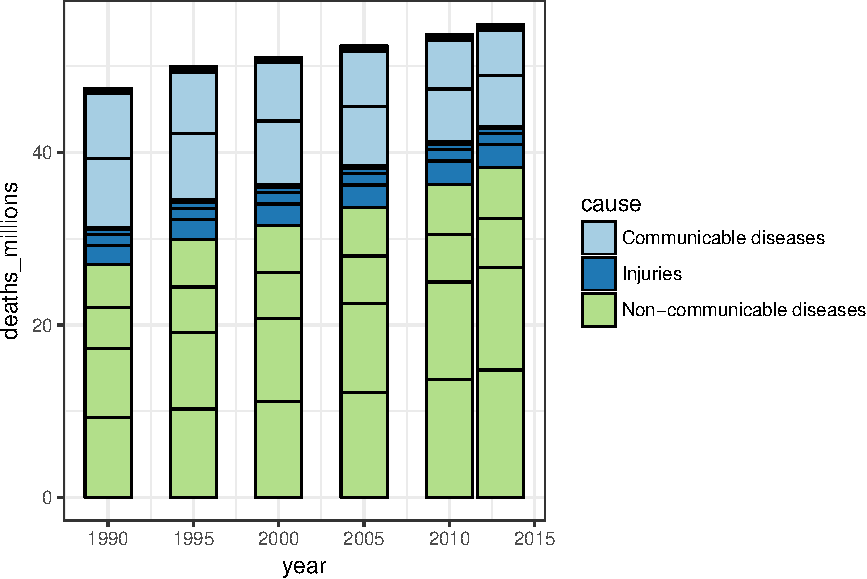
\includegraphics{03_summarising_files/figure-latex/unnamed-chunk-2-1.pdf}

\begin{Shaded}
\begin{Highlighting}[]
\NormalTok{mydata }\OperatorTok\StringTok{ }
\StringTok{    }\KeywordTok{filter}\NormalTok{(year }\OperatorTok{==}\StringTok{ }\DecValTok{1990}\NormalTok{)}
\end{Highlighting}
\end{Shaded}

\begin{verbatim}
##      location                     cause    sex year deaths_millions
## 1  Developing Non-communicable diseases   Male 1990       9.2277141
## 2  Developing Non-communicable diseases Female 1990       8.0242455
## 3   Developed Non-communicable diseases   Male 1990       4.7692902
## 4   Developed Non-communicable diseases Female 1990       4.9722431
## 5  Developing                  Injuries   Male 1990       2.2039625
## 6  Developing                  Injuries Female 1990       1.2698308
## 7   Developed                  Injuries   Male 1990       0.5941184
## 8   Developed                  Injuries Female 1990       0.2578759
## 9  Developing     Communicable diseases   Male 1990       7.9819728
## 10 Developing     Communicable diseases Female 1990       7.5416376
## 11  Developed     Communicable diseases   Male 1990       0.3387820
## 12  Developed     Communicable diseases Female 1990       0.2870169
\end{verbatim}

\section{Tidyverse packages: ggplot2, dplyr, tidyr,
etc.}\label{tidyverse-packages-ggplot2-dplyr-tidyr-etc.}

Most of the functions introduced in this session come from the tidyverse
family (\url{http://tidyverse.org/}), rather than Base R. Including
\texttt{library(tidyverse)} in your script loads a list of packages:
ggplot2, dplyr, tidry, forcats, etc.

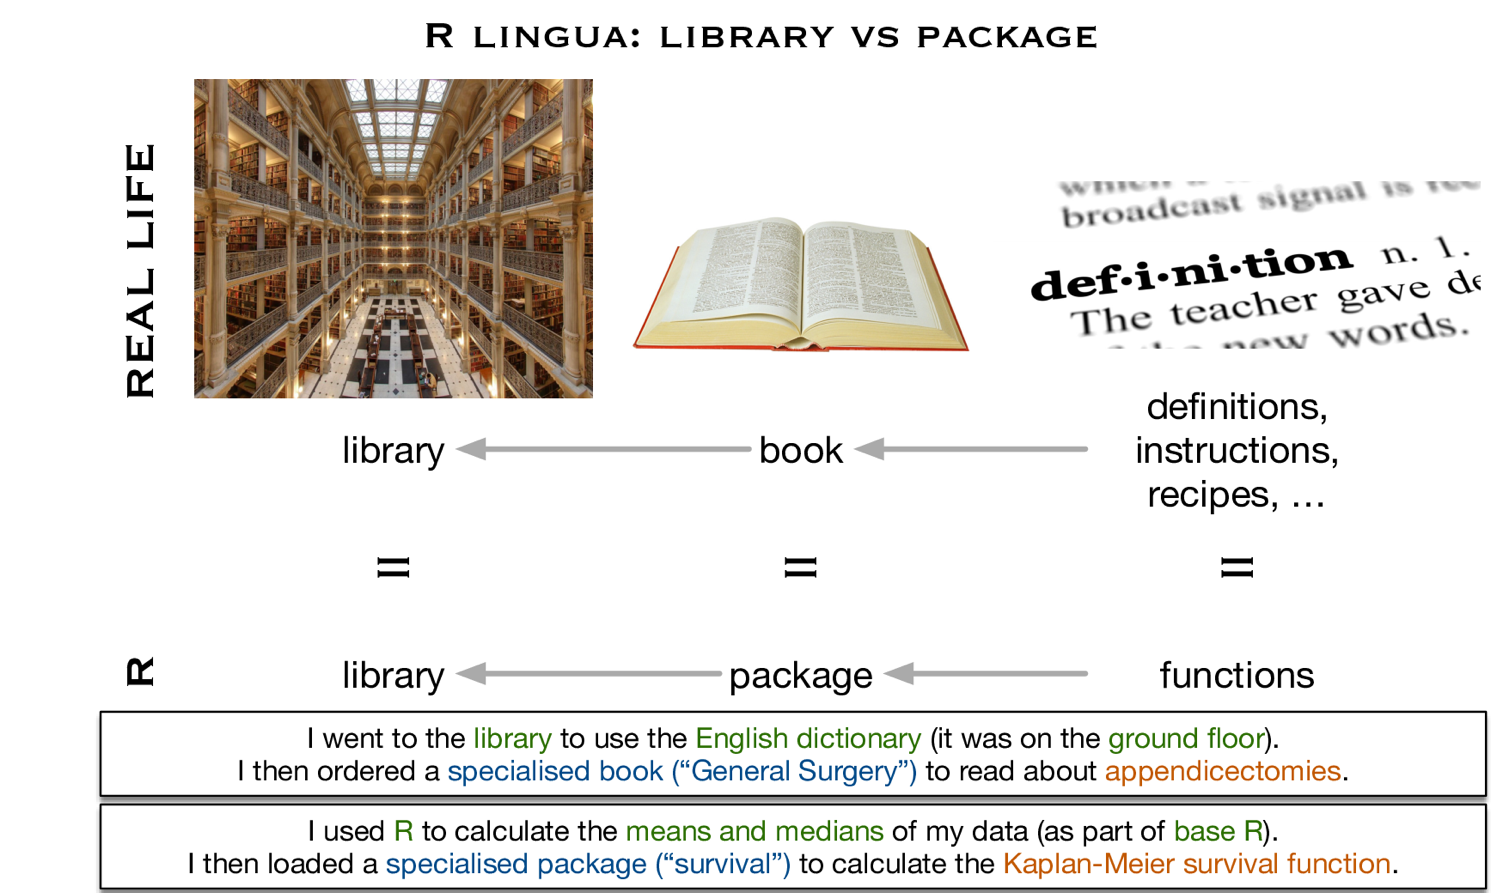
\includegraphics[width=20.71in]{images/library_vs_package}

\begin{Shaded}
\begin{Highlighting}[]
\KeywordTok{library}\NormalTok{(tidyverse)}
\end{Highlighting}
\end{Shaded}

\section{Basic functions for summarising
data}\label{basic-functions-for-summarising-data}

You can always pick a column and ask R to give you the \texttt{sum()},
\texttt{mean()}, \texttt{min()}, \texttt{max()}, etc. for it:

\begin{Shaded}
\begin{Highlighting}[]
\NormalTok{mydata}\OperatorTok{$}\NormalTok{deaths_millions }\OperatorTok\StringTok{ }\KeywordTok{sum}\NormalTok{()}
\end{Highlighting}
\end{Shaded}

\begin{verbatim}
## [1] 309.4174
\end{verbatim}

\begin{Shaded}
\begin{Highlighting}[]
\NormalTok{mydata}\OperatorTok{$}\NormalTok{deaths_millions }\OperatorTok\StringTok{ }\KeywordTok{mean}\NormalTok{()}
\end{Highlighting}
\end{Shaded}

\begin{verbatim}
## [1] 4.297463
\end{verbatim}

But if you want to get the total number of deaths for each \texttt{year}
(or \texttt{cause}, or \texttt{sex}, whichever grouping variables you
have in your dataset) you can use \texttt{group\_by()} and
\texttt{summarise()} that make subgroup analysis very convenient and
efficient.

\section{\texorpdfstring{Subgroup analysis: \texttt{group\_by()} and
\texttt{summarise()}}{Subgroup analysis: group\_by() and summarise()}}\label{subgroup-analysis-group_by-and-summarise}

The \texttt{group\_by()} function tells R that you are about to perform
subgroup analysis on your data. It retains information about your
groupings and calculations are applied on each group separately. To go
back to summarising the whole dataset again use \texttt{ungroup()}. Note
that \texttt{summarise()} is different to the \texttt{summary()}
function we used in Session 2.

With \texttt{summarise()}, we can calculate the total number of deaths
per year:

\begin{Shaded}
\begin{Highlighting}[]
\NormalTok{mydata }\OperatorTok\StringTok{ }
\StringTok{    }\KeywordTok{group_by}\NormalTok{(year) }\OperatorTok\StringTok{ }
\StringTok{    }\KeywordTok{summarise}\NormalTok{(}\DataTypeTok{total_per_year =} \KeywordTok{sum}\NormalTok{(deaths_millions)) ->}
\StringTok{    }\NormalTok{summary_data1}


\NormalTok{mydata }\OperatorTok\StringTok{ }
\StringTok{    }\KeywordTok{group_by}\NormalTok{(year, cause) }\OperatorTok\StringTok{ }
\StringTok{    }\KeywordTok{summarise}\NormalTok{(}\DataTypeTok{total_per_cause =} \KeywordTok{sum}\NormalTok{(deaths_millions)) ->}
\StringTok{    }\NormalTok{summary_data2}
\end{Highlighting}
\end{Shaded}

\begin{itemize}
\tightlist
\item
  \texttt{summary\_data1} includes the total number of deaths per year.
\item
  \texttt{summary\_data2} includes the number of deaths per cause per
  year.
\end{itemize}

\subsection{Exercise}\label{exercise-16}

Compare the sizes - number of rows (observations) and number of columns
(variables) - of \texttt{mydata}, \texttt{summary\_data1}, and
\texttt{summary\_data2} (in the Environment tab).

\begin{itemize}
\tightlist
\item
  \texttt{summary\_data2} has exactly 3 times as many rows as
  \texttt{summary\_data1}. Why?
\item
  \texttt{mydata} has 5 variables, whereas the summarised dataframes
  have 2 and 3. Which variables got dropped? Why?
\end{itemize}

\subsection{Exercise}\label{exercise-17}

For each cause, calculate its percentage to total deaths in each year.

Hint: Use \texttt{full\_join()} on \texttt{summary\_data1} and
\texttt{summary\_data2}.

Solution:

\begin{Shaded}
\begin{Highlighting}[]
\NormalTok{alldata =}\StringTok{ }\KeywordTok{full_join}\NormalTok{(summary_data1, summary_data2)}
\end{Highlighting}
\end{Shaded}

\begin{verbatim}
## Joining, by = "year"
\end{verbatim}

\begin{Shaded}
\begin{Highlighting}[]
\NormalTok{alldata}\OperatorTok{$}\NormalTok{percentage =}\StringTok{ }\KeywordTok{round}\NormalTok{(}\DecValTok{100}\OperatorTok{*}\NormalTok{alldata}\OperatorTok{$}\NormalTok{total_per_cause}\OperatorTok{/}\NormalTok{alldata}\OperatorTok{$}\NormalTok{total_per_year, }\DecValTok{0}\NormalTok{)}
\end{Highlighting}
\end{Shaded}

\section{\texorpdfstring{\texttt{mutate()}}{mutate()}}\label{mutate}

Mutate works similarly to \texttt{summarise()} (as in it respects
groupings set with \texttt{group\_by()}), but it adds a new column into
the original data. \texttt{summarise()}, on the other hand, condenses
the data into a minimal table that only includes the variables
specifically asked for.

\subsection{Exercise}\label{exercise-18}

Investigate these examples to learn how \texttt{summarise()} and
\texttt{mutate()} differ.

\begin{Shaded}
\begin{Highlighting}[]
\NormalTok{summarise_example =}\StringTok{ }\NormalTok{mydata }\OperatorTok\StringTok{ }
\StringTok{    }\KeywordTok{summarise}\NormalTok{(}\DataTypeTok{total_deaths =} \KeywordTok{sum}\NormalTok{(deaths_millions)) }

\NormalTok{mutate_example =}\StringTok{ }\NormalTok{mydata }\OperatorTok\StringTok{ }
\StringTok{    }\KeywordTok{mutate}\NormalTok{(}\DataTypeTok{total_deaths =} \KeywordTok{sum}\NormalTok{(deaths_millions))}
\end{Highlighting}
\end{Shaded}

You should see that \texttt{mutate()} adds the same number total number
(309.4174) to every line in the dataframe.

\subsection{Optional advanced
exercise}\label{optional-advanced-exercise}

Based on what we just observed on how \texttt{mutate()} adds a value to
each row, can you think of a way to redo \textbf{Exercise 3.4.2} without
using a join? Hint: instead of creating \texttt{summary\_data1} (total
deaths per year) as a separate dataframe which we then merge with
\texttt{summary\_data2} (total deaths for all causes per year), we can
use \texttt{mutate()} to add total death per year to each row.

\begin{Shaded}
\begin{Highlighting}[]
\NormalTok{mydata }\OperatorTok\StringTok{ }
\StringTok{    }\KeywordTok{group_by}\NormalTok{(year, cause) }\OperatorTok\StringTok{ }
\StringTok{    }\KeywordTok{summarise}\NormalTok{(}\DataTypeTok{total_per_cause =} \KeywordTok{sum}\NormalTok{(deaths_millions)) }\OperatorTok\StringTok{ }
\StringTok{    }\KeywordTok{group_by}\NormalTok{(year) }\OperatorTok\StringTok{ }
\StringTok{    }\KeywordTok{mutate}\NormalTok{(}\DataTypeTok{total_per_year =} \KeywordTok{sum}\NormalTok{(total_per_cause)) }\OperatorTok\StringTok{ }
\StringTok{    }\KeywordTok{mutate}\NormalTok{(}\DataTypeTok{percentage =} \DecValTok{100}\OperatorTok{*}\NormalTok{total_per_cause}\OperatorTok{/}\NormalTok{total_per_year) ->}\StringTok{ }\NormalTok{alldata}
\end{Highlighting}
\end{Shaded}

\section{\texorpdfstring{Wide vs long: \texttt{spread()} and
\texttt{gather()}}{Wide vs long: spread() and gather()}}\label{wide-vs-long-spread-and-gather}

\subsection{Wide format}\label{wide-format}

Although having data in the long format is very convenient for R, for
publication tables, it makes sense to spread some of the values out into
columns:

\begin{Shaded}
\begin{Highlighting}[]
\NormalTok{alldata }\OperatorTok
\StringTok{    }\KeywordTok{mutate}\NormalTok{(}\DataTypeTok{percentage =} \KeywordTok{paste0}\NormalTok{(}\KeywordTok{round}\NormalTok{(percentage, }\DecValTok{2}\NormalTok{), }\StringTok{"%"}\NormalTok{)) }\OperatorTok\StringTok{ }\CommentTok{#add a % label and round to 2 decimals}
\StringTok{    }\KeywordTok{select}\NormalTok{(year, cause, percentage) }\OperatorTok\StringTok{ }\CommentTok{#only select the variables you want in your final table}
\StringTok{    }\KeywordTok{spread}\NormalTok{(cause, percentage)}
\end{Highlighting}
\end{Shaded}

\begin{verbatim}
## # A tibble: 6 x 4
## # Groups:   year [6]
##    year `Communicable diseases` Injuries `Non-communicable diseases`
## * <int>                   <chr>    <chr>                       <chr>
## 1  1990                  34.02%    9.11%                      56.87%
## 2  1995                  30.91%    9.28%                      59.81%
## 3  2000                  28.93%    9.35%                      61.72%
## 4  2005                  26.53%    9.23%                      64.24%
## 5  2010                  23.17%    9.26%                      67.57%
## 6  2013                  21.53%    8.73%                      69.75%
\end{verbatim}

\subsection{Exercise}\label{exercise-19}

Calculate the percentage of male and female deaths for each year. Spread
it to a human readable form:

Hints:

\begin{itemize}
\tightlist
\item
  create \texttt{summary\_data3} that includes a variable called
  \texttt{total\_per\_sex}
\item
  merge \texttt{summary\_data1} and \texttt{summary\_data3} into a new
  data frame
\item
  calculate the percentage of \texttt{total\_per\_sex} to
  \texttt{total\_per\_year}
\item
  round, add \% labels
\item
  spread
\end{itemize}

Solution:

\begin{Shaded}
\begin{Highlighting}[]
\NormalTok{mydata }\OperatorTok\StringTok{ }
\StringTok{    }\KeywordTok{group_by}\NormalTok{(year) }\OperatorTok\StringTok{ }
\StringTok{    }\KeywordTok{summarise}\NormalTok{(}\DataTypeTok{total_per_year =} \KeywordTok{sum}\NormalTok{(deaths_millions)) ->}
\StringTok{    }\NormalTok{summary_data1}

\NormalTok{mydata }\OperatorTok\StringTok{ }
\StringTok{    }\KeywordTok{group_by}\NormalTok{(year, sex) }\OperatorTok\StringTok{ }
\StringTok{    }\KeywordTok{summarise}\NormalTok{(}\DataTypeTok{total_per_sex =} \KeywordTok{sum}\NormalTok{(deaths_millions)) ->}
\StringTok{    }\NormalTok{summary_data3}

\NormalTok{alldata =}\StringTok{ }\KeywordTok{full_join}\NormalTok{(summary_data1, summary_data3)}
\end{Highlighting}
\end{Shaded}

\begin{verbatim}
## Joining, by = "year"
\end{verbatim}

\begin{Shaded}
\begin{Highlighting}[]
\NormalTok{result_spread =}\StringTok{ }\NormalTok{alldata }\OperatorTok\StringTok{ }
\StringTok{  }\KeywordTok{mutate}\NormalTok{(}\DataTypeTok{percentage =} \KeywordTok{round}\NormalTok{(}\DecValTok{100}\OperatorTok{*}\NormalTok{total_per_sex}\OperatorTok{/}\NormalTok{total_per_year, }\DecValTok{0}\NormalTok{)) }\OperatorTok
\StringTok{  }\KeywordTok{mutate}\NormalTok{(}\DataTypeTok{percentage =} \KeywordTok{paste0}\NormalTok{(percentage, }\StringTok{"%"}\NormalTok{)) }\OperatorTok\StringTok{ }
\StringTok{  }\KeywordTok{select}\NormalTok{(year, sex, percentage) }\OperatorTok\StringTok{ }
\StringTok{  }\KeywordTok{spread}\NormalTok{(sex, percentage)}

\NormalTok{result_spread}
\end{Highlighting}
\end{Shaded}

\begin{verbatim}
## # A tibble: 6 x 3
##    year Female  Male
## * <int>  <chr> <chr>
## 1  1990    47%   53%
## 2  1995    47%   53%
## 3  2000    46%   54%
## 4  2005    46%   54%
## 5  2010    46%   54%
## 6  2013    45%   55%
\end{verbatim}

And save it into a csv file using \texttt{write\_csv()}:

\begin{Shaded}
\begin{Highlighting}[]
\KeywordTok{write_csv}\NormalTok{(result_spread, }\StringTok{"gbd_genders_summarised.csv"}\NormalTok{)}
\end{Highlighting}
\end{Shaded}

You can open a csv file with Excel and copy the table into Word or
PowerPoint for presenting.

\subsection{Long format}\label{long-format}

The opposite of \texttt{spread()} is \texttt{gather()}:

\begin{itemize}
\tightlist
\item
  The first argument is a name for the column that will include columns
  gathered from the wide columns (in this example, \texttt{Male} and
  \texttt{Female} are gathered into \texttt{sex}).
\item
  The second argument is a name for the column that will include the
  values from the wide-format columns (the values from \texttt{Male} and
  \texttt{Female} are gathered into \texttt{percentage}).
\item
  Any columns that already are condensed (e.g.~year was in one column,
  not spread out like in the pre-course example) must be included with a
  negative (i.e. -year).
\end{itemize}

\begin{Shaded}
\begin{Highlighting}[]
\NormalTok{result_spread }\OperatorTok\StringTok{ }
\StringTok{  }\KeywordTok{gather}\NormalTok{(sex, percentage, }\OperatorTok{-}\NormalTok{year)}
\end{Highlighting}
\end{Shaded}

\begin{verbatim}
## # A tibble: 12 x 3
##     year    sex percentage
##    <int>  <chr>      <chr>
##  1  1990 Female        47%
##  2  1995 Female        47%
##  3  2000 Female        46%
##  4  2005 Female        46%
##  5  2010 Female        46%
##  6  2013 Female        45%
##  7  1990   Male        53%
##  8  1995   Male        53%
##  9  2000   Male        54%
## 10  2005   Male        54%
## 11  2010   Male        54%
## 12  2013   Male        55%
\end{verbatim}

\subsection{Exercise}\label{exercise-20}

Test what happens when you

\begin{itemize}
\tightlist
\item
  Change the order of sex and percentage:
\end{itemize}

\begin{Shaded}
\begin{Highlighting}[]
\NormalTok{result_spread }\OperatorTok\StringTok{ }
\StringTok{  }\KeywordTok{gather}\NormalTok{(percentage, sex, }\OperatorTok{-}\NormalTok{year)}
\end{Highlighting}
\end{Shaded}

Turns out in the above example, \texttt{percentage} and \texttt{sex}
were just label you assigned to the gathered columns. It could be
anything, e.g.:

\begin{Shaded}
\begin{Highlighting}[]
\NormalTok{result_spread }\OperatorTok\StringTok{ }
\StringTok{  }\KeywordTok{gather}\NormalTok{(look}\OperatorTok{-}\NormalTok{I}\OperatorTok{-}\NormalTok{gathered}\OperatorTok{-}\NormalTok{sex, values}\OperatorTok{-}\NormalTok{Are}\OperatorTok{-}\NormalTok{Here, }\OperatorTok{-}\NormalTok{year)}
\end{Highlighting}
\end{Shaded}

\begin{itemize}
\tightlist
\item
  What happens if we omit \texttt{-year}:
\end{itemize}

\begin{Shaded}
\begin{Highlighting}[]
\NormalTok{result_spread }\OperatorTok\StringTok{ }
\StringTok{  }\KeywordTok{gather}\NormalTok{(sex, percentage)}
\end{Highlighting}
\end{Shaded}

\texttt{-year} was telling R we don't want the year column to be
gathered together with Male and Female, we want to keep it as it is.

\section{\texorpdfstring{Sorting:
\texttt{arrange()}}{Sorting: arrange()}}\label{sorting-arrange}

To reorder data ascendingly or descendingly, \texttt{use\ arrange()}:

\begin{Shaded}
\begin{Highlighting}[]
\NormalTok{mydata }\OperatorTok\StringTok{ }
\StringTok{    }\KeywordTok{group_by}\NormalTok{(year) }\OperatorTok\StringTok{ }
\StringTok{    }\KeywordTok{summarise}\NormalTok{(}\DataTypeTok{total =} \KeywordTok{sum}\NormalTok{(deaths_millions))  }\OperatorTok
\StringTok{    }\KeywordTok{arrange}\NormalTok{(}\OperatorTok{-}\NormalTok{year) }\CommentTok{# reorder after summarise()}
\end{Highlighting}
\end{Shaded}

\newpage 

\section{Factor handling}\label{factor-handling}

We talked about the pros and cons of working with factors in Session 2.
Overall, they are very useful for the type of analyses involved in
medical research.

\subsection{Exercise}\label{exercise-21}

Explain how and why these two plots are different.

\begin{Shaded}
\begin{Highlighting}[]
\NormalTok{mydata }\OperatorTok\StringTok{                                   }
\StringTok{    }\KeywordTok{ggplot}\NormalTok{(}\KeywordTok{aes}\NormalTok{(}\DataTypeTok{x=}\NormalTok{year, }\DataTypeTok{y=}\NormalTok{deaths_millions, }\DataTypeTok{fill=}\NormalTok{cause))}\OperatorTok{+}\StringTok{  }
\StringTok{    }\KeywordTok{geom_col}\NormalTok{()}
\end{Highlighting}
\end{Shaded}

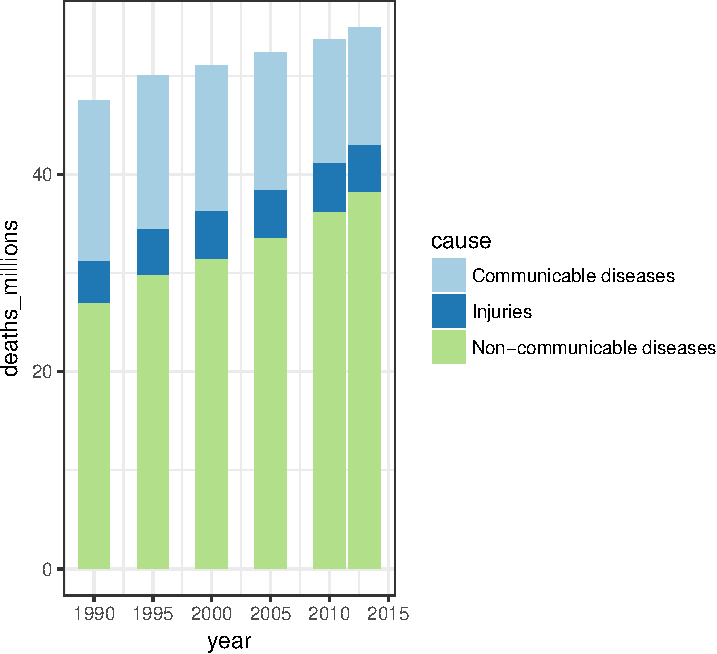
\includegraphics{03_summarising_files/figure-latex/unnamed-chunk-17-1.pdf}

\begin{Shaded}
\begin{Highlighting}[]
\NormalTok{mydata }\OperatorTok\StringTok{ }
\StringTok{    }\KeywordTok{ggplot}\NormalTok{(}\KeywordTok{aes}\NormalTok{(}\DataTypeTok{x=}\KeywordTok{factor}\NormalTok{(year), }\DataTypeTok{y=}\NormalTok{deaths_millions, }\DataTypeTok{fill=}\NormalTok{cause, }\DataTypeTok{colour=}\NormalTok{cause))}\OperatorTok{+}\StringTok{ }
\StringTok{    }\KeywordTok{geom_col}\NormalTok{()}
\end{Highlighting}
\end{Shaded}

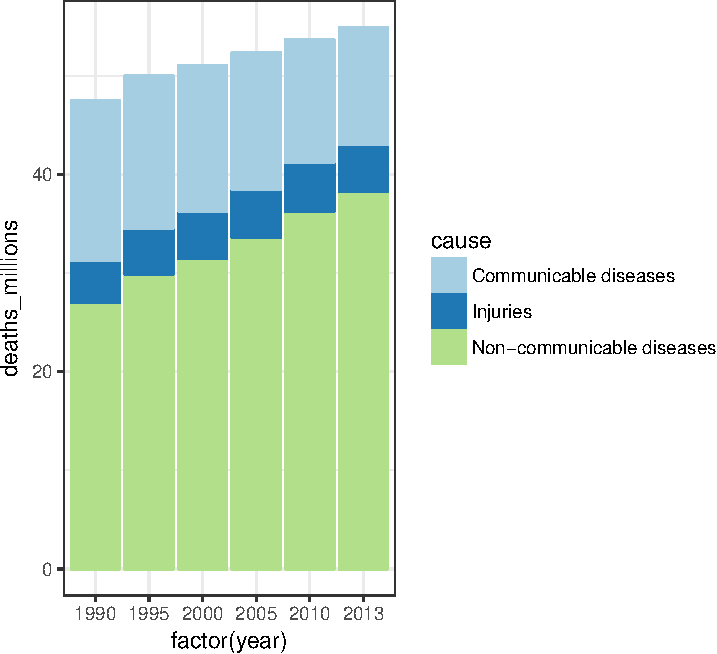
\includegraphics{03_summarising_files/figure-latex/unnamed-chunk-17-2.pdf}

What about these?

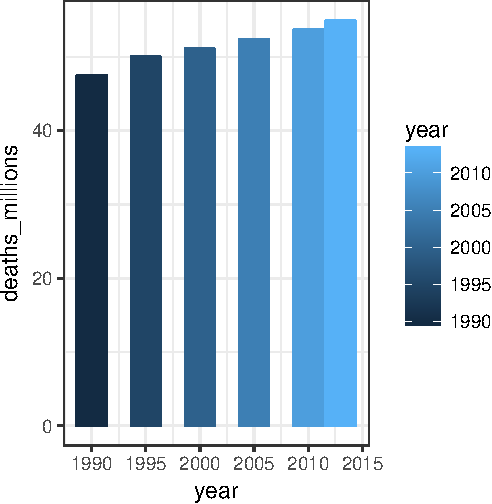
\includegraphics{03_summarising_files/figure-latex/unnamed-chunk-18-1.pdf}
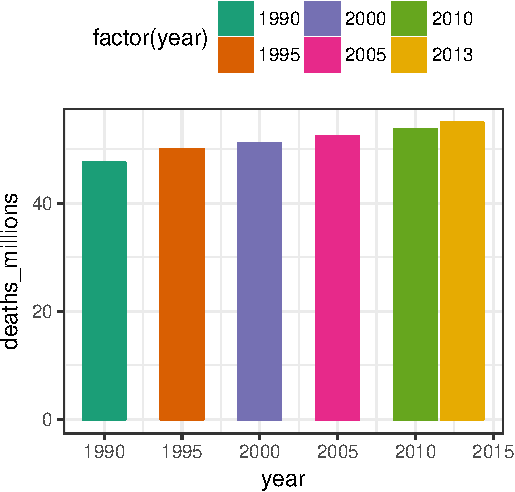
\includegraphics{03_summarising_files/figure-latex/unnamed-chunk-18-2.pdf}

These illustrate why it might sometimes be useful to use numbers as
factors - on the second one we have used \texttt{fill=factor(year)} as
the fill, so each year gets a distinct colour, rather than a gradual
palette.

\subsection{\texorpdfstring{\texttt{fct\_collapse()} - grouping levels
together}{fct\_collapse() - grouping levels together}}\label{fct_collapse---grouping-levels-together}

\begin{Shaded}
\begin{Highlighting}[]
\NormalTok{mydata}\OperatorTok{$}\NormalTok{cause  }\OperatorTok\StringTok{ }
\StringTok{    }\KeywordTok{fct_collapse}\NormalTok{(}\StringTok{"Non-communicable and injuries"}\NormalTok{ =}\StringTok{ }\KeywordTok{c}\NormalTok{(}\StringTok{"Non-communicable diseases"}\NormalTok{, }\StringTok{"Injuries"}\NormalTok{)) ->}
\StringTok{    }\NormalTok{mydata}\OperatorTok{$}\NormalTok{cause2}

\NormalTok{mydata}\OperatorTok{$}\NormalTok{cause }\OperatorTok\StringTok{ }\KeywordTok{levels}\NormalTok{()}
\end{Highlighting}
\end{Shaded}

\begin{verbatim}
## [1] "Communicable diseases"     "Injuries"                 
## [3] "Non-communicable diseases"
\end{verbatim}

\begin{Shaded}
\begin{Highlighting}[]
\NormalTok{mydata}\OperatorTok{$}\NormalTok{cause2 }\OperatorTok\StringTok{ }\KeywordTok{levels}\NormalTok{()}
\end{Highlighting}
\end{Shaded}

\begin{verbatim}
## [1] "Communicable diseases"         "Non-communicable and injuries"
\end{verbatim}

\subsection{\texorpdfstring{\texttt{fct\_relevel()} - change the order
of
levels}{fct\_relevel() - change the order of levels}}\label{fct_relevel---change-the-order-of-levels}

Another reason to sometimes make a numeric variable into a factor is
that we can then reorder it for the plot:

\begin{Shaded}
\begin{Highlighting}[]
\NormalTok{mydata}\OperatorTok{$}\NormalTok{year }\OperatorTok\StringTok{ }
\StringTok{  }\KeywordTok{factor}\NormalTok{() }\OperatorTok\StringTok{ }
\StringTok{    }\KeywordTok{fct_relevel}\NormalTok{(}\StringTok{"2013"}\NormalTok{) ->}\StringTok{ }\CommentTok{#brings 2013 to the front}
\StringTok{    }\NormalTok{mydata}\OperatorTok{$}\NormalTok{year.factor}

\KeywordTok{source}\NormalTok{(}\StringTok{"1_source_theme.R"}\NormalTok{)}

\NormalTok{mydata }\OperatorTok\StringTok{ }
\StringTok{    }\KeywordTok{ggplot}\NormalTok{(}\KeywordTok{aes}\NormalTok{(}\DataTypeTok{x=}\NormalTok{year.factor, }\DataTypeTok{y=}\NormalTok{deaths_millions, }\DataTypeTok{fill=}\NormalTok{cause))}\OperatorTok{+}\StringTok{ }
\StringTok{    }\KeywordTok{geom_col}\NormalTok{()}
\end{Highlighting}
\end{Shaded}

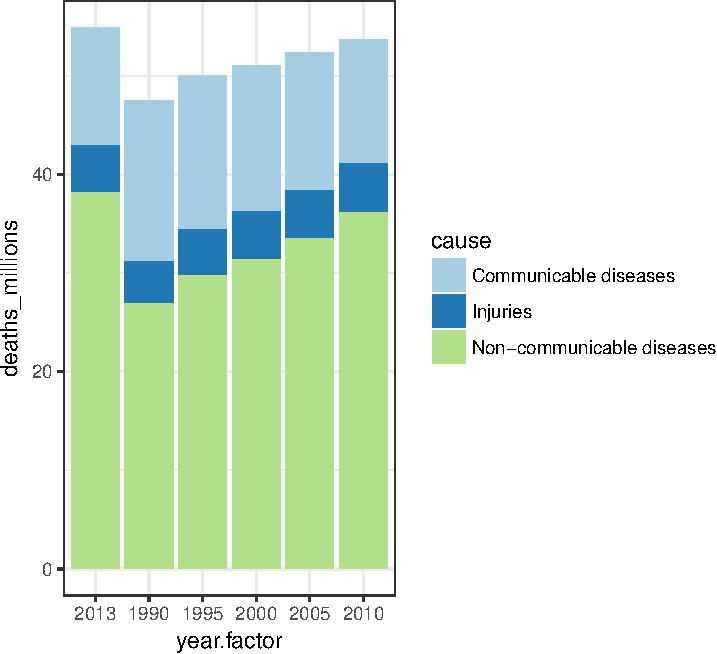
\includegraphics{03_summarising_files/figure-latex/unnamed-chunk-20-1.pdf}

\subsection{\texorpdfstring{\texttt{fct\_recode()} - rename
levels}{fct\_recode() - rename levels}}\label{fct_recode---rename-levels}

\begin{Shaded}
\begin{Highlighting}[]
\NormalTok{mydata}\OperatorTok{$}\NormalTok{cause }\OperatorTok\StringTok{ }
\StringTok{    }\KeywordTok{levels}\NormalTok{()  }\CommentTok{# levels() lists the factor levels of a column}
\end{Highlighting}
\end{Shaded}

\begin{verbatim}
## [1] "Communicable diseases"     "Injuries"                 
## [3] "Non-communicable diseases"
\end{verbatim}

\begin{Shaded}
\begin{Highlighting}[]
\NormalTok{mydata}\OperatorTok{$}\NormalTok{cause }\OperatorTok\StringTok{ }
\StringTok{    }\KeywordTok{fct_recode}\NormalTok{(}\StringTok{"Deaths from injury"}\NormalTok{ =}\StringTok{ "Injuries"}\NormalTok{) }\OperatorTok\StringTok{ }
\StringTok{    }\KeywordTok{levels}\NormalTok{()}
\end{Highlighting}
\end{Shaded}

\begin{verbatim}
## [1] "Communicable diseases"     "Deaths from injury"       
## [3] "Non-communicable diseases"
\end{verbatim}

\subsection{Converting factors to
numbers}\label{converting-factors-to-numbers}

MUST REMEMBER: factor needs to become \texttt{as.character()} before
converting to numeric or date! (Factors are actually stored as labelled
integers (so like number codes), only the function
\texttt{as.character()} will turn a factor back into a collated format
which can then be converted into a number or date.)

\subsection{Exercise}\label{exercise-22}

Investigate the two examples converting the \texttt{year.factor}
variable back to a number.

\begin{Shaded}
\begin{Highlighting}[]
\NormalTok{mydata}\OperatorTok{$}\NormalTok{year.factor}
\end{Highlighting}
\end{Shaded}

\begin{verbatim}
##  [1] 1990 1990 1990 1990 1995 1995 1995 1995 2000 2000 2000 2000 2005 2005
## [15] 2005 2005 2010 2010 2010 2010 2013 2013 2013 2013 1990 1990 1990 1990
## [29] 1995 1995 1995 1995 2000 2000 2000 2000 2005 2005 2005 2005 2010 2010
## [43] 2010 2010 2013 2013 2013 2013 1990 1990 1990 1990 1995 1995 1995 1995
## [57] 2000 2000 2000 2000 2005 2005 2005 2005 2010 2010 2010 2010 2013 2013
## [71] 2013 2013
## Levels: 2013 1990 1995 2000 2005 2010
\end{verbatim}

\begin{Shaded}
\begin{Highlighting}[]
\NormalTok{mydata}\OperatorTok{$}\NormalTok{year.factor }\OperatorTok
\StringTok{    }\KeywordTok{as.numeric}\NormalTok{()}
\end{Highlighting}
\end{Shaded}

\begin{verbatim}
##  [1] 2 2 2 2 3 3 3 3 4 4 4 4 5 5 5 5 6 6 6 6 1 1 1 1 2 2 2 2 3 3 3 3 4 4 4
## [36] 4 5 5 5 5 6 6 6 6 1 1 1 1 2 2 2 2 3 3 3 3 4 4 4 4 5 5 5 5 6 6 6 6 1 1
## [71] 1 1
\end{verbatim}

\begin{Shaded}
\begin{Highlighting}[]
\NormalTok{mydata}\OperatorTok{$}\NormalTok{year.factor }\OperatorTok
\StringTok{    }\KeywordTok{as.character}\NormalTok{() }\OperatorTok\StringTok{ }
\StringTok{    }\KeywordTok{as.numeric}\NormalTok{()}
\end{Highlighting}
\end{Shaded}

\begin{verbatim}
##  [1] 1990 1990 1990 1990 1995 1995 1995 1995 2000 2000 2000 2000 2005 2005
## [15] 2005 2005 2010 2010 2010 2010 2013 2013 2013 2013 1990 1990 1990 1990
## [29] 1995 1995 1995 1995 2000 2000 2000 2000 2005 2005 2005 2005 2010 2010
## [43] 2010 2010 2013 2013 2013 2013 1990 1990 1990 1990 1995 1995 1995 1995
## [57] 2000 2000 2000 2000 2005 2005 2005 2005 2010 2010 2010 2010 2013 2013
## [71] 2013 2013
\end{verbatim}

\newpage 

\section{Long Exercise}\label{long-exercise}

This exercise includes multiple steps, combining all of the above.

First, create a new script called ``2\_long\_exercise.R''. Then Restart
your R session, add \texttt{library(tidyverse)} and load
\texttt{"global\_burden\_disease\_long.rda"} again.

\begin{itemize}
\tightlist
\item
  Calculate the total number of deaths in Developed and Developing
  countries. Hint: use \texttt{group\_by(location)} and
  \texttt{summarise(\ Include\ new\ column\ name\ =\ sum()\ here)}.
\item
  Calculate the total number of deaths in Developed and Developing
  countries and for men and women. Hint: this is as easy as adding
  \texttt{,\ sex} to \texttt{group\_by()}.
\item
  Filter for 1990.
\item
  \texttt{spread()} the the \texttt{location} column.
\end{itemize}

\begin{verbatim}
## # A tibble: 2 x 3
##      sex Developed Developing
## * <fctr>     <dbl>      <dbl>
## 1 Female  5.517136   16.83571
## 2   Male  5.702191   19.41365
\end{verbatim}

\section{Extra: formatting a table for
publication}\label{extra-formatting-a-table-for-publication}

Creating a publication table with both the total numbers and percentages
(in brackets) + using \texttt{formatC()} to retain trailing zeros:

\begin{Shaded}
\begin{Highlighting}[]
\CommentTok{# Let's use alldata from Exercise 5.2:}

\NormalTok{mydata }\OperatorTok\StringTok{ }
\StringTok{    }\KeywordTok{group_by}\NormalTok{(year, cause) }\OperatorTok\StringTok{ }
\StringTok{    }\KeywordTok{summarise}\NormalTok{(}\DataTypeTok{total_per_cause =} \KeywordTok{sum}\NormalTok{(deaths_millions)) }\OperatorTok\StringTok{ }
\StringTok{    }\KeywordTok{group_by}\NormalTok{(year) }\OperatorTok\StringTok{ }
\StringTok{    }\KeywordTok{mutate}\NormalTok{(}\DataTypeTok{total_per_year =} \KeywordTok{sum}\NormalTok{(total_per_cause)) }\OperatorTok\StringTok{ }
\StringTok{    }\KeywordTok{mutate}\NormalTok{(}\DataTypeTok{percentage =} \DecValTok{100}\OperatorTok{*}\NormalTok{total_per_cause}\OperatorTok{/}\NormalTok{total_per_year) ->}\StringTok{ }\NormalTok{alldata}

\NormalTok{alldata }\OperatorTok
\StringTok{    }\KeywordTok{mutate}\NormalTok{(}\DataTypeTok{total_percentage =}   
                    \KeywordTok{paste0}\NormalTok{(}\KeywordTok{round}\NormalTok{(total_per_cause, }\DecValTok{1}\NormalTok{)  }\OperatorTok\StringTok{ }\KeywordTok{formatC}\NormalTok{(}\DecValTok{1}\NormalTok{, }\DataTypeTok{format =} \StringTok{"f"}\NormalTok{),}
                           \StringTok{" ("}\NormalTok{, }\KeywordTok{round}\NormalTok{(percentage, }\DecValTok{1}\NormalTok{) }\OperatorTok\StringTok{ }\KeywordTok{formatC}\NormalTok{(}\DecValTok{1}\NormalTok{, }\DataTypeTok{format =} \StringTok{"f"}\NormalTok{),}
                           \StringTok{"%)"}
\NormalTok{                           )}
\NormalTok{                    ) }\OperatorTok
\StringTok{    }\KeywordTok{select}\NormalTok{(year, cause, total_percentage) }\OperatorTok
\StringTok{    }\KeywordTok{spread}\NormalTok{(cause, total_percentage)}
\end{Highlighting}
\end{Shaded}

\begin{verbatim}
## # A tibble: 6 x 4
## # Groups:   year [6]
##    year `Communicable diseases`   Injuries `Non-communicable diseases`
## * <int>                   <chr>      <chr>                       <chr>
## 1  1990            16.1 (34.0%) 4.3 (9.1%)                27.0 (56.9%)
## 2  1995            15.4 (30.9%) 4.6 (9.3%)                29.9 (59.8%)
## 3  2000            14.8 (28.9%) 4.8 (9.4%)                31.5 (61.7%)
## 4  2005            13.9 (26.5%) 4.8 (9.2%)                33.6 (64.2%)
## 5  2010            12.4 (23.2%) 5.0 (9.3%)                36.3 (67.6%)
## 6  2013            11.8 (21.5%) 4.8 (8.7%)                38.3 (69.7%)
\end{verbatim}

\section{Solution: Long Exercise}\label{solution-long-exercise}

\begin{Shaded}
\begin{Highlighting}[]
\NormalTok{mydata }\OperatorTok\StringTok{ }
\StringTok{  }\KeywordTok{filter}\NormalTok{(year }\OperatorTok{==}\StringTok{ }\DecValTok{1990}\NormalTok{) }\OperatorTok\StringTok{ }
\StringTok{  }\KeywordTok{group_by}\NormalTok{(location, sex) }\OperatorTok\StringTok{ }
\StringTok{  }\KeywordTok{summarise}\NormalTok{(}\DataTypeTok{total_deaths =} \KeywordTok{sum}\NormalTok{(deaths_millions)) }\OperatorTok\StringTok{ }
\StringTok{  }\KeywordTok{spread}\NormalTok{(location, total_deaths)}
\end{Highlighting}
\end{Shaded}

\chapter{Different types of plots}\label{different-types-of-plots}

\section{Data}\label{data-2}

We will be using the gapminder dataset:

\begin{Shaded}
\begin{Highlighting}[]
\KeywordTok{library}\NormalTok{(tidyverse)}
\KeywordTok{library}\NormalTok{(forcats)}
\KeywordTok{library}\NormalTok{(gapminder)}

\NormalTok{mydata =}\StringTok{ }\NormalTok{gapminder}

\KeywordTok{summary}\NormalTok{(mydata)}
\end{Highlighting}
\end{Shaded}

\begin{verbatim}
##         country        continent        year         lifeExp     
##  Afghanistan:  12   Africa  :624   Min.   :1952   Min.   :23.60  
##  Albania    :  12   Americas:300   1st Qu.:1966   1st Qu.:48.20  
##  Algeria    :  12   Asia    :396   Median :1980   Median :60.71  
##  Angola     :  12   Europe  :360   Mean   :1980   Mean   :59.47  
##  Argentina  :  12   Oceania : 24   3rd Qu.:1993   3rd Qu.:70.85  
##  Australia  :  12                  Max.   :2007   Max.   :82.60  
##  (Other)    :1632                                                
##       pop              gdpPercap       
##  Min.   :6.001e+04   Min.   :   241.2  
##  1st Qu.:2.794e+06   1st Qu.:  1202.1  
##  Median :7.024e+06   Median :  3531.8  
##  Mean   :2.960e+07   Mean   :  7215.3  
##  3rd Qu.:1.959e+07   3rd Qu.:  9325.5  
##  Max.   :1.319e+09   Max.   :113523.1  
## 
\end{verbatim}

\begin{Shaded}
\begin{Highlighting}[]
\NormalTok{mydata}\OperatorTok{$}\NormalTok{year }\OperatorTok\StringTok{ }\KeywordTok{unique}\NormalTok{()}
\end{Highlighting}
\end{Shaded}

\begin{verbatim}
##  [1] 1952 1957 1962 1967 1972 1977 1982 1987 1992 1997 2002 2007
\end{verbatim}

\section{\texorpdfstring{Scatter plots/bubble plots -
\texttt{geom\_point()}}{Scatter plots/bubble plots - geom\_point()}}\label{scatter-plotsbubble-plots---geom_point}

Plot life expectancy against GDP per capita
(\texttt{x\ =\ gdpPercap,\ y=lifeExp}) at year 2007:

\begin{Shaded}
\begin{Highlighting}[]
\NormalTok{mydata }\OperatorTok\StringTok{ }
\StringTok{  }\KeywordTok{filter}\NormalTok{(year }\OperatorTok{==}\StringTok{ }\DecValTok{2007}\NormalTok{) }\OperatorTok\StringTok{ }
\StringTok{  }\KeywordTok{ggplot}\NormalTok{(}\KeywordTok{aes}\NormalTok{(}\DataTypeTok{x =}\NormalTok{ gdpPercap, }\DataTypeTok{y=}\NormalTok{lifeExp)) }\OperatorTok{+}
\StringTok{  }\KeywordTok{geom_point}\NormalTok{()}
\end{Highlighting}
\end{Shaded}

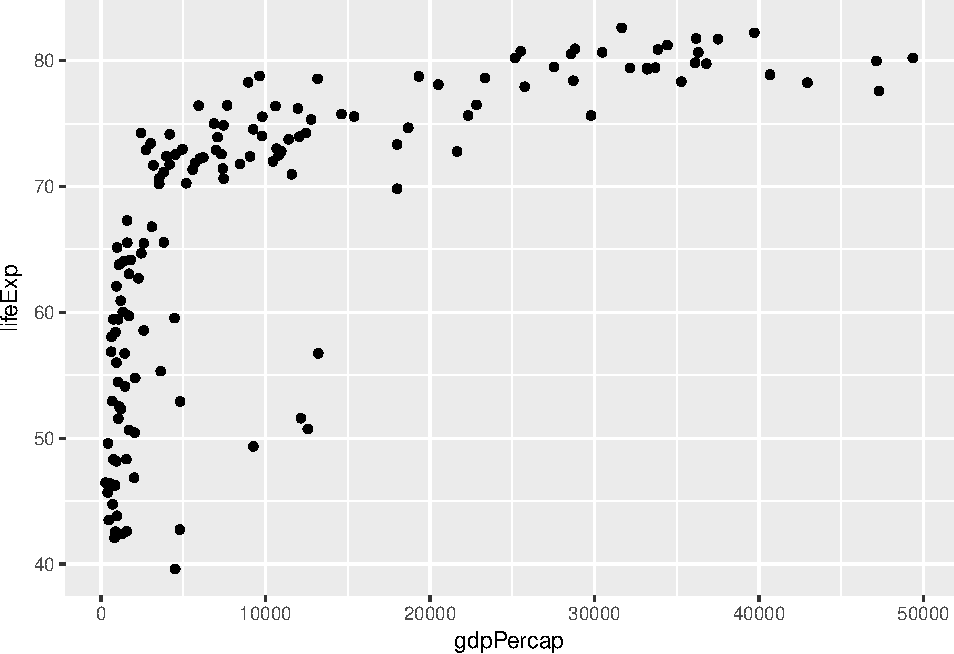
\includegraphics{04_plotting_files/figure-latex/unnamed-chunk-2-1.pdf}

\subsection{Exercise}\label{exercise-23}

Follow the step-by-step instructions to transform the grey plot just
above into this:

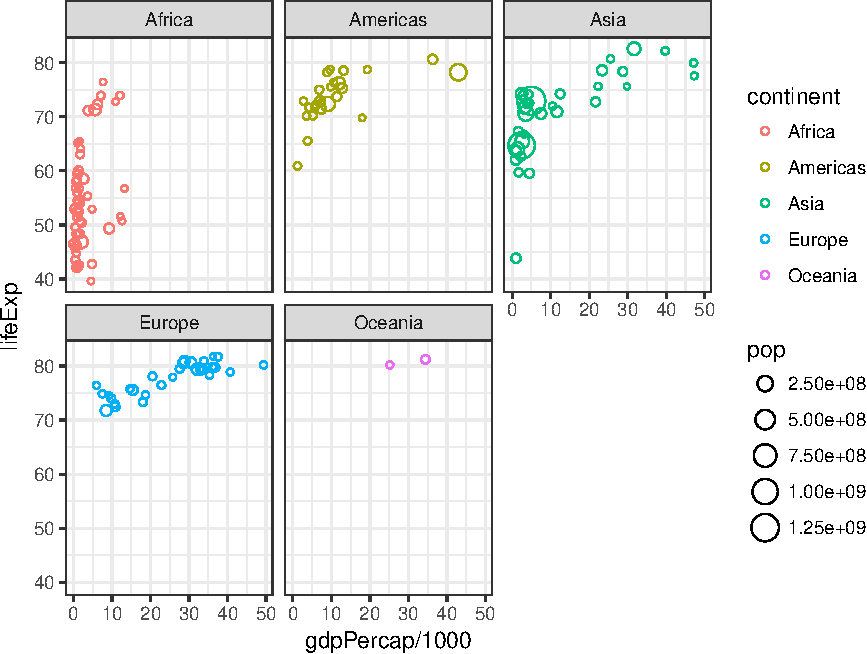
\includegraphics{04_plotting_files/figure-latex/unnamed-chunk-3-1.pdf}

\begin{itemize}
\tightlist
\item
  Add points: \texttt{geom\_point()}

  \begin{itemize}
  \tightlist
  \item
    Change point type: \texttt{shape\ =\ 1} (or any number from your
    Quickstart Sheet) inside the \texttt{geom\_point()}
  \end{itemize}
\item
  Colour each country point by its continent: \texttt{colour=continent}
  to aes()
\item
  Size each country point by its population: \texttt{size=pop} to aes()
\item
  Put the country points of each continent on a separate panel:
  \texttt{+\ facet\_wrap(\textasciitilde{}continent)}
\item
  Make the background white: \texttt{+\ theme\_bw()}
\end{itemize}

\section{\texorpdfstring{Line chart/timeplot -
\texttt{geom\_line()}}{Line chart/timeplot - geom\_line()}}\label{line-charttimeplot---geom_line}

Plot life expectancy against year (\texttt{x\ =\ year,\ y=lifeExp}), add
\texttt{geom\_line()}:

\begin{Shaded}
\begin{Highlighting}[]
\NormalTok{mydata }\OperatorTok\StringTok{ }
\StringTok{  }\KeywordTok{ggplot}\NormalTok{(}\KeywordTok{aes}\NormalTok{(}\DataTypeTok{x =}\NormalTok{ year, }\DataTypeTok{y=}\NormalTok{lifeExp)) }\OperatorTok{+}
\StringTok{  }\KeywordTok{geom_line}\NormalTok{()}
\end{Highlighting}
\end{Shaded}

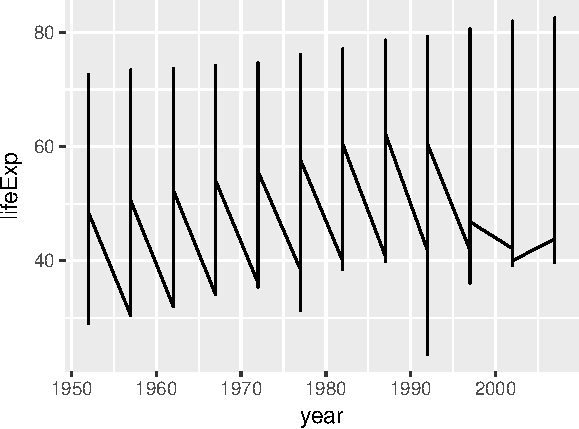
\includegraphics{04_plotting_files/figure-latex/unnamed-chunk-4-1.pdf}

The reason you now see this weird zig-zag is that, using the above code,
R does not know you want a connected line for each country. Specify how
you want data points grouped to lines: \texttt{group\ =\ country} in
\texttt{aes()}:

\begin{Shaded}
\begin{Highlighting}[]
\NormalTok{mydata }\OperatorTok\StringTok{ }
\StringTok{  }\KeywordTok{ggplot}\NormalTok{(}\KeywordTok{aes}\NormalTok{(}\DataTypeTok{x =}\NormalTok{ year, }\DataTypeTok{y=}\NormalTok{lifeExp, }\DataTypeTok{group =}\NormalTok{ country)) }\OperatorTok{+}
\StringTok{  }\KeywordTok{geom_line}\NormalTok{()}
\end{Highlighting}
\end{Shaded}

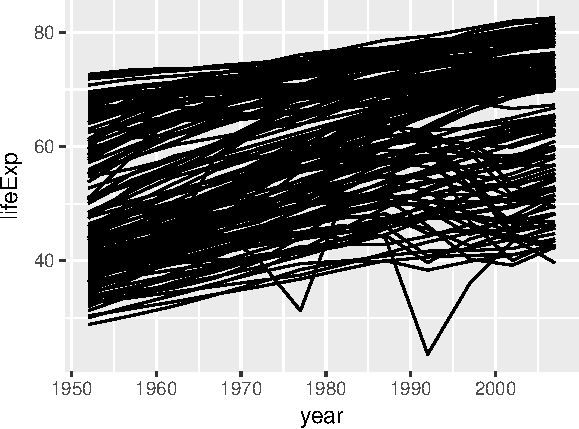
\includegraphics{04_plotting_files/figure-latex/unnamed-chunk-5-1.pdf}

\subsection{Exercise}\label{exercise-24}

Follow the step-by-step instructions to transform the grey plot just
above into this:

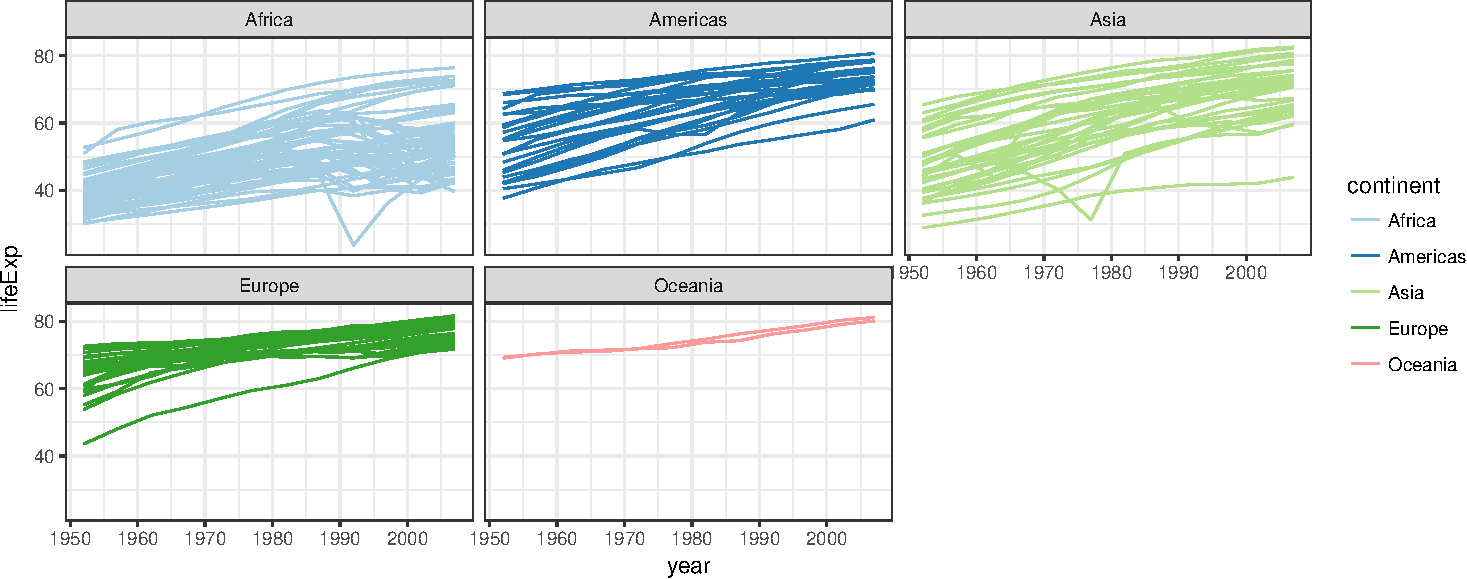
\includegraphics{04_plotting_files/figure-latex/unnamed-chunk-6-1.pdf}

\begin{itemize}
\tightlist
\item
  Colour lines by continents: \texttt{colour=continent} to
  \texttt{aes()}
\item
  \emph{Similarly to what we did in \texttt{geom\_point()}, you can even
  size the line thicknesses by each country's population:
  \texttt{size=pop} to \texttt{aes()}}
\item
  Continents on separate panels:
  \texttt{+\ facet\_wrap(\textasciitilde{}continent)}
\item
  Make the background white: \texttt{+\ theme\_bw()}
\item
  Use a nicer colour scheme:
  \texttt{+\ scale\_colour\_brewer(palette\ =\ "Paired")}
\end{itemize}

\subsection{Advanced example}\label{advanced-example}

For European countries only
(\texttt{filter(continent\ ==\ "Europe")\ \%\textgreater{}\%}), plot
life expectancy over time in grey colour for all countries, then add
United Kingdom as a red line:

\begin{Shaded}
\begin{Highlighting}[]
\NormalTok{mydata }\OperatorTok
\StringTok{  }\KeywordTok{filter}\NormalTok{(continent }\OperatorTok{==}\StringTok{ "Europe"}\NormalTok{) }\OperatorTok\StringTok{ }\CommentTok{#Europe only}
\StringTok{  }\KeywordTok{ggplot}\NormalTok{(}\KeywordTok{aes}\NormalTok{(}\DataTypeTok{x =}\NormalTok{ year, }\DataTypeTok{y=}\NormalTok{lifeExp, }\DataTypeTok{group =}\NormalTok{ country)) }\OperatorTok{+}
\StringTok{  }\KeywordTok{geom_line}\NormalTok{(}\DataTypeTok{colour =} \StringTok{"grey"}\NormalTok{) }\OperatorTok{+}
\StringTok{  }\KeywordTok{theme_bw}\NormalTok{() }\OperatorTok{+}
\StringTok{  }\KeywordTok{geom_line}\NormalTok{(}\DataTypeTok{data =} \KeywordTok{filter}\NormalTok{(mydata, country }\OperatorTok{==}\StringTok{ "United Kingdom"}\NormalTok{), }\DataTypeTok{colour =} \StringTok{"red"}\NormalTok{)}
\end{Highlighting}
\end{Shaded}

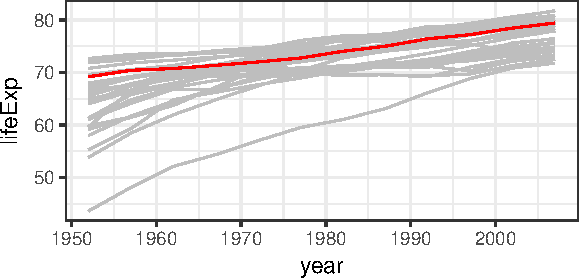
\includegraphics{04_plotting_files/figure-latex/unnamed-chunk-7-1.pdf}

\subsection{Advanced Exercise}\label{advanced-exercise}

As previous, but add a line for France in blue:

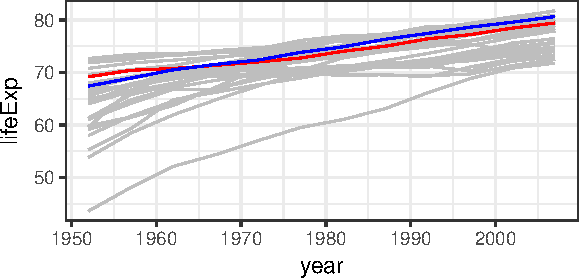
\includegraphics{04_plotting_files/figure-latex/unnamed-chunk-8-1.pdf}

\section{\texorpdfstring{Box-plot -
\texttt{geom\_boxplot()}}{Box-plot - geom\_boxplot()}}\label{box-plot---geom_boxplot}

Plot the distribution of life expectancies within each continent at year
2007:

\begin{itemize}
\tightlist
\item
  \texttt{filter(year\ ==\ 2007)\ \%\textgreater{}\%}
\item
  \texttt{x\ =\ continent,\ y\ =\ lifeExp}
\item
  \texttt{+\ geom\_boxplot()}
\end{itemize}

\begin{Shaded}
\begin{Highlighting}[]
\NormalTok{mydata }\OperatorTok\StringTok{ }
\StringTok{  }\KeywordTok{filter}\NormalTok{(year }\OperatorTok{==}\StringTok{ }\DecValTok{2007}\NormalTok{) }\OperatorTok\StringTok{ }
\StringTok{  }\KeywordTok{ggplot}\NormalTok{(}\KeywordTok{aes}\NormalTok{(}\DataTypeTok{x =}\NormalTok{ continent, }\DataTypeTok{y =}\NormalTok{ lifeExp)) }\OperatorTok{+}
\StringTok{  }\KeywordTok{geom_boxplot}\NormalTok{() }\OperatorTok{+}
\StringTok{  }\KeywordTok{theme_bw}\NormalTok{()}
\end{Highlighting}
\end{Shaded}

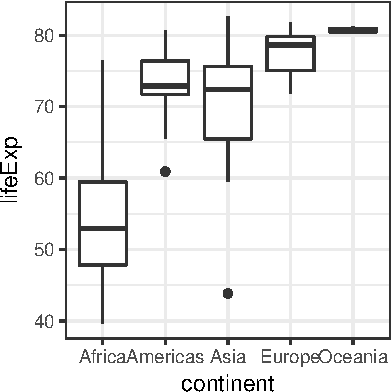
\includegraphics{04_plotting_files/figure-latex/unnamed-chunk-9-1.pdf}

\subsection{Exercise}\label{exercise-25}

Add individual (country) points on top of the box plot:

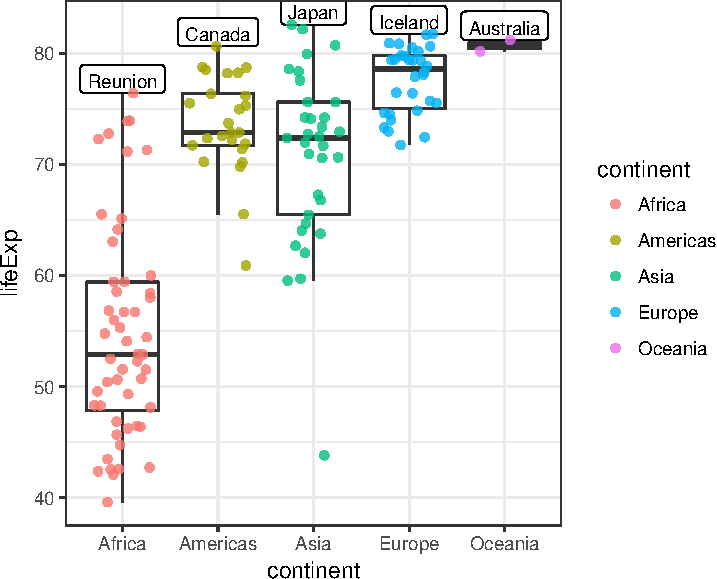
\includegraphics{04_plotting_files/figure-latex/unnamed-chunk-10-1.pdf}

Hint: Use \texttt{geom\_jitter()} instead of \texttt{geom\_point()} to
reduce overlap by spreading the points horizontally. Include the
\texttt{width=0.3} option to reduce the width of the jitter.

\textbf{Optional:}

Include text labels for the highest life expectancy country of each
continent.

\textbf{Hint 1} Create a separate dataframe called \texttt{label\_data}
with the maximum countries for each continent:

\begin{Shaded}
\begin{Highlighting}[]
\NormalTok{label_data =}\StringTok{ }\NormalTok{mydata }\OperatorTok\StringTok{ }
\StringTok{  }\KeywordTok{filter}\NormalTok{(year }\OperatorTok{==}\StringTok{ }\KeywordTok{max}\NormalTok{(year)) }\OperatorTok\StringTok{ }\CommentTok{# same as year == 2007}
\StringTok{  }\KeywordTok{group_by}\NormalTok{(continent) }\OperatorTok\StringTok{ }
\StringTok{  }\KeywordTok{filter}\NormalTok{(lifeExp }\OperatorTok{==}\StringTok{ }\KeywordTok{max}\NormalTok{(lifeExp) )}
\end{Highlighting}
\end{Shaded}

\textbf{Hint 2} Add \texttt{geom\_label()} with appropriate
\texttt{aes()}:

\begin{Shaded}
\begin{Highlighting}[]
\OperatorTok{+}\StringTok{ }\KeywordTok{geom_label}\NormalTok{(}\DataTypeTok{data =}\NormalTok{ label_data, }\KeywordTok{aes}\NormalTok{(}\DataTypeTok{label=}\NormalTok{country), }\DataTypeTok{vjust =} \DecValTok{0}\NormalTok{)}
\end{Highlighting}
\end{Shaded}

\subsection{\texorpdfstring{Dot-plot -
\texttt{geom\_dotplot()}}{Dot-plot - geom\_dotplot()}}\label{dot-plot---geom_dotplot}

\texttt{geom\_dotplot(aes(fill=continent),\ binaxis\ =\ \textquotesingle{}y\textquotesingle{},\ stackdir\ =\ \textquotesingle{}center\textquotesingle{},\ alpha=0.6)}

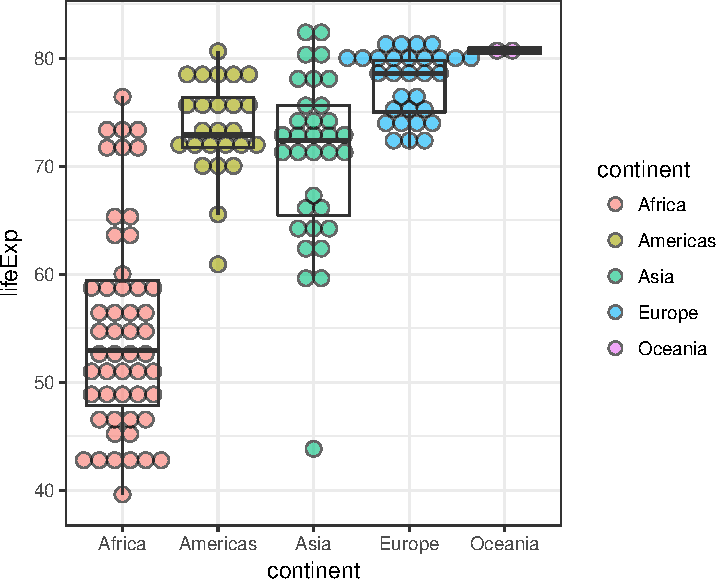
\includegraphics{04_plotting_files/figure-latex/unnamed-chunk-13-1.pdf}

\section{\texorpdfstring{Barplot - \texttt{geom\_bar()} and
\texttt{geom\_col()}}{Barplot - geom\_bar() and geom\_col()}}\label{barplot---geom_bar-and-geom_col}

In the first module, we plotted barplots from already summarised data
(using the \texttt{geom\_col}), but \texttt{geom\_bar()} is perfectly
happy to count up data for you. For example, we can plot the number of
countries in each continent without summarising the data beforehand:

\begin{Shaded}
\begin{Highlighting}[]
\NormalTok{mydata }\OperatorTok\StringTok{ }
\StringTok{  }\KeywordTok{filter}\NormalTok{(year }\OperatorTok{==}\StringTok{ }\DecValTok{2007}\NormalTok{) }\OperatorTok\StringTok{ }
\StringTok{  }\KeywordTok{ggplot}\NormalTok{(}\KeywordTok{aes}\NormalTok{(}\DataTypeTok{x =}\NormalTok{ continent)) }\OperatorTok{+}
\StringTok{  }\KeywordTok{geom_bar}\NormalTok{() }\OperatorTok{+}\StringTok{ }
\StringTok{  }\KeywordTok{ylab}\NormalTok{(}\StringTok{"Number of countries"}\NormalTok{) }\OperatorTok{+}
\StringTok{  }\KeywordTok{theme_bw}\NormalTok{()}
\end{Highlighting}
\end{Shaded}

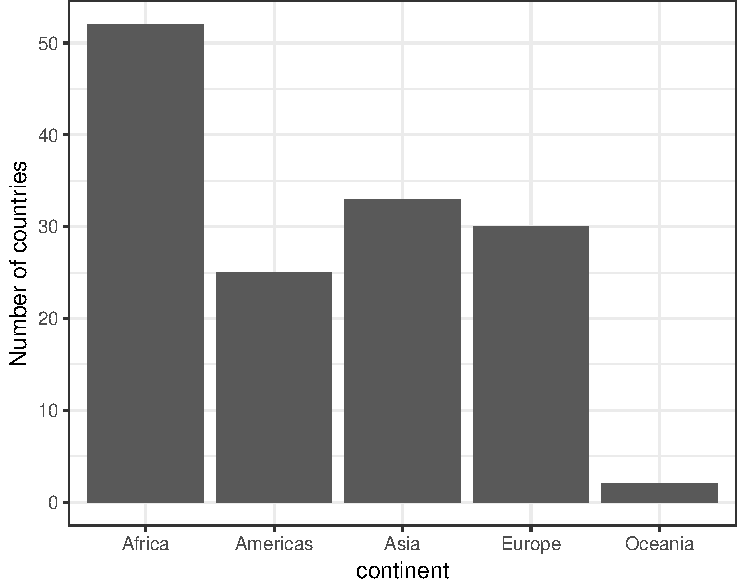
\includegraphics{04_plotting_files/figure-latex/unnamed-chunk-14-1.pdf}

\subsection{Exercise}\label{exercise-26}

Create this barplot of life expectancies in European countries (year
2007). Hint: \texttt{coord\_flip()} makes the bars horizontal,
\texttt{fill\ =\ NA} makes them empty, have a look at your QuickStar
sheet for different themes.

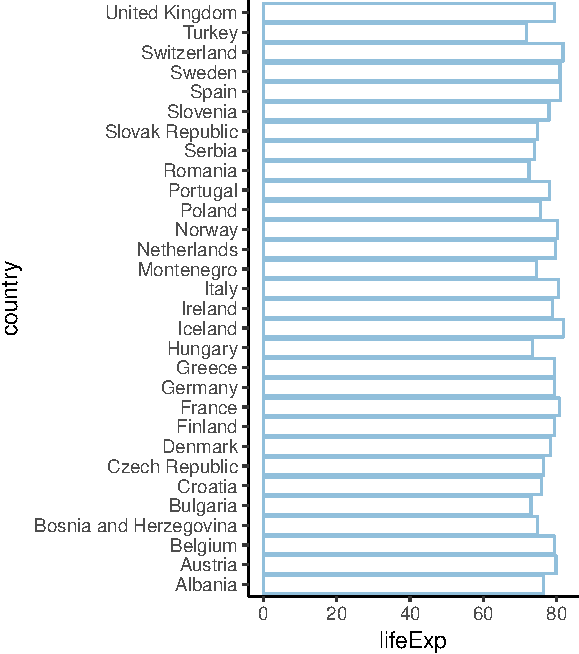
\includegraphics{04_plotting_files/figure-latex/unnamed-chunk-15-1.pdf}

\section{All other types of plots}\label{all-other-types-of-plots}

These are just some of the main ones, see this gallery for more options:
\url{http://www.r-graph-gallery.com/portfolio/ggplot2-package/}

And the \texttt{ggplot()} documentation: \url{http://docs.ggplot2.org/}

Remember that you can always combine different types of plots - i.e.~add
lines or points on bars, etc.

\section{\texorpdfstring{Specifying \texttt{aes()}
variables}{Specifying aes() variables}}\label{specifying-aes-variables}

The \texttt{aes()} variables wrapped inside \texttt{ggplot()} will be
taken into account by all geoms. If you put
\texttt{aes(colour\ =\ lifeExp)} inside \texttt{geom\_point()}, only
points will be coloured:

\begin{Shaded}
\begin{Highlighting}[]
\NormalTok{mydata }\OperatorTok\StringTok{ }
\StringTok{  }\KeywordTok{filter}\NormalTok{(continent }\OperatorTok{==}\StringTok{ "Europe"}\NormalTok{) }\OperatorTok\StringTok{ }
\StringTok{  }\KeywordTok{ggplot}\NormalTok{(}\KeywordTok{aes}\NormalTok{(}\DataTypeTok{x =}\NormalTok{ year, }\DataTypeTok{y =}\NormalTok{ lifeExp, }\DataTypeTok{group =}\NormalTok{ country)) }\OperatorTok{+}
\StringTok{  }\KeywordTok{geom_line}\NormalTok{() }\OperatorTok{+}
\StringTok{  }\KeywordTok{geom_point}\NormalTok{(}\KeywordTok{aes}\NormalTok{(}\DataTypeTok{colour =}\NormalTok{ lifeExp))}
\end{Highlighting}
\end{Shaded}

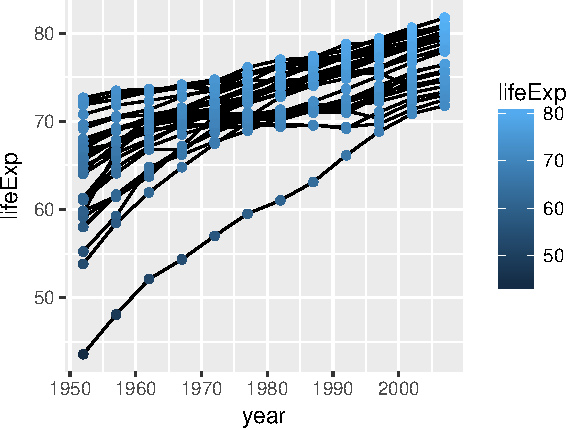
\includegraphics{04_plotting_files/figure-latex/unnamed-chunk-16-1.pdf}

\section{Extra: Optional exercises}\label{extra-optional-exercises}

\subsection{Exercise}\label{exercise-27}

Make this:

\begin{Shaded}
\begin{Highlighting}[]
\NormalTok{mydata}\OperatorTok{$}\NormalTok{dummy =}\StringTok{ }\DecValTok{1}  \CommentTok{# create a column called "dummy" that includes number 1 for each country}

\NormalTok{mydata2007 =}\StringTok{ }\NormalTok{mydata }\OperatorTok\StringTok{ }
\StringTok{  }\KeywordTok{filter}\NormalTok{(year}\OperatorTok{==}\KeywordTok{max}\NormalTok{(year)) }\OperatorTok\StringTok{ }
\StringTok{  }\KeywordTok{group_by}\NormalTok{(continent) }\OperatorTok\StringTok{ }
\StringTok{  }\KeywordTok{mutate}\NormalTok{(}\DataTypeTok{country_number =} \KeywordTok{cumsum}\NormalTok{(dummy))  }\CommentTok{# create a column called "country_number" that}
  \CommentTok{#is a cumulative sum of the number of countries before it - basically indexing}


\NormalTok{mydata2007 }\OperatorTok\StringTok{ }
\StringTok{  }\KeywordTok{ggplot}\NormalTok{(}\KeywordTok{aes}\NormalTok{(}\DataTypeTok{x =}\NormalTok{ continent)) }\OperatorTok{+}
\StringTok{  }\KeywordTok{geom_bar}\NormalTok{(}\KeywordTok{aes}\NormalTok{(}\DataTypeTok{colour=}\NormalTok{continent), }\DataTypeTok{fill =} \OtherTok{NA}\NormalTok{) }\OperatorTok{+}
\StringTok{  }\KeywordTok{geom_text}\NormalTok{(}\KeywordTok{aes}\NormalTok{(}\DataTypeTok{y =}\NormalTok{ country_number, }\DataTypeTok{label=}\NormalTok{country), }\DataTypeTok{size=}\DecValTok{4}\NormalTok{, }\DataTypeTok{vjust=}\DecValTok{1}\NormalTok{, }\DataTypeTok{colour=}\StringTok{'black'}\NormalTok{)}\OperatorTok{+}
\StringTok{  }\KeywordTok{theme_void}\NormalTok{()}
\end{Highlighting}
\end{Shaded}

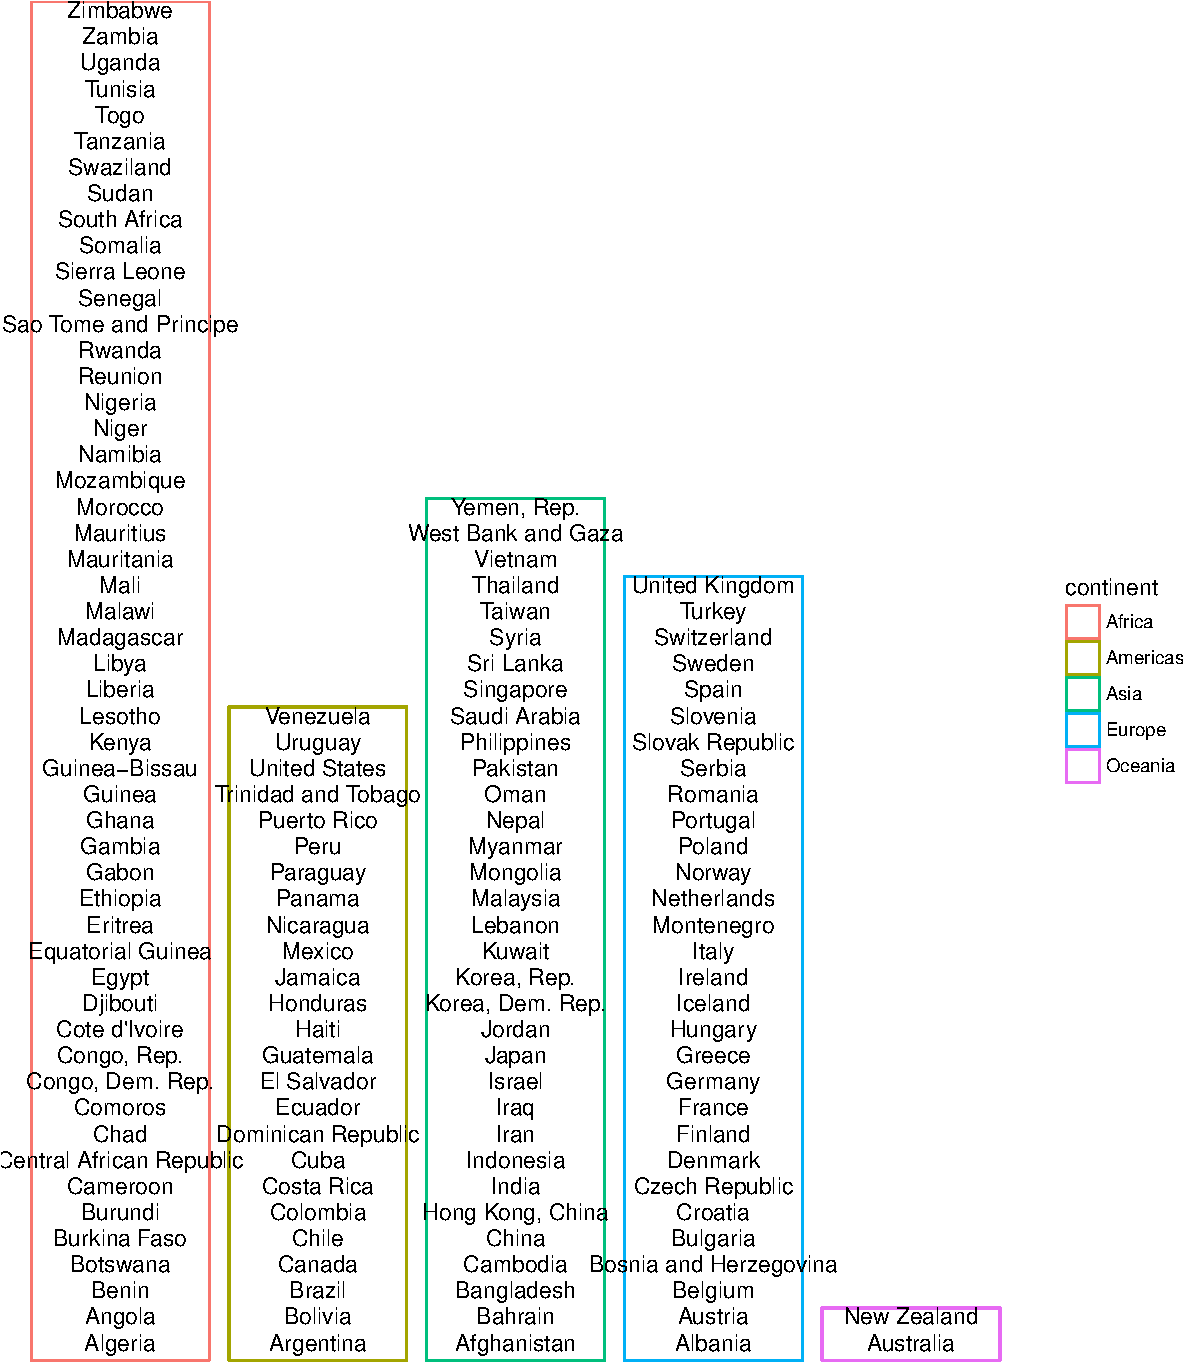
\includegraphics{04_plotting_files/figure-latex/unnamed-chunk-17-1.pdf}

\newpage

\subsection{Exercise}\label{exercise-28}

Make this:

Hints: \texttt{coord\_flip()}, \texttt{scale\_color\_gradient(...)},
\texttt{geom\_segment(...)}, \texttt{annotate("text",\ ...)}

\begin{Shaded}
\begin{Highlighting}[]
\NormalTok{mydata }\OperatorTok\StringTok{ }
\StringTok{  }\KeywordTok{filter}\NormalTok{(continent }\OperatorTok{==}\StringTok{ "Europe"}\NormalTok{) }\OperatorTok\StringTok{ }
\StringTok{  }\KeywordTok{ggplot}\NormalTok{(}\KeywordTok{aes}\NormalTok{(}\DataTypeTok{y =} \KeywordTok{fct_reorder}\NormalTok{(country, gdpPercap, }\DataTypeTok{fun=}\NormalTok{max), }\DataTypeTok{x=}\NormalTok{lifeExp, }\DataTypeTok{colour=}\NormalTok{year)) }\OperatorTok{+}
\StringTok{  }\KeywordTok{geom_point}\NormalTok{(}\DataTypeTok{shape =} \DecValTok{15}\NormalTok{, }\DataTypeTok{size =} \DecValTok{2}\NormalTok{) }\OperatorTok{+}
\StringTok{  }\KeywordTok{theme_bw}\NormalTok{() }\OperatorTok{+}
\StringTok{  }\KeywordTok{scale_colour_distiller}\NormalTok{(}\DataTypeTok{palette =} \StringTok{"Greens"}\NormalTok{, }\DataTypeTok{direction =} \DecValTok{1}\NormalTok{) }\OperatorTok{+}
\StringTok{  }\KeywordTok{geom_segment}\NormalTok{(}\KeywordTok{aes}\NormalTok{(}\DataTypeTok{yend =} \StringTok{"Switzerland"}\NormalTok{, }\DataTypeTok{x =} \DecValTok{85}\NormalTok{, }\DataTypeTok{y =} \StringTok{"Bosnia and Herzegovina"}\NormalTok{, }\DataTypeTok{xend =} \DecValTok{85}\NormalTok{),}
               \DataTypeTok{colour =} \StringTok{"black"}\NormalTok{, }\DataTypeTok{size=}\DecValTok{1}\NormalTok{,}
               \DataTypeTok{arrow =} \KeywordTok{arrow}\NormalTok{(}\DataTypeTok{length =} \KeywordTok{unit}\NormalTok{(}\FloatTok{0.3}\NormalTok{, }\StringTok{"cm"}\NormalTok{))) }\OperatorTok{+}
\StringTok{  }\KeywordTok{annotate}\NormalTok{(}\StringTok{"text"}\NormalTok{, }\DataTypeTok{y =} \StringTok{"Greece"}\NormalTok{, }\DataTypeTok{x=}\DecValTok{83}\NormalTok{, }\DataTypeTok{label =} \StringTok{"Higher GDP per capita"}\NormalTok{, }\DataTypeTok{angle =} \DecValTok{90}\NormalTok{)}
\end{Highlighting}
\end{Shaded}

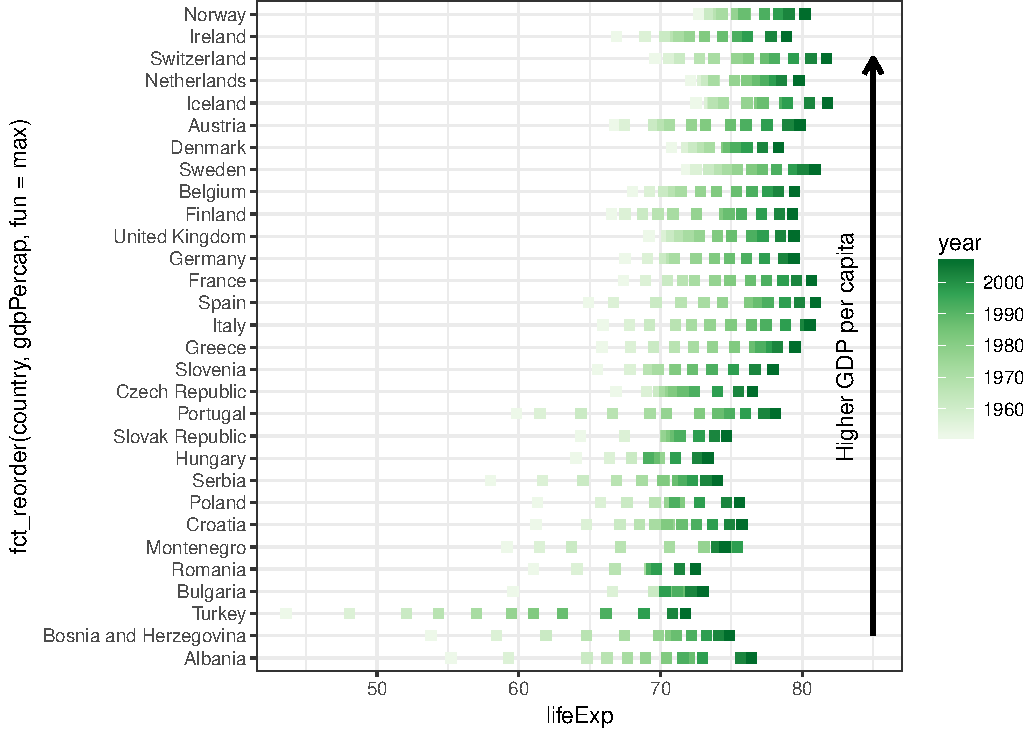
\includegraphics{04_plotting_files/figure-latex/unnamed-chunk-18-1.pdf}

\section{Solutions}\label{solutions-2}

\textbf{4.2.1}

\begin{Shaded}
\begin{Highlighting}[]
\NormalTok{mydata }\OperatorTok\StringTok{ }
\StringTok{  }\KeywordTok{filter}\NormalTok{(year }\OperatorTok{==}\StringTok{ }\DecValTok{2007}\NormalTok{) }\OperatorTok\StringTok{ }
\StringTok{  }\KeywordTok{ggplot}\NormalTok{(  }\KeywordTok{aes}\NormalTok{(}\DataTypeTok{x =}\NormalTok{ gdpPercap}\OperatorTok{/}\DecValTok{1000}\NormalTok{, }\CommentTok{#divide by 1000 to tidy the x-axis}
               \DataTypeTok{y=}\NormalTok{lifeExp,}
               \DataTypeTok{colour=}\NormalTok{continent,}
               \DataTypeTok{size=}\NormalTok{pop)) }\OperatorTok{+}
\StringTok{  }\KeywordTok{geom_point}\NormalTok{(}\DataTypeTok{shape =} \DecValTok{1}\NormalTok{) }\OperatorTok{+}
\StringTok{  }\KeywordTok{facet_wrap}\NormalTok{(}\OperatorTok{~}\NormalTok{continent) }\OperatorTok{+}
\StringTok{  }\KeywordTok{theme_bw}\NormalTok{()}
\end{Highlighting}
\end{Shaded}

\textbf{4.3.1}

\begin{Shaded}
\begin{Highlighting}[]
\NormalTok{mydata }\OperatorTok\StringTok{ }
\StringTok{  }\KeywordTok{ggplot}\NormalTok{(  }\KeywordTok{aes}\NormalTok{(}\DataTypeTok{x =}\NormalTok{ year, }\DataTypeTok{y=}\NormalTok{lifeExp, }\DataTypeTok{group =}\NormalTok{ country, }\DataTypeTok{colour=}\NormalTok{continent)) }\OperatorTok{+}
\StringTok{  }\KeywordTok{geom_line}\NormalTok{() }\OperatorTok{+}
\StringTok{  }\KeywordTok{facet_wrap}\NormalTok{(}\OperatorTok{~}\NormalTok{continent) }\OperatorTok{+}\StringTok{ }
\StringTok{  }\KeywordTok{theme_bw}\NormalTok{() }\OperatorTok{+}
\StringTok{  }\KeywordTok{scale_colour_brewer}\NormalTok{(}\DataTypeTok{palette =} \StringTok{"Paired"}\NormalTok{)}
\end{Highlighting}
\end{Shaded}

\textbf{which}

Add
\texttt{+\ \ geom\_line(data\ =\ filter(mydata,\ country\ ==\ "France"),\ colour\ =\ "blue")}

\textbf{4.4.1}

\begin{Shaded}
\begin{Highlighting}[]
\NormalTok{mydata }\OperatorTok\StringTok{ }
\StringTok{  }\KeywordTok{filter}\NormalTok{(year }\OperatorTok{==}\StringTok{ }\DecValTok{2007}\NormalTok{) }\OperatorTok\StringTok{ }
\StringTok{  }\KeywordTok{ggplot}\NormalTok{(}\KeywordTok{aes}\NormalTok{(}\DataTypeTok{x =}\NormalTok{ continent, }\DataTypeTok{y =}\NormalTok{ lifeExp)) }\OperatorTok{+}
\StringTok{  }\KeywordTok{geom_boxplot}\NormalTok{(}\DataTypeTok{outlier.shape =} \OtherTok{NA}\NormalTok{) }\OperatorTok{+}
\StringTok{  }\KeywordTok{geom_jitter}\NormalTok{(}\KeywordTok{aes}\NormalTok{(}\DataTypeTok{colour=}\NormalTok{continent), }\DataTypeTok{width=}\FloatTok{0.3}\NormalTok{, }\DataTypeTok{alpha=}\FloatTok{0.8}\NormalTok{) }\OperatorTok{+}\StringTok{ }\CommentTok{#width defaults to 0.8 of box width}
\StringTok{  }\KeywordTok{theme_bw}\NormalTok{()}
\end{Highlighting}
\end{Shaded}

\begin{Shaded}
\begin{Highlighting}[]
\NormalTok{mydata }\OperatorTok\StringTok{ }
\StringTok{  }\KeywordTok{filter}\NormalTok{(year }\OperatorTok{==}\StringTok{ }\DecValTok{2007}\NormalTok{) }\OperatorTok\StringTok{ }
\StringTok{  }\KeywordTok{ggplot}\NormalTok{(}\KeywordTok{aes}\NormalTok{(}\DataTypeTok{x =}\NormalTok{ continent, }\DataTypeTok{y =}\NormalTok{ lifeExp)) }\OperatorTok{+}
\StringTok{  }\KeywordTok{geom_boxplot}\NormalTok{(}\DataTypeTok{outlier.shape =} \OtherTok{NA}\NormalTok{) }\OperatorTok{+}
\StringTok{  }\KeywordTok{geom_jitter}\NormalTok{(}\KeywordTok{aes}\NormalTok{(}\DataTypeTok{colour=}\NormalTok{continent), }\DataTypeTok{width=}\FloatTok{0.3}\NormalTok{, }\DataTypeTok{alpha=}\FloatTok{0.8}\NormalTok{)}
  \KeywordTok{theme_bw}\NormalTok{()}
\end{Highlighting}
\end{Shaded}

\textbf{4.5.1}

\begin{Shaded}
\begin{Highlighting}[]
\NormalTok{mydata }\OperatorTok\StringTok{ }
\StringTok{  }\KeywordTok{filter}\NormalTok{(year }\OperatorTok{==}\StringTok{ }\DecValTok{2007}\NormalTok{) }\OperatorTok
\StringTok{  }\KeywordTok{filter}\NormalTok{(continent }\OperatorTok{==}\StringTok{ "Europe"}\NormalTok{) }\OperatorTok\StringTok{ }
\StringTok{  }\KeywordTok{ggplot}\NormalTok{(}\KeywordTok{aes}\NormalTok{(}\DataTypeTok{x =}\NormalTok{ country, }\DataTypeTok{y =}\NormalTok{ lifeExp)) }\OperatorTok{+}
\StringTok{  }\KeywordTok{geom_col}\NormalTok{(}\DataTypeTok{colour =} \StringTok{"#91bfdb"}\NormalTok{, }\DataTypeTok{fill =} \OtherTok{NA}\NormalTok{) }\OperatorTok{+}
\StringTok{  }\KeywordTok{coord_flip}\NormalTok{() }\OperatorTok{+}
\StringTok{  }\KeywordTok{theme_classic}\NormalTok{()}
\end{Highlighting}
\end{Shaded}

\chapter{Fine tuning plots}\label{fine-tuning-plots}

\section{Data and initial plot}\label{data-and-initial-plot}

We can save a \texttt{ggplot()} object into a variable (usually called
\texttt{p} but can be any name). This then appear in the Environment
tab. To plot it it needs to be recalled on a separate line. Saving a
plot into a variable allows us to modify it later (e.g.,
\texttt{p+theme\_bw()}).

\begin{Shaded}
\begin{Highlighting}[]
\KeywordTok{library}\NormalTok{(gapminder)}
\KeywordTok{library}\NormalTok{(tidyverse)}

\NormalTok{mydata =}\StringTok{ }\NormalTok{gapminder}

\NormalTok{mydata}\OperatorTok{$}\NormalTok{year }\OperatorTok\StringTok{ }\KeywordTok{unique}\NormalTok{()}
\end{Highlighting}
\end{Shaded}

\begin{verbatim}
##  [1] 1952 1957 1962 1967 1972 1977 1982 1987 1992 1997 2002 2007
\end{verbatim}

\begin{Shaded}
\begin{Highlighting}[]
\NormalTok{p =}\StringTok{ }\NormalTok{gapminder }\OperatorTok\StringTok{ }
\StringTok{  }\KeywordTok{filter}\NormalTok{(year }\OperatorTok{==}\StringTok{ }\DecValTok{2007}\NormalTok{) }\OperatorTok\StringTok{ }
\StringTok{  }\KeywordTok{group_by}\NormalTok{(continent, year) }\OperatorTok\StringTok{ }
\StringTok{  }\KeywordTok{ggplot}\NormalTok{(}\KeywordTok{aes}\NormalTok{(}\DataTypeTok{y =}\NormalTok{ lifeExp, }\DataTypeTok{x =}\NormalTok{ gdpPercap, }\DataTypeTok{colour =}\NormalTok{ continent)) }\OperatorTok{+}
\StringTok{  }\KeywordTok{geom_point}\NormalTok{(}\DataTypeTok{alpha =} \FloatTok{0.3}\NormalTok{) }\OperatorTok{+}
\StringTok{  }\KeywordTok{theme_bw}\NormalTok{() }\OperatorTok{+}
\StringTok{  }\KeywordTok{geom_smooth}\NormalTok{(}\DataTypeTok{method =} \StringTok{"lm"}\NormalTok{, }\DataTypeTok{se =} \OtherTok{FALSE}\NormalTok{) }\OperatorTok{+}
\StringTok{  }\KeywordTok{scale_colour_brewer}\NormalTok{(}\DataTypeTok{palette =} \StringTok{"Set1"}\NormalTok{)}

\NormalTok{p}
\end{Highlighting}
\end{Shaded}

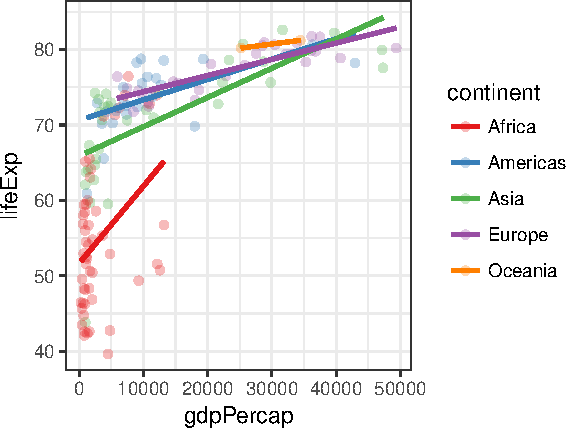
\includegraphics{05_fine_tuning_plots_files/figure-latex/unnamed-chunk-1-1.pdf}

\section{Scales}\label{scales}

\subsection{Logarithmic}\label{logarithmic}

\begin{Shaded}
\begin{Highlighting}[]
\NormalTok{p }\OperatorTok{+}\StringTok{ }\KeywordTok{scale_x_log10}\NormalTok{()}
\end{Highlighting}
\end{Shaded}

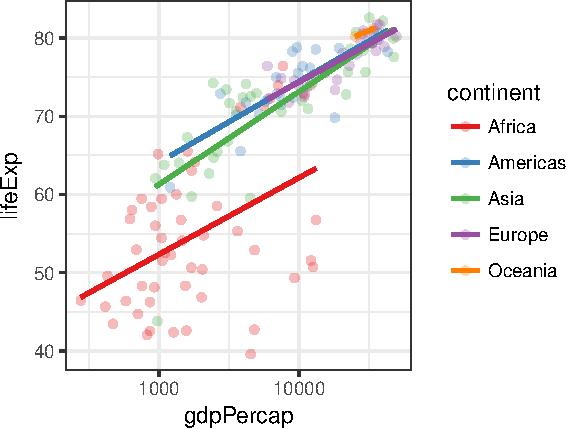
\includegraphics{05_fine_tuning_plots_files/figure-latex/unnamed-chunk-2-1.pdf}

\subsection{Expand limits}\label{expand-limits}

Specify the value you want to be included:

\begin{Shaded}
\begin{Highlighting}[]
\NormalTok{p }\OperatorTok{+}\StringTok{ }\KeywordTok{expand_limits}\NormalTok{(}\DataTypeTok{y =} \DecValTok{0}\NormalTok{)}
\end{Highlighting}
\end{Shaded}

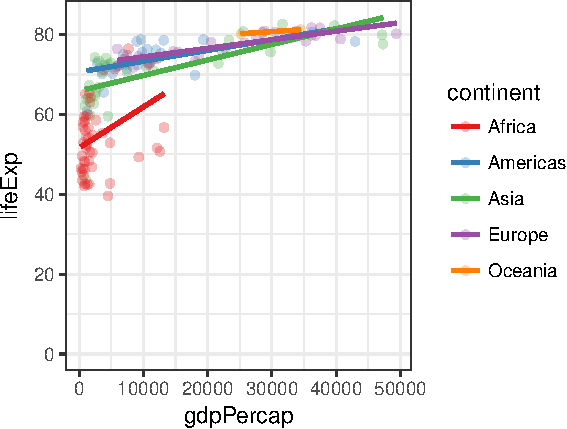
\includegraphics{05_fine_tuning_plots_files/figure-latex/unnamed-chunk-3-1.pdf}

\newpage 

Or two:

\begin{Shaded}
\begin{Highlighting}[]
\NormalTok{p }\OperatorTok{+}\StringTok{ }\KeywordTok{expand_limits}\NormalTok{(}\DataTypeTok{y =} \KeywordTok{c}\NormalTok{(}\DecValTok{0}\NormalTok{, }\DecValTok{100}\NormalTok{))}
\end{Highlighting}
\end{Shaded}

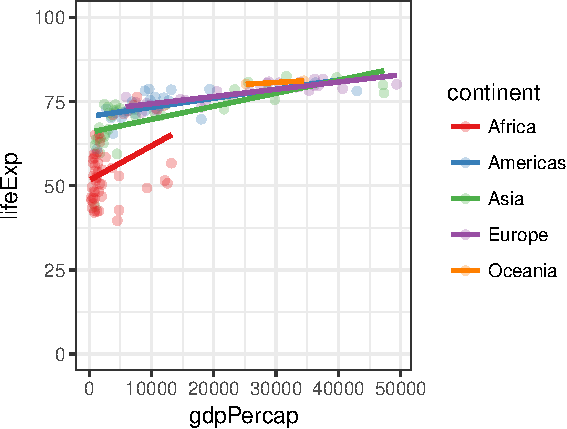
\includegraphics{05_fine_tuning_plots_files/figure-latex/unnamed-chunk-4-1.pdf}

By default, \texttt{ggplot} adds some padding around the included area
(see how the scale doesn't start from 0, but slightly before). You can
remove this padding with the expand option:

\begin{Shaded}
\begin{Highlighting}[]
\NormalTok{p }\OperatorTok{+}
\StringTok{  }\KeywordTok{expand_limits}\NormalTok{(}\DataTypeTok{y =} \KeywordTok{c}\NormalTok{(}\DecValTok{0}\NormalTok{, }\DecValTok{100}\NormalTok{)) }\OperatorTok{+}
\StringTok{  }\KeywordTok{coord_cartesian}\NormalTok{(}\DataTypeTok{expand =} \OtherTok{FALSE}\NormalTok{)}
\end{Highlighting}
\end{Shaded}

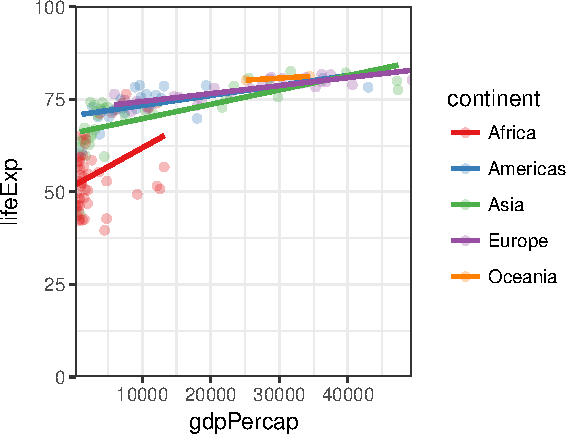
\includegraphics{05_fine_tuning_plots_files/figure-latex/unnamed-chunk-5-1.pdf}

\subsection{Zoom in}\label{zoom-in}

\begin{Shaded}
\begin{Highlighting}[]
\NormalTok{p }\OperatorTok{+}\StringTok{ }\KeywordTok{coord_cartesian}\NormalTok{(}\DataTypeTok{ylim =} \KeywordTok{c}\NormalTok{(}\DecValTok{70}\NormalTok{, }\DecValTok{85}\NormalTok{), }\DataTypeTok{xlim =} \KeywordTok{c}\NormalTok{(}\DecValTok{20000}\NormalTok{, }\DecValTok{40000}\NormalTok{))}
\end{Highlighting}
\end{Shaded}

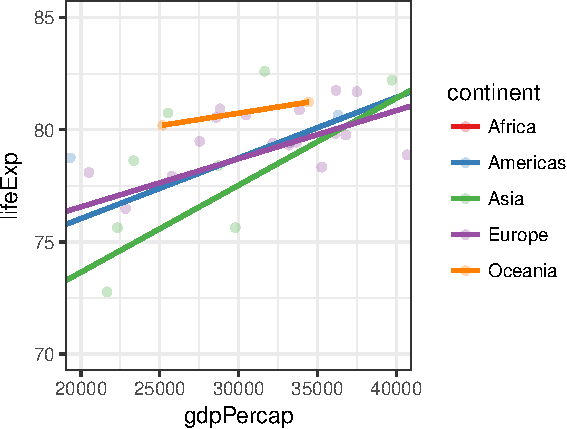
\includegraphics{05_fine_tuning_plots_files/figure-latex/unnamed-chunk-6-1.pdf}

\subsection{Exercise}\label{exercise-29}

How is this one different to the previous:

\begin{Shaded}
\begin{Highlighting}[]
\NormalTok{p }\OperatorTok{+}
\StringTok{  }\KeywordTok{scale_y_continuous}\NormalTok{(}\DataTypeTok{limits =} \KeywordTok{c}\NormalTok{(}\DecValTok{70}\NormalTok{, }\DecValTok{85}\NormalTok{)) }\OperatorTok{+}
\StringTok{  }\KeywordTok{scale_x_continuous}\NormalTok{(}\DataTypeTok{limits =} \KeywordTok{c}\NormalTok{(}\DecValTok{20000}\NormalTok{, }\DecValTok{40000}\NormalTok{))}
\end{Highlighting}
\end{Shaded}

\begin{verbatim}
## Warning: Removed 114 rows containing non-finite values (stat_smooth).
\end{verbatim}

\begin{verbatim}
## Warning: Removed 114 rows containing missing values (geom_point).
\end{verbatim}

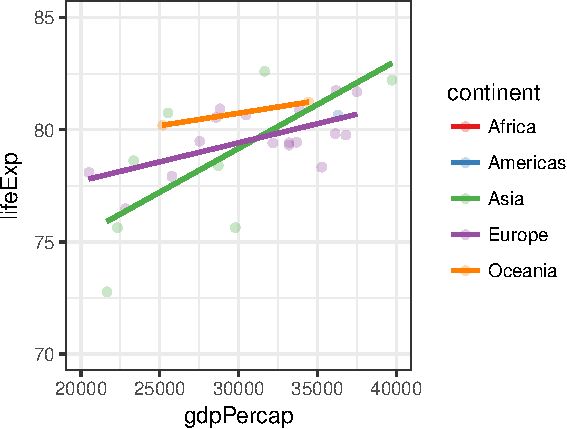
\includegraphics{05_fine_tuning_plots_files/figure-latex/unnamed-chunk-7-1.pdf}

Answer: the first one zooms in, still retaining information about the
excluded points when calculating the linear regression lines. The second
one removes the data (as the warnings say), calculating the linear
regression lines only for the visible points.

\subsection{Axis ticks}\label{axis-ticks}

\begin{Shaded}
\begin{Highlighting}[]
\NormalTok{p }\OperatorTok{+}
\StringTok{  }\KeywordTok{coord_cartesian}\NormalTok{(}\DataTypeTok{ylim =} \KeywordTok{c}\NormalTok{(}\DecValTok{0}\NormalTok{, }\DecValTok{100}\NormalTok{), }\DataTypeTok{expand =} \DecValTok{0}\NormalTok{) }\OperatorTok{+}
\StringTok{  }\KeywordTok{scale_y_continuous}\NormalTok{(}\DataTypeTok{breaks =} \KeywordTok{c}\NormalTok{(}\DecValTok{17}\NormalTok{, }\DecValTok{35}\NormalTok{, }\DecValTok{88}\NormalTok{))}
\end{Highlighting}
\end{Shaded}

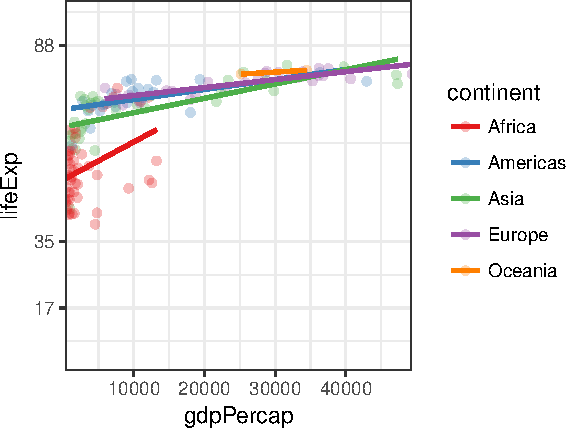
\includegraphics{05_fine_tuning_plots_files/figure-latex/unnamed-chunk-8-1.pdf}

\subsection{Swap the axes}\label{swap-the-axes}

\begin{Shaded}
\begin{Highlighting}[]
\NormalTok{p }\OperatorTok{+}
\StringTok{  }\KeywordTok{coord_flip}\NormalTok{()}
\end{Highlighting}
\end{Shaded}

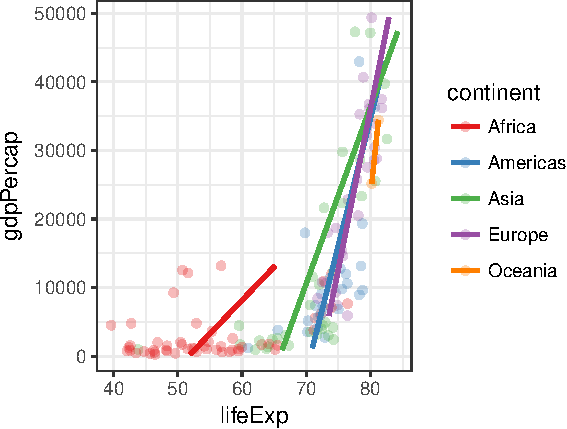
\includegraphics{05_fine_tuning_plots_files/figure-latex/unnamed-chunk-9-1.pdf}

\section{Colours}\label{colours}

\subsection{Using the Brewer palettes:}\label{using-the-brewer-palettes}

\begin{Shaded}
\begin{Highlighting}[]
\NormalTok{p }\OperatorTok{+}
\StringTok{  }\KeywordTok{scale_color_brewer}\NormalTok{(}\DataTypeTok{palette =} \StringTok{"Paired"}\NormalTok{)}
\end{Highlighting}
\end{Shaded}

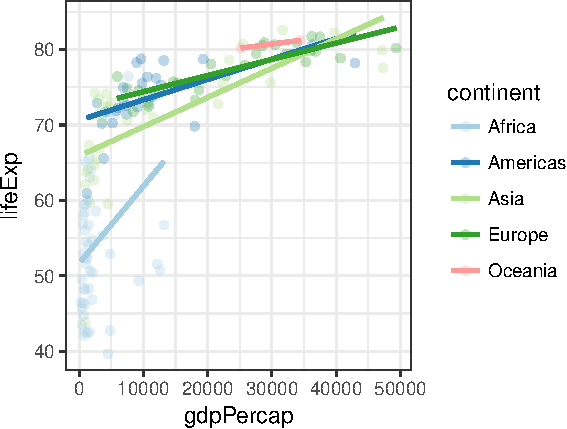
\includegraphics{05_fine_tuning_plots_files/figure-latex/unnamed-chunk-10-1.pdf}

\subsection{Legend title}\label{legend-title}

\texttt{scale\_colour\_brewer()} is also a conventient place to change
the legend title:

\begin{Shaded}
\begin{Highlighting}[]
\NormalTok{p }\OperatorTok{+}
\StringTok{  }\KeywordTok{scale_color_brewer}\NormalTok{(}\StringTok{"Continent - }\CharTok{\textbackslash{}n}\StringTok{ one of 5"}\NormalTok{, }\DataTypeTok{palette =} \StringTok{"Paired"}\NormalTok{)}
\end{Highlighting}
\end{Shaded}

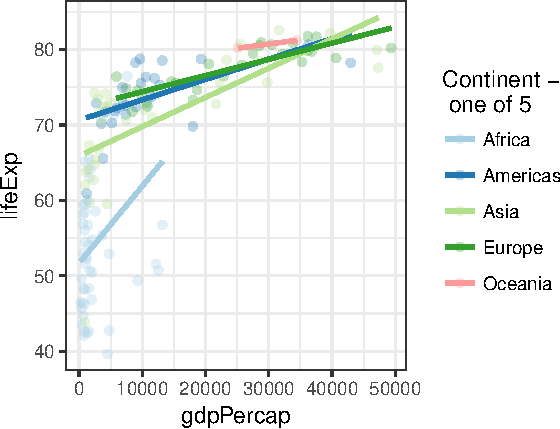
\includegraphics{05_fine_tuning_plots_files/figure-latex/unnamed-chunk-11-1.pdf}

Note the \texttt{\textbackslash{}n} inside the new legend title - new
line.

\subsection{Choosing colours manually}\label{choosing-colours-manually}

Use words:

\begin{Shaded}
\begin{Highlighting}[]
\NormalTok{p }\OperatorTok{+}
\StringTok{  }\KeywordTok{scale_color_manual}\NormalTok{(}\DataTypeTok{values =} \KeywordTok{c}\NormalTok{(}\StringTok{"red"}\NormalTok{, }\StringTok{"green"}\NormalTok{, }\StringTok{"blue"}\NormalTok{, }\StringTok{"purple"}\NormalTok{, }\StringTok{"pink"}\NormalTok{))}
\end{Highlighting}
\end{Shaded}

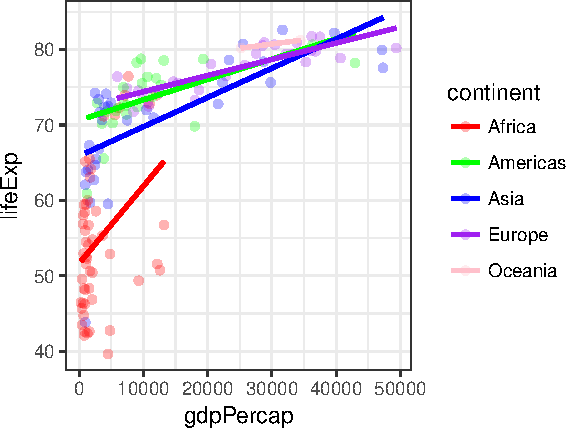
\includegraphics{05_fine_tuning_plots_files/figure-latex/unnamed-chunk-12-1.pdf}

Or HEX codes (either from \url{http://colorbrewer2.org/} or any other
resource):

\begin{Shaded}
\begin{Highlighting}[]
\NormalTok{p }\OperatorTok{+}
\StringTok{  }\KeywordTok{scale_color_manual}\NormalTok{(}\DataTypeTok{values =} \KeywordTok{c}\NormalTok{(}\StringTok{"#e41a1c"}\NormalTok{, }\StringTok{"#377eb8"}\NormalTok{, }\StringTok{"#4daf4a"}\NormalTok{, }\StringTok{"#984ea3"}\NormalTok{, }\StringTok{"#ff7f00"}\NormalTok{))}
\end{Highlighting}
\end{Shaded}

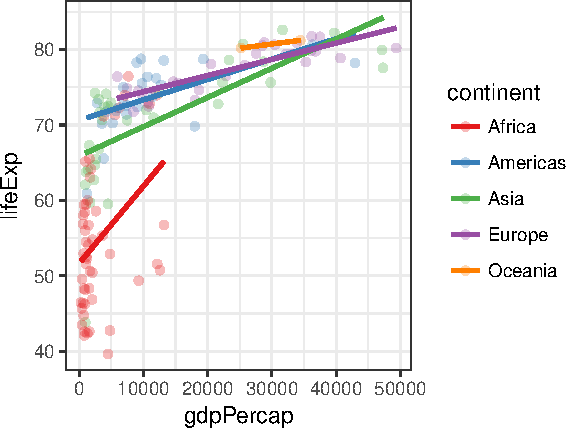
\includegraphics{05_fine_tuning_plots_files/figure-latex/unnamed-chunk-13-1.pdf}

Note that \url{http://colorbrewer2.org/} also has options for
\emph{Colourblind safe} and \emph{Print friendly}.

\newpage 

\section{Titles and labels}\label{titles-and-labels}

\begin{Shaded}
\begin{Highlighting}[]
\NormalTok{p }\OperatorTok{+}
\StringTok{  }\KeywordTok{labs}\NormalTok{(}\DataTypeTok{x =} \StringTok{"Gross domestic product per capita"}\NormalTok{,}
         \DataTypeTok{y =} \StringTok{"Life expectancy"}\NormalTok{,}
         \DataTypeTok{title =} \StringTok{"Health and economics"}\NormalTok{,}
         \DataTypeTok{subtitle =} \StringTok{"Gapminder dataset, 2007"}\NormalTok{)}
\end{Highlighting}
\end{Shaded}

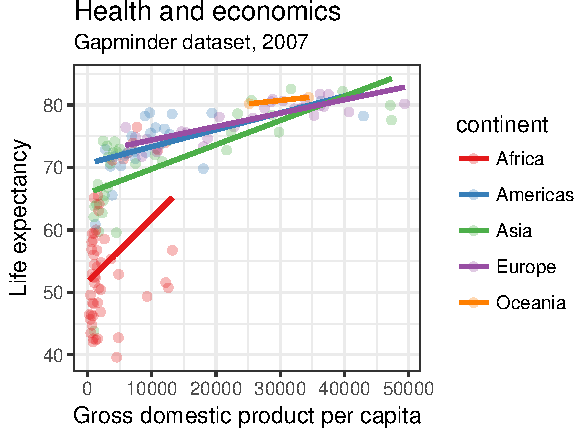
\includegraphics{05_fine_tuning_plots_files/figure-latex/unnamed-chunk-14-1.pdf}

\subsection{Annotation}\label{annotation}

\begin{Shaded}
\begin{Highlighting}[]
\NormalTok{p }\OperatorTok{+}
\StringTok{  }\KeywordTok{annotate}\NormalTok{(}\StringTok{"text"}\NormalTok{,}
           \DataTypeTok{x =} \DecValTok{25000}\NormalTok{,}
           \DataTypeTok{y =} \DecValTok{50}\NormalTok{,}
           \DataTypeTok{label =} \StringTok{"No points here!"}\NormalTok{)}
\end{Highlighting}
\end{Shaded}

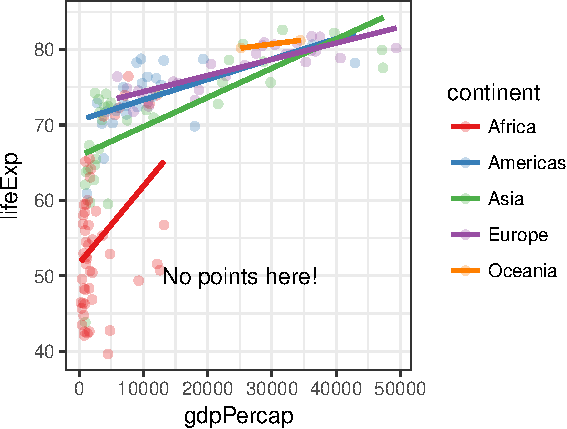
\includegraphics{05_fine_tuning_plots_files/figure-latex/unnamed-chunk-15-1.pdf}

\begin{Shaded}
\begin{Highlighting}[]
\NormalTok{p }\OperatorTok{+}
\StringTok{  }\KeywordTok{annotate}\NormalTok{(}\StringTok{"label"}\NormalTok{,}
           \DataTypeTok{x =} \DecValTok{25000}\NormalTok{,}
           \DataTypeTok{y =} \DecValTok{50}\NormalTok{,}
           \DataTypeTok{label =} \StringTok{"No points here!"}\NormalTok{)}
\end{Highlighting}
\end{Shaded}

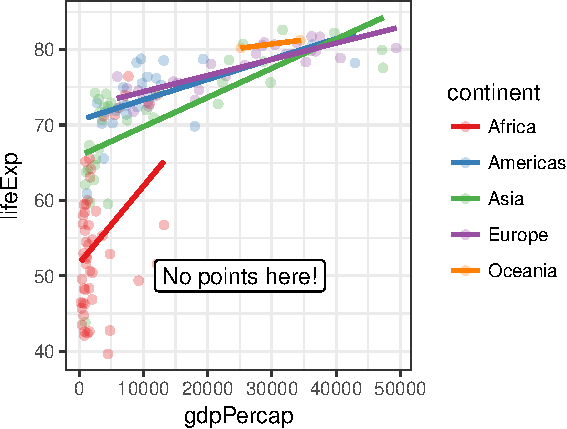
\includegraphics{05_fine_tuning_plots_files/figure-latex/unnamed-chunk-16-1.pdf}

\begin{Shaded}
\begin{Highlighting}[]
\NormalTok{p }\OperatorTok{+}
\StringTok{  }\KeywordTok{annotate}\NormalTok{(}\StringTok{"label"}\NormalTok{,}
           \DataTypeTok{x =} \DecValTok{25000}\NormalTok{, }
           \DataTypeTok{y =} \DecValTok{50}\NormalTok{,}
           \DataTypeTok{label =} \StringTok{"No points here!"}\NormalTok{, }
           \DataTypeTok{hjust =} \DecValTok{0}\NormalTok{)}
\end{Highlighting}
\end{Shaded}

\includegraphics{05_fine_tuning_plots_files/figure-latex/unnamed-chunk-17-1.pdf}

\texttt{hjust} stand for horizontal justification. It's default value is
0.5 (see how the label was centered at 25,000 - our chosen x location),
0 means the label goes to the right from 25,000, 1 would make it end at
25,000.

\subsection{Annotation with a superscript and a
variable}\label{annotation-with-a-superscript-and-a-variable}

\begin{Shaded}
\begin{Highlighting}[]
\NormalTok{fit_glance =}\StringTok{ }\KeywordTok{data.frame}\NormalTok{(}\DataTypeTok{r.squared =} \FloatTok{0.7693465}\NormalTok{)}


\NormalTok{plot_rsquared =}\StringTok{ }\KeywordTok{paste0}\NormalTok{(}
  \StringTok{"R^2 == "}\NormalTok{,}
\NormalTok{  fit_glance}\OperatorTok{$}\NormalTok{r.squared }\OperatorTok\StringTok{ }\KeywordTok{round}\NormalTok{(}\DecValTok{2}\NormalTok{))}


\NormalTok{p }\OperatorTok{+}
\StringTok{  }\KeywordTok{annotate}\NormalTok{(}\StringTok{"text"}\NormalTok{,}
           \DataTypeTok{x =} \DecValTok{25000}\NormalTok{, }
           \DataTypeTok{y =} \DecValTok{50}\NormalTok{,}
           \DataTypeTok{label =}\NormalTok{ plot_rsquared, }\DataTypeTok{parse =} \OtherTok{TRUE}\NormalTok{,}
           \DataTypeTok{hjust =} \DecValTok{0}\NormalTok{)}
\end{Highlighting}
\end{Shaded}

\includegraphics{05_fine_tuning_plots_files/figure-latex/unnamed-chunk-18-1.pdf}

\section{Text size}\label{text-size}

\begin{Shaded}
\begin{Highlighting}[]
\NormalTok{p }\OperatorTok{+}
\StringTok{  }\KeywordTok{theme}\NormalTok{(}\DataTypeTok{axis.text.y =} \KeywordTok{element_text}\NormalTok{(}\DataTypeTok{size =} \DecValTok{16}\NormalTok{),}
        \DataTypeTok{axis.text.x =} \KeywordTok{element_text}\NormalTok{(}\DataTypeTok{colour =} \StringTok{"red"}\NormalTok{, }\DataTypeTok{angle =} \DecValTok{45}\NormalTok{, }\DataTypeTok{vjust =} \FloatTok{0.5}\NormalTok{),}
        \DataTypeTok{axis.title =} \KeywordTok{element_text}\NormalTok{(}\DataTypeTok{size =} \DecValTok{16}\NormalTok{, }\DataTypeTok{colour =} \StringTok{"darkgreen"}\NormalTok{)}
\NormalTok{        )}
\end{Highlighting}
\end{Shaded}

\includegraphics{05_fine_tuning_plots_files/figure-latex/unnamed-chunk-19-1.pdf}

\subsection{Legend position}\label{legend-position}

Use the following words: \texttt{"right",\ "left",\ "top",\ "bottom"},
or ``none'' to remove the legend.

\begin{Shaded}
\begin{Highlighting}[]
\NormalTok{p }\OperatorTok{+}
\StringTok{  }\KeywordTok{theme}\NormalTok{(}\DataTypeTok{legend.position =} \StringTok{"none"}\NormalTok{)}
\end{Highlighting}
\end{Shaded}

\includegraphics{05_fine_tuning_plots_files/figure-latex/unnamed-chunk-20-1.pdf}

Or use relative coordinates (0--1) to give it an -y location:

\begin{Shaded}
\begin{Highlighting}[]
\NormalTok{p }\OperatorTok{+}
\StringTok{  }\KeywordTok{theme}\NormalTok{(}\DataTypeTok{legend.position=}\KeywordTok{c}\NormalTok{(}\DecValTok{1}\NormalTok{,}\DecValTok{0}\NormalTok{),}
        \DataTypeTok{legend.justification=}\KeywordTok{c}\NormalTok{(}\DecValTok{1}\NormalTok{,}\DecValTok{0}\NormalTok{)) }\CommentTok{#bottom-right corner}
\end{Highlighting}
\end{Shaded}

\includegraphics{05_fine_tuning_plots_files/figure-latex/unnamed-chunk-21-1.pdf}

\begin{Shaded}
\begin{Highlighting}[]
\NormalTok{p }\OperatorTok{+}
\StringTok{  }\KeywordTok{theme}\NormalTok{(}\DataTypeTok{legend.position =} \StringTok{"top"}\NormalTok{) }\OperatorTok{+}
\StringTok{  }\KeywordTok{guides}\NormalTok{(}\DataTypeTok{colour =} \KeywordTok{guide_legend}\NormalTok{(}\DataTypeTok{ncol=}\DecValTok{2}\NormalTok{))}
\end{Highlighting}
\end{Shaded}

\includegraphics{05_fine_tuning_plots_files/figure-latex/unnamed-chunk-22-1.pdf}

\section{Saving your plot}\label{saving-your-plot}

\begin{Shaded}
\begin{Highlighting}[]
\KeywordTok{ggsave}\NormalTok{(p, }\DataTypeTok{file =} \StringTok{"my_saved_plot.png"}\NormalTok{, }\DataTypeTok{width =} \DecValTok{5}\NormalTok{, }\DataTypeTok{height =} \DecValTok{4}\NormalTok{)}
\end{Highlighting}
\end{Shaded}

\chapter*{(PART *) Part II: Medical
Statistics}\label{part-part-ii-medical-statistics}
\addcontentsline{toc}{chapter}{(PART *) Part II: Medical Statistics}

\chapter{Tests for continuous outcome
variables}\label{tests-for-continuous-outcome-variables}

\section{Load data}\label{load-data}

This session we will be using the gapminder dataset as in Session 4.

\begin{Shaded}
\begin{Highlighting}[]
\KeywordTok{library}\NormalTok{(tidyverse) }
\KeywordTok{library}\NormalTok{(gapminder)}
\KeywordTok{library}\NormalTok{(broom)}

\NormalTok{mydata =}\StringTok{ }\NormalTok{gapminder}
\end{Highlighting}
\end{Shaded}

The first step of choosing the right statistical test is determining the
type of variable you have.

Lets first have a look at some of our avalible data:

\begin{Shaded}
\begin{Highlighting}[]
\NormalTok{mydata}\OperatorTok{$}\NormalTok{continent }\OperatorTok\StringTok{ }\KeywordTok{unique}\NormalTok{() }\CommentTok{# categorical}
\end{Highlighting}
\end{Shaded}

\begin{verbatim}
## [1] Asia     Europe   Africa   Americas Oceania 
## Levels: Africa Americas Asia Europe Oceania
\end{verbatim}

\begin{Shaded}
\begin{Highlighting}[]
\NormalTok{mydata}\OperatorTok{$}\NormalTok{year }\OperatorTok\StringTok{ }\KeywordTok{unique}\NormalTok{() }\CommentTok{# categorical}
\end{Highlighting}
\end{Shaded}

\begin{verbatim}
##  [1] 1952 1957 1962 1967 1972 1977 1982 1987 1992 1997 2002 2007
\end{verbatim}

\begin{Shaded}
\begin{Highlighting}[]
\NormalTok{mydata}\OperatorTok{$}\NormalTok{lifeExp }\OperatorTok\StringTok{ }\KeywordTok{head}\NormalTok{() }\CommentTok{# continuous}
\end{Highlighting}
\end{Shaded}

\begin{verbatim}
## [1] 28.801 30.332 31.997 34.020 36.088 38.438
\end{verbatim}

\section{T-test}\label{t-test}

A t-test is used to compare the means of two groups of continuous
variables.

\subsection{Plotting}\label{plotting}

Before you perform any statistical tests, you should always plot your
data first to determine whether these have a ``normal'' distribution.

\begin{itemize}
\item
  Histograms should form a symmetrical ``bell-shaped curve''.
\item
  Q-Q plots should fall along the 45 degree line.
\item
  Box-plots should be symmetrical and have few outliers.
\end{itemize}

\subsection{Histogram for each
continent}\label{histogram-for-each-continent}

\begin{Shaded}
\begin{Highlighting}[]
\KeywordTok{theme_set}\NormalTok{(}\KeywordTok{theme_bw}\NormalTok{())}

\NormalTok{mydata }\OperatorTok\StringTok{ }
\StringTok{    }\KeywordTok{filter}\NormalTok{(year }\OperatorTok\StringTok{ }\KeywordTok{c}\NormalTok{(}\DecValTok{2002}\NormalTok{, }\DecValTok{2007}\NormalTok{)) }\OperatorTok
\StringTok{    }\KeywordTok{ggplot}\NormalTok{(}\KeywordTok{aes}\NormalTok{(}\DataTypeTok{x =}\NormalTok{ lifeExp)) }\OperatorTok{+}
\StringTok{    }\KeywordTok{geom_histogram}\NormalTok{(}\DataTypeTok{bins =} \DecValTok{10}\NormalTok{) }\OperatorTok{+}
\StringTok{    }\KeywordTok{facet_grid}\NormalTok{(year}\OperatorTok{~}\NormalTok{continent, }\DataTypeTok{scales =} \StringTok{"free"}\NormalTok{)}
\end{Highlighting}
\end{Shaded}

\includegraphics{06_tests_continuous_files/figure-latex/unnamed-chunk-3-1.pdf}

\subsection{Q-Q plot for each
continent}\label{q-q-plot-for-each-continent}

With \texttt{ggplot()}, we can drawa Q-Q plot for each subgroup very
efficiently:

\begin{Shaded}
\begin{Highlighting}[]
\NormalTok{mydata }\OperatorTok\StringTok{ }
\StringTok{  }\KeywordTok{filter}\NormalTok{(year }\OperatorTok\StringTok{ }\KeywordTok{c}\NormalTok{(}\DecValTok{2002}\NormalTok{, }\DecValTok{2007}\NormalTok{)) }\OperatorTok\StringTok{ }
\StringTok{  }\KeywordTok{ggplot}\NormalTok{(}\KeywordTok{aes}\NormalTok{(}\DataTypeTok{sample =}\NormalTok{ lifeExp)) }\OperatorTok{+}\StringTok{ }
\StringTok{  }\KeywordTok{geom_point}\NormalTok{(}\DataTypeTok{stat =} \StringTok{"qq"}\NormalTok{) }\OperatorTok{+}
\StringTok{  }\KeywordTok{facet_grid}\NormalTok{(year}\OperatorTok{~}\NormalTok{continent)}
\end{Highlighting}
\end{Shaded}

\includegraphics{06_tests_continuous_files/figure-latex/unnamed-chunk-4-1.pdf}

Or we could save a subset of the data (e.g., ``Americas'' and year 2007
only) into a new variable (\texttt{subdata}) and use base R to draw a
single Q-Q plot with less code:

\begin{Shaded}
\begin{Highlighting}[]
\NormalTok{mydata }\OperatorTok\StringTok{ }
\StringTok{  }\KeywordTok{filter}\NormalTok{(year }\OperatorTok{==}\StringTok{ }\DecValTok{2007}\NormalTok{) }\OperatorTok\StringTok{ }
\StringTok{  }\KeywordTok{filter}\NormalTok{(continent }\OperatorTok{==}\StringTok{ "Americas"}\NormalTok{) ->}\StringTok{ }\NormalTok{subdata}

\KeywordTok{qqnorm}\NormalTok{(subdata}\OperatorTok{$}\NormalTok{lifeExp)}
\KeywordTok{qqline}\NormalTok{(subdata}\OperatorTok{$}\NormalTok{lifeExp)}
\end{Highlighting}
\end{Shaded}

\includegraphics{06_tests_continuous_files/figure-latex/unnamed-chunk-5-1.pdf}

\subsection{Boxplot of 2 years}\label{boxplot-of-2-years}

\begin{Shaded}
\begin{Highlighting}[]
\NormalTok{mydata }\OperatorTok\StringTok{ }
\StringTok{    }\KeywordTok{filter}\NormalTok{(year }\OperatorTok\StringTok{ }\KeywordTok{c}\NormalTok{(}\DecValTok{2002}\NormalTok{, }\DecValTok{2007}\NormalTok{)) }\OperatorTok\StringTok{ }
\StringTok{    }\KeywordTok{ggplot}\NormalTok{(}\KeywordTok{aes}\NormalTok{(}\DataTypeTok{x =} \KeywordTok{factor}\NormalTok{(year), }\DataTypeTok{y=}\NormalTok{lifeExp)) }\OperatorTok{+}\StringTok{ }\CommentTok{#show that x = year errors: }
\StringTok{    }\KeywordTok{geom_boxplot}\NormalTok{()                           }\CommentTok{#needs to be factor(year) or group=year}
\end{Highlighting}
\end{Shaded}

\includegraphics{06_tests_continuous_files/figure-latex/unnamed-chunk-6-1.pdf}

\subsection{Exercise}\label{exercise-30}

Make a histogram, Q-Q plot, and a box-plot for the life expectancy for a
continent (you choose!) but for all years - does the data appear
normally distributed?

\section{Two-sample t-tests}\label{two-sample-t-tests}

Lets perform a t-test on the ``Americas'' data as it appears normally
distributed. We are savings the results of our t.test into a variable
called t.result, but you can call it whatever you like (e.g.
\texttt{myttest}).

\begin{Shaded}
\begin{Highlighting}[]
\NormalTok{mydata }\OperatorTok\StringTok{ }
\StringTok{  }\KeywordTok{filter}\NormalTok{(year }\OperatorTok\StringTok{ }\KeywordTok{c}\NormalTok{(}\DecValTok{2002}\NormalTok{, }\DecValTok{2007}\NormalTok{)) }\OperatorTok
\StringTok{  }\KeywordTok{filter}\NormalTok{(continent }\OperatorTok{==}\StringTok{ "Americas"}\NormalTok{) ->}\StringTok{ }\NormalTok{test.data}

\KeywordTok{t.test}\NormalTok{(lifeExp}\OperatorTok{~}\NormalTok{year, }\DataTypeTok{data=}\NormalTok{test.data)}
\end{Highlighting}
\end{Shaded}

\begin{verbatim}
## 
##  Welch Two Sample t-test
## 
## data:  lifeExp by year
## t = -0.90692, df = 47.713, p-value = 0.369
## alternative hypothesis: true difference in means is not equal to 0
## 95 percent confidence interval:
##  -3.816017  1.443857
## sample estimates:
## mean in group 2002 mean in group 2007 
##           72.42204           73.60812
\end{verbatim}

\begin{Shaded}
\begin{Highlighting}[]
\NormalTok{mydata }\OperatorTok\StringTok{ }
\StringTok{  }\KeywordTok{filter}\NormalTok{(year }\OperatorTok\StringTok{ }\KeywordTok{c}\NormalTok{(}\DecValTok{2002}\NormalTok{, }\DecValTok{2007}\NormalTok{)) }\OperatorTok
\StringTok{  }\KeywordTok{filter}\NormalTok{(continent }\OperatorTok{==}\StringTok{ "Americas"}\NormalTok{) }\OperatorTok\StringTok{ }
\StringTok{  }\KeywordTok{t.test}\NormalTok{(lifeExp}\OperatorTok{~}\NormalTok{year, }\DataTypeTok{data =}\NormalTok{ .) ->}\StringTok{ }\NormalTok{t.result}

\NormalTok{t.result}
\end{Highlighting}
\end{Shaded}

\begin{verbatim}
## 
##  Welch Two Sample t-test
## 
## data:  lifeExp by year
## t = -0.90692, df = 47.713, p-value = 0.369
## alternative hypothesis: true difference in means is not equal to 0
## 95 percent confidence interval:
##  -3.816017  1.443857
## sample estimates:
## mean in group 2002 mean in group 2007 
##           72.42204           73.60812
\end{verbatim}

\subsection{T-Test output}\label{t-test-output}

However, that output isn't in a useful format, let's investigate the
output of the function \texttt{t.test()}.

\begin{Shaded}
\begin{Highlighting}[]
\KeywordTok{names}\NormalTok{(t.result)}
\end{Highlighting}
\end{Shaded}

\begin{verbatim}
## [1] "statistic"   "parameter"   "p.value"     "conf.int"    "estimate"   
## [6] "null.value"  "alternative" "method"      "data.name"
\end{verbatim}

\begin{Shaded}
\begin{Highlighting}[]
\KeywordTok{str}\NormalTok{(t.result) }\CommentTok{# or click on the blue button in the Environment tab}
\end{Highlighting}
\end{Shaded}

\begin{verbatim}
## List of 9
##  $ statistic  : Named num -0.907
##   ..- attr(*, "names")= chr "t"
##  $ parameter  : Named num 47.7
##   ..- attr(*, "names")= chr "df"
##  $ p.value    : num 0.369
##  $ conf.int   : atomic [1:2] -3.82 1.44
##   ..- attr(*, "conf.level")= num 0.95
##  $ estimate   : Named num [1:2] 72.4 73.6
##   ..- attr(*, "names")= chr [1:2] "mean in group 2002" "mean in group 2007"
##  $ null.value : Named num 0
##   ..- attr(*, "names")= chr "difference in means"
##  $ alternative: chr "two.sided"
##  $ method     : chr "Welch Two Sample t-test"
##  $ data.name  : chr "lifeExp by year"
##  - attr(*, "class")= chr "htest"
\end{verbatim}

The structure of R's \texttt{t.test()} result looks a bit overwhelming.
Fortunately, the \texttt{tidy()} function from \texttt{library(broom)}
puts it into a neat dataframe for us:

\begin{Shaded}
\begin{Highlighting}[]
\NormalTok{t.result <-}\StringTok{ }\KeywordTok{tidy}\NormalTok{(t.result) }\CommentTok{# broom package puts it all in a data frame}
\end{Highlighting}
\end{Shaded}

try clicking on it in the Environment tab now.

Thus, now we understand the output structure we can extract any result.

\begin{Shaded}
\begin{Highlighting}[]
\NormalTok{t.result}\OperatorTok{$}\NormalTok{p.value}
\end{Highlighting}
\end{Shaded}

\begin{verbatim}
## [1] 0.3690064
\end{verbatim}

\subsection{Exercise}\label{exercise-31}

\begin{enumerate}
\def\labelenumi{\arabic{enumi}.}
\item
  Select any 2 years in any continent and perform a t-test to determine
  whether the life expectancy is signficantly different. Remember to
  plot your data first.
\item
  Extract only the p-value from your \texttt{t.test()} output.
\end{enumerate}

\section{One sample t-tests}\label{one-sample-t-tests}

However, we don't always want to compare 2 groups or sometimes we don't
have the data to be able to.

Let's investigate whether the mean life expectancy in each continent
significant different to 77 years in 2007.

\begin{Shaded}
\begin{Highlighting}[]
\NormalTok{mydata }\OperatorTok\StringTok{ }
\StringTok{  }\KeywordTok{filter}\NormalTok{(year}\OperatorTok{==}\DecValTok{2007}\NormalTok{, continent}\OperatorTok{==}\StringTok{'Europe'}\NormalTok{) ->}\StringTok{ }\NormalTok{subdata}

\CommentTok{# Standard one-sample t-test}
\KeywordTok{t.test}\NormalTok{(subdata}\OperatorTok{$}\NormalTok{lifeExp, }\DataTypeTok{mu=}\DecValTok{77}\NormalTok{)}
\end{Highlighting}
\end{Shaded}

\begin{verbatim}
## 
##  One Sample t-test
## 
## data:  subdata$lifeExp
## t = 1.1922, df = 29, p-value = 0.2428
## alternative hypothesis: true mean is not equal to 77
## 95 percent confidence interval:
##  76.53592 78.76128
## sample estimates:
## mean of x 
##   77.6486
\end{verbatim}

\subsection{Exercise}\label{exercise-32}

\begin{enumerate}
\def\labelenumi{\arabic{enumi}.}
\item
  Select a different year, different continent, and different age to
  compare the mean life expectancy to.
\item
  Replace mu=77 with mu=0 (the default value). How does this affect your
  result?
\end{enumerate}

\section{ANOVA}\label{anova}

In some cases, we may also want to test more than two groups to see if
they are signficantly different.

\subsection{Plotting}\label{plotting-1}

For example, lets plot the life expectancy in 2007 accross 3 continents.

\begin{Shaded}
\begin{Highlighting}[]
\NormalTok{mydata }\OperatorTok\StringTok{ }
\StringTok{    }\KeywordTok{filter}\NormalTok{(year }\OperatorTok{==}\StringTok{ }\DecValTok{2007}\NormalTok{) }\OperatorTok\StringTok{ }
\StringTok{    }\KeywordTok{filter}\NormalTok{(continent }\OperatorTok\StringTok{ }\KeywordTok{c}\NormalTok{(}\StringTok{"Americas"}\NormalTok{, }\StringTok{"Europe"}\NormalTok{, }\StringTok{"Asia"}\NormalTok{)) }\OperatorTok\StringTok{ }
\StringTok{    }\KeywordTok{ggplot}\NormalTok{(}\KeywordTok{aes}\NormalTok{(}\DataTypeTok{x =}\NormalTok{ continent, }\DataTypeTok{y=}\NormalTok{lifeExp)) }\OperatorTok{+}
\StringTok{    }\KeywordTok{geom_boxplot}\NormalTok{()}
\end{Highlighting}
\end{Shaded}

\includegraphics{06_tests_continuous_files/figure-latex/unnamed-chunk-12-1.pdf}

\subsection{Analysis}\label{analysis}

ANOVA tests are useful for testing for the presence of signficant
differences between more than two groups or variables.

\begin{Shaded}
\begin{Highlighting}[]
\NormalTok{mydata }\OperatorTok\StringTok{ }
\StringTok{  }\KeywordTok{filter}\NormalTok{(year }\OperatorTok{==}\StringTok{ }\DecValTok{2007}\NormalTok{) }\OperatorTok\StringTok{ }
\StringTok{  }\KeywordTok{filter}\NormalTok{(continent }\OperatorTok\StringTok{ }\KeywordTok{c}\NormalTok{(}\StringTok{"Americas"}\NormalTok{, }\StringTok{"Europe"}\NormalTok{, }\StringTok{"Asia"}\NormalTok{)) ->}\StringTok{ }\NormalTok{subdata}

\NormalTok{fit =}\StringTok{ }\KeywordTok{aov}\NormalTok{(lifeExp}\OperatorTok{~}\NormalTok{continent, }\DataTypeTok{data =}\NormalTok{ subdata) }

\KeywordTok{summary}\NormalTok{(fit)}
\end{Highlighting}
\end{Shaded}

\begin{verbatim}
##             Df Sum Sq Mean Sq F value   Pr(>F)    
## continent    2  755.6   377.8   11.63 3.42e-05 ***
## Residuals   85 2760.3    32.5                     
## ---
## Signif. codes:  0 '***' 0.001 '**' 0.01 '*' 0.05 '.' 0.1 ' ' 1
\end{verbatim}

\begin{Shaded}
\begin{Highlighting}[]
\NormalTok{mydata }\OperatorTok\StringTok{ }
\StringTok{  }\KeywordTok{filter}\NormalTok{(year }\OperatorTok{==}\StringTok{ }\DecValTok{2007}\NormalTok{) }\OperatorTok\StringTok{ }
\StringTok{  }\KeywordTok{filter}\NormalTok{(continent }\OperatorTok\StringTok{ }\KeywordTok{c}\NormalTok{(}\StringTok{"Americas"}\NormalTok{, }\StringTok{"Europe"}\NormalTok{, }\StringTok{"Asia"}\NormalTok{)) }\OperatorTok\StringTok{ }
\StringTok{  }\KeywordTok{aov}\NormalTok{(lifeExp}\OperatorTok{~}\NormalTok{continent, }\DataTypeTok{data =}\NormalTok{ .) }\OperatorTok\StringTok{ }
\StringTok{    }\KeywordTok{tidy}\NormalTok{()}
\end{Highlighting}
\end{Shaded}

\begin{verbatim}
##        term df     sumsq    meansq statistic     p.value
## 1 continent  2  755.6178 377.80892  11.63417 3.41973e-05
## 2 Residuals 85 2760.2966  32.47408        NA          NA
\end{verbatim}

\subsection{Check assumptions}\label{check-assumptions}

\begin{Shaded}
\begin{Highlighting}[]
\CommentTok{# Check ANOVA assumptions }
\KeywordTok{par}\NormalTok{(}\DataTypeTok{mfrow=}\KeywordTok{c}\NormalTok{(}\DecValTok{2}\NormalTok{, }\DecValTok{2}\NormalTok{)) }\CommentTok{# 4 plots in 2 x 2 grid}
\KeywordTok{plot}\NormalTok{(fit)}
\end{Highlighting}
\end{Shaded}

\includegraphics{06_tests_continuous_files/figure-latex/unnamed-chunk-14-1.pdf}

\subsection{Perform pairwise tests}\label{perform-pairwise-tests}

The ANOVA test was significant, indicating that there is a signficant
difference in the mean life expectancy across those continents.

But which continents are significantly different, and can we quantify
this difference as a p-value?

\begin{Shaded}
\begin{Highlighting}[]
\NormalTok{mydata }\OperatorTok\StringTok{ }
\StringTok{  }\KeywordTok{filter}\NormalTok{(year }\OperatorTok{==}\StringTok{ }\DecValTok{2007}\NormalTok{) }\OperatorTok\StringTok{ }
\StringTok{  }\KeywordTok{filter}\NormalTok{(continent }\OperatorTok\StringTok{ }\KeywordTok{c}\NormalTok{(}\StringTok{"Americas"}\NormalTok{, }\StringTok{"Europe"}\NormalTok{, }\StringTok{"Asia"}\NormalTok{)) ->}\StringTok{ }\NormalTok{subdata}

\KeywordTok{pairwise.t.test}\NormalTok{(subdata}\OperatorTok{$}\NormalTok{lifeExp, subdata}\OperatorTok{$}\NormalTok{continent)}
\end{Highlighting}
\end{Shaded}

\begin{verbatim}
## 
##  Pairwise comparisons using t tests with pooled SD 
## 
## data:  subdata$lifeExp and subdata$continent 
## 
##        Americas Asia   
## Asia   0.060    -      
## Europe 0.021    1.9e-05
## 
## P value adjustment method: holm
\end{verbatim}

\begin{Shaded}
\begin{Highlighting}[]
\CommentTok{# or equivalently, without saving the subset in a separate variable:}
\CommentTok{# sending it into the test using pipes only}
\NormalTok{mydata }\OperatorTok\StringTok{ }
\StringTok{  }\KeywordTok{filter}\NormalTok{(year }\OperatorTok{==}\StringTok{ }\DecValTok{2007}\NormalTok{) }\OperatorTok\StringTok{ }
\StringTok{  }\KeywordTok{filter}\NormalTok{(continent }\OperatorTok\StringTok{ }\KeywordTok{c}\NormalTok{(}\StringTok{"Americas"}\NormalTok{, }\StringTok{"Europe"}\NormalTok{, }\StringTok{"Asia"}\NormalTok{)) }\OperatorTok\StringTok{ }
\StringTok{  }\KeywordTok{pairwise.t.test}\NormalTok{(.}\OperatorTok{$}\NormalTok{lifeExp, .}\OperatorTok{$}\NormalTok{continent, }\DataTypeTok{data=}\NormalTok{.) }\OperatorTok\StringTok{ }
\StringTok{  }\KeywordTok{tidy}\NormalTok{()}
\end{Highlighting}
\end{Shaded}

\begin{verbatim}
##   group1   group2      p.value
## 1   Asia Americas 6.005357e-02
## 2 Europe Americas 2.092411e-02
## 4 Europe     Asia 1.910504e-05
\end{verbatim}

F1 for help to see options for \texttt{pairwise.t.test()}.

\subsection{Top tip: the cut() function}\label{top-tip-the-cut-function}

A great way of easily converting a continuous variable to a categorical
variable is to use the cut() function

\begin{Shaded}
\begin{Highlighting}[]
\NormalTok{pop_quantiles =}\StringTok{ }\KeywordTok{quantile}\NormalTok{(mydata}\OperatorTok{$}\NormalTok{pop)}

\NormalTok{mydata }\OperatorTok\StringTok{ }
\StringTok{    }\KeywordTok{mutate}\NormalTok{(}\DataTypeTok{pop.factor =} \KeywordTok{cut}\NormalTok{(pop, }\DataTypeTok{breaks=}\NormalTok{pop_quantiles)) ->}\StringTok{ }\NormalTok{mydata}
\end{Highlighting}
\end{Shaded}

\subsection{Exercise}\label{exercise-33}

When we used \texttt{cut()} to divide country populations into
quantiles, the labels it assigned are not very neat:

\begin{Shaded}
\begin{Highlighting}[]
\NormalTok{mydata}\OperatorTok{$}\NormalTok{pop.factor }\OperatorTok\StringTok{ }\KeywordTok{levels}\NormalTok{()}
\end{Highlighting}
\end{Shaded}

\begin{verbatim}
## [1] "(6e+04,2.79e+06]"    "(2.79e+06,7.02e+06]" "(7.02e+06,1.96e+07]"
## [4] "(1.96e+07,1.32e+09]"
\end{verbatim}

Use \texttt{fct\_recode()} to change them to something nicer, e.g.,
``Tiny'', ``Small'', ``Medium'', ``Large'':

\begin{Shaded}
\begin{Highlighting}[]
\NormalTok{mydata}\OperatorTok{$}\NormalTok{pop.factor }\OperatorTok\StringTok{ }
\StringTok{  }\KeywordTok{fct_recode}\NormalTok{(}\StringTok{"Tiny"}\NormalTok{   =}\StringTok{ "(6e+04,2.79e+06]"}\NormalTok{,}
             \StringTok{"Small"}\NormalTok{  =}\StringTok{ "(2.79e+06,7.02e+06]"}\NormalTok{,}
             \StringTok{"Medium"}\NormalTok{ =}\StringTok{ "(7.02e+06,1.96e+07]"}\NormalTok{,}
             \StringTok{"Large"}\NormalTok{  =}\StringTok{ "(1.96e+07,1.32e+09]"}\NormalTok{) ->}\StringTok{ }\NormalTok{mydata}\OperatorTok{$}\NormalTok{pop.factor }
\end{Highlighting}
\end{Shaded}

\subsection{Exercise}\label{exercise-34}

Perform ANOVA to test for a difference in mean life expectancy by
country population factor (\texttt{mydata\$pop.factor}). Remember to
plot data first

\begin{Shaded}
\begin{Highlighting}[]
\NormalTok{mydata }\OperatorTok\StringTok{ }
\StringTok{    }\KeywordTok{filter}\NormalTok{(year }\OperatorTok{==}\StringTok{ }\DecValTok{2007}\NormalTok{) }\OperatorTok\StringTok{ }
\StringTok{    }\KeywordTok{ggplot}\NormalTok{(}\KeywordTok{aes}\NormalTok{(}\DataTypeTok{x=}\NormalTok{pop.factor, }\DataTypeTok{y=}\NormalTok{lifeExp))}\OperatorTok{+}
\StringTok{    }\KeywordTok{geom_boxplot}\NormalTok{()}
\end{Highlighting}
\end{Shaded}

\includegraphics{06_tests_continuous_files/figure-latex/unnamed-chunk-19-1.pdf}

\begin{Shaded}
\begin{Highlighting}[]
\NormalTok{mydata }\OperatorTok\StringTok{ }
\StringTok{    }\KeywordTok{filter}\NormalTok{(year }\OperatorTok{==}\StringTok{ }\DecValTok{2007}\NormalTok{) }\OperatorTok\StringTok{ }
\StringTok{    }\KeywordTok{aov}\NormalTok{(.}\OperatorTok{$}\NormalTok{lifeExp }\OperatorTok{~}\StringTok{ }\NormalTok{.}\OperatorTok{$}\NormalTok{pop.factor, }\DataTypeTok{data=}\NormalTok{.) }\OperatorTok\StringTok{ }
\StringTok{    }\KeywordTok{summary}\NormalTok{()}
\end{Highlighting}
\end{Shaded}

\begin{verbatim}
##               Df Sum Sq Mean Sq F value Pr(>F)  
## .$pop.factor   3   1160   386.6   2.751 0.0451 *
## Residuals    138  19392   140.5                 
## ---
## Signif. codes:  0 '***' 0.001 '**' 0.01 '*' 0.05 '.' 0.1 ' ' 1
\end{verbatim}

\section{Non-parametric data}\label{non-parametric-data}

If your data is not parametric (e.g.~not normally distributed) then the
usual t-test is invalid. In this case there are 2 options:

\begin{enumerate}
\def\labelenumi{\arabic{enumi}.}
\item
  Non-parametric statistical tests.
\item
  ``Transform'' the data to fit a normal distribution (\emph{not covered
  here}) so that a t-test can be used.
\end{enumerate}

\subsection{Plotting}\label{plotting-2}

Lets plot the life expectancy within Africa in 1997, 2002, and 2007.

\begin{Shaded}
\begin{Highlighting}[]
\CommentTok{# African data is not normally distributed}
\NormalTok{mydata }\OperatorTok\StringTok{ }
\StringTok{  }\KeywordTok{filter}\NormalTok{(year }\OperatorTok\StringTok{ }\KeywordTok{c}\NormalTok{(}\DecValTok{1997}\NormalTok{, }\DecValTok{2002}\NormalTok{, }\DecValTok{2007}\NormalTok{)) }\OperatorTok
\StringTok{  }\KeywordTok{filter}\NormalTok{(continent }\OperatorTok{==}\StringTok{ "Africa"}\NormalTok{) }\OperatorTok\StringTok{ }
\StringTok{  }\KeywordTok{ggplot}\NormalTok{(}\KeywordTok{aes}\NormalTok{(}\DataTypeTok{x =}\NormalTok{ lifeExp)) }\OperatorTok{+}
\StringTok{  }\KeywordTok{geom_histogram}\NormalTok{(}\DataTypeTok{bins =} \DecValTok{10}\NormalTok{, }\DataTypeTok{fill=}\OtherTok{NA}\NormalTok{, }\DataTypeTok{colour=}\StringTok{'black'}\NormalTok{) }\OperatorTok{+}
\StringTok{  }\KeywordTok{facet_grid}\NormalTok{(year}\OperatorTok{~}\NormalTok{continent)}
\end{Highlighting}
\end{Shaded}

\includegraphics{06_tests_continuous_files/figure-latex/unnamed-chunk-20-1.pdf}

\begin{Shaded}
\begin{Highlighting}[]
\NormalTok{mydata }\OperatorTok\StringTok{ }
\StringTok{  }\KeywordTok{filter}\NormalTok{(year }\OperatorTok\StringTok{ }\KeywordTok{c}\NormalTok{(}\DecValTok{1997}\NormalTok{, }\DecValTok{2002}\NormalTok{, }\DecValTok{2007}\NormalTok{)) }\OperatorTok
\StringTok{  }\KeywordTok{filter}\NormalTok{(continent }\OperatorTok{==}\StringTok{ "Africa"}\NormalTok{) }\OperatorTok\StringTok{ }
\StringTok{  }\KeywordTok{group_by}\NormalTok{(year) }\OperatorTok\StringTok{ }
\StringTok{  }\KeywordTok{summarise}\NormalTok{(}\DataTypeTok{avg =} \KeywordTok{mean}\NormalTok{(lifeExp), }\DataTypeTok{med =} \KeywordTok{median}\NormalTok{(lifeExp))}
\end{Highlighting}
\end{Shaded}

\begin{verbatim}
## # A tibble: 3 x 3
##    year      avg     med
##   <int>    <dbl>   <dbl>
## 1  1997 53.59827 52.7590
## 2  2002 53.32523 51.2355
## 3  2007 54.80604 52.9265
\end{verbatim}

\subsection{Exercise: Non-parametric
testing}\label{exercise-non-parametric-testing}

Mann-Whitney U test is also called the Wilcoxon rank sum test (note the
Wilcoxon signed rank test is for paried data).

Is there a significant increase in the life expectencies for African
countries between 1992 and 2007? How about 1982 and 2007?

\begin{Shaded}
\begin{Highlighting}[]
\NormalTok{mydata}\OperatorTok{$}\NormalTok{year }\OperatorTok\StringTok{  }\KeywordTok{unique}\NormalTok{()}
\end{Highlighting}
\end{Shaded}

\begin{verbatim}
##  [1] 1952 1957 1962 1967 1972 1977 1982 1987 1992 1997 2002 2007
\end{verbatim}

\begin{Shaded}
\begin{Highlighting}[]
\NormalTok{mydata }\OperatorTok\StringTok{ }
\StringTok{  }\KeywordTok{filter}\NormalTok{(continent }\OperatorTok{==}\StringTok{ "Africa"}\NormalTok{) }\OperatorTok\StringTok{ }
\StringTok{  }\KeywordTok{group_by}\NormalTok{(year) }\OperatorTok\StringTok{ }
\StringTok{  }\KeywordTok{summarise}\NormalTok{(}\DataTypeTok{mean =} \KeywordTok{mean}\NormalTok{(lifeExp), }\DataTypeTok{median =} \KeywordTok{median}\NormalTok{(lifeExp)) }\OperatorTok\StringTok{ }
\StringTok{  }\KeywordTok{ggplot}\NormalTok{(}\KeywordTok{aes}\NormalTok{(}\DataTypeTok{x =}\NormalTok{ year, }\DataTypeTok{y =}\NormalTok{ median)) }\OperatorTok{+}
\StringTok{      }\KeywordTok{geom_line}\NormalTok{()}
\end{Highlighting}
\end{Shaded}

\includegraphics{06_tests_continuous_files/figure-latex/unnamed-chunk-21-1.pdf}

\begin{Shaded}
\begin{Highlighting}[]
\NormalTok{mydata }\OperatorTok\StringTok{ }
\StringTok{  }\KeywordTok{filter}\NormalTok{(continent }\OperatorTok{==}\StringTok{ "Africa"}\NormalTok{) }\OperatorTok\StringTok{ }
\StringTok{  }\KeywordTok{ggplot}\NormalTok{(}\KeywordTok{aes}\NormalTok{(}\DataTypeTok{x =} \KeywordTok{factor}\NormalTok{(year), }\DataTypeTok{y=}\NormalTok{lifeExp)) }\OperatorTok{+}\StringTok{ }\CommentTok{#demonstrate that needs to be factor(year), not year}
\StringTok{  }\KeywordTok{geom_boxplot}\NormalTok{()}
\end{Highlighting}
\end{Shaded}

\includegraphics{06_tests_continuous_files/figure-latex/unnamed-chunk-22-1.pdf}

\begin{Shaded}
\begin{Highlighting}[]
\NormalTok{mydata }\OperatorTok\StringTok{ }
\StringTok{  }\KeywordTok{filter}\NormalTok{(year }\OperatorTok\StringTok{ }\KeywordTok{c}\NormalTok{(}\DecValTok{1992}\NormalTok{, }\DecValTok{2007}\NormalTok{)) }\OperatorTok
\StringTok{  }\KeywordTok{filter}\NormalTok{(continent }\OperatorTok{==}\StringTok{ "Africa"}\NormalTok{) }\OperatorTok\StringTok{ }
\StringTok{  }\KeywordTok{wilcox.test}\NormalTok{(lifeExp}\OperatorTok{~}\NormalTok{year, }\DataTypeTok{data=}\NormalTok{.)}
\end{Highlighting}
\end{Shaded}

\begin{verbatim}
## 
##  Wilcoxon rank sum test with continuity correction
## 
## data:  lifeExp by year
## W = 1314, p-value = 0.8074
## alternative hypothesis: true location shift is not equal to 0
\end{verbatim}

\section{Solutions}\label{solutions-3}

\textbf{5.2.2}

\begin{Shaded}
\begin{Highlighting}[]
\NormalTok{mydata }\OperatorTok\StringTok{ }
\StringTok{  }\KeywordTok{filter}\NormalTok{(continent }\OperatorTok{==}\StringTok{ "Europe"}\NormalTok{) }\OperatorTok\StringTok{ }
\StringTok{  }\KeywordTok{ggplot}\NormalTok{(}\KeywordTok{aes}\NormalTok{(}\DataTypeTok{x =}\NormalTok{ lifeExp)) }\OperatorTok{+}\StringTok{ }
\StringTok{  }\KeywordTok{geom_histogram}\NormalTok{() }\OperatorTok{+}
\StringTok{  }\KeywordTok{facet_wrap}\NormalTok{(}\OperatorTok{~}\NormalTok{year)}

\NormalTok{mydata }\OperatorTok\StringTok{ }
\StringTok{  }\KeywordTok{filter}\NormalTok{(continent }\OperatorTok{==}\StringTok{ "Europe"}\NormalTok{) }\OperatorTok\StringTok{ }
\StringTok{  }\KeywordTok{ggplot}\NormalTok{(}\KeywordTok{aes}\NormalTok{(}\DataTypeTok{sample =}\NormalTok{ lifeExp)) }\OperatorTok{+}\StringTok{ }
\StringTok{  }\KeywordTok{geom_point}\NormalTok{(}\DataTypeTok{stat =} \StringTok{"qq"}\NormalTok{) }\OperatorTok{+}
\StringTok{  }\KeywordTok{facet_wrap}\NormalTok{(}\OperatorTok{~}\NormalTok{year)}

\NormalTok{mydata }\OperatorTok\StringTok{ }
\StringTok{  }\KeywordTok{filter}\NormalTok{(continent }\OperatorTok{==}\StringTok{ "Europe"}\NormalTok{) }\OperatorTok\StringTok{ }
\StringTok{  }\KeywordTok{ggplot}\NormalTok{(}\KeywordTok{aes}\NormalTok{(}\DataTypeTok{y =}\NormalTok{ lifeExp, }\DataTypeTok{x =} \KeywordTok{factor}\NormalTok{(year))) }\OperatorTok{+}\StringTok{ }
\StringTok{  }\KeywordTok{geom_boxplot}\NormalTok{()}
\end{Highlighting}
\end{Shaded}

\section{Advanced example}\label{advanced-example-1}

This is a complex but useful example which shows you the power of the
syntax. Here multiple t-tests are performed and reported with just a few
lines of code.

Performing t-tests across all continents at once:

\begin{Shaded}
\begin{Highlighting}[]
\NormalTok{mydata }\OperatorTok\StringTok{ }
\StringTok{  }\KeywordTok{filter}\NormalTok{(year }\OperatorTok\StringTok{ }\KeywordTok{c}\NormalTok{(}\DecValTok{1997}\NormalTok{, }\DecValTok{2007}\NormalTok{)) }\OperatorTok\StringTok{ }
\StringTok{  }\KeywordTok{group_by}\NormalTok{(continent) }\OperatorTok
\StringTok{    }\KeywordTok{do}\NormalTok{(}
        \KeywordTok{tidy}\NormalTok{(}
            \KeywordTok{t.test}\NormalTok{(lifeExp}\OperatorTok{~}\NormalTok{year, }\DataTypeTok{data=}\NormalTok{.)}
\NormalTok{        )}
\NormalTok{    )}
\end{Highlighting}
\end{Shaded}

\begin{verbatim}
## # A tibble: 5 x 11
## # Groups:   continent [5]
##   continent  estimate estimate1 estimate2  statistic     p.value
##      <fctr>     <dbl>     <dbl>     <dbl>      <dbl>       <dbl>
## 1    Africa -1.207769  53.59827  54.80604 -0.6571949 0.512540467
## 2  Americas -2.457640  71.15048  73.60812 -1.8607703 0.068964167
## 3      Asia -2.707970  68.02052  70.72848 -1.3702336 0.175402726
## 4    Europe -2.143433  75.50517  77.64860 -2.7281613 0.008417968
## 5   Oceania -2.529500  78.19000  80.71950 -3.0780337 0.096472711
## # ... with 5 more variables: parameter <dbl>, conf.low <dbl>,
## #   conf.high <dbl>, method <fctr>, alternative <fctr>
\end{verbatim}

\chapter{Linear regression}\label{linear-regression}

\section{Data}\label{data-3}

We will be using the same gapminder dataset as in the last two sessions.
Make sure your script includes:

\begin{itemize}
\tightlist
\item
  \texttt{rm(list=ls())} to remove all data and results from the
  previous session.
\item
  Loading these packages into your library: tidyverse, gapminder,
  lubridate, broom.
\item
  \texttt{mydata\ =\ gapminder}
\end{itemize}

\begin{Shaded}
\begin{Highlighting}[]
\KeywordTok{rm}\NormalTok{(}\DataTypeTok{list=}\KeywordTok{ls}\NormalTok{())}

\KeywordTok{library}\NormalTok{(tidyverse)}
\KeywordTok{library}\NormalTok{(gapminder) }\CommentTok{# dataset}
\KeywordTok{library}\NormalTok{(lubridate) }\CommentTok{# handles dates}
\KeywordTok{library}\NormalTok{(broom)     }\CommentTok{# transforms statistical output to data frame}

\NormalTok{mydata =}\StringTok{ }\NormalTok{gapminder}
\end{Highlighting}
\end{Shaded}

\section{Plotting}\label{plotting-3}

Let's plot the life expectancies of European countries over the past 60
years:

\begin{Shaded}
\begin{Highlighting}[]
\NormalTok{mydata }\OperatorTok\StringTok{ }
\StringTok{  }\KeywordTok{filter}\NormalTok{(continent }\OperatorTok{==}\StringTok{ "Europe"}\NormalTok{) }\OperatorTok\StringTok{ }
\StringTok{  }\KeywordTok{ggplot}\NormalTok{(}\KeywordTok{aes}\NormalTok{(}\DataTypeTok{x =}\NormalTok{ year, }\DataTypeTok{y =}\NormalTok{ lifeExp)) }\OperatorTok{+}
\StringTok{  }\KeywordTok{geom_point}\NormalTok{() }\OperatorTok{+}
\StringTok{  }\KeywordTok{facet_wrap}\NormalTok{(}\OperatorTok{~}\NormalTok{country) }\OperatorTok{+}
\StringTok{  }\KeywordTok{theme_bw}\NormalTok{() }\OperatorTok{+}
\StringTok{  }\KeywordTok{scale_x_continuous}\NormalTok{(}\DataTypeTok{breaks =} \KeywordTok{c}\NormalTok{(}\DecValTok{1960}\NormalTok{, }\DecValTok{1980}\NormalTok{, }\DecValTok{2000}\NormalTok{))}
\end{Highlighting}
\end{Shaded}

\includegraphics{07_linear_regression_files/figure-latex/unnamed-chunk-2-1.pdf}

\subsection{Exercise}\label{exercise-35}

Save the above filter into a new variable called \texttt{eurodata}:

\begin{Shaded}
\begin{Highlighting}[]
\NormalTok{mydata }\OperatorTok\StringTok{ }
\StringTok{  }\KeywordTok{filter}\NormalTok{(continent }\OperatorTok{==}\StringTok{ "Europe"}\NormalTok{) ->}\StringTok{ }\NormalTok{eurodata}
\end{Highlighting}
\end{Shaded}

\subsection{Exercise}\label{exercise-36}

Create the same plot as above (life expectancy over time), but for just
Turkey and the United Kingdom, and add linear regression lines. Hint:
use \texttt{+\ geom\_smooth(method\ =\ "lm")} for the lines.
\texttt{lm()} stands for linear model.

\includegraphics{07_linear_regression_files/figure-latex/unnamed-chunk-4-1.pdf}

\section{Simple linear regression}\label{simple-linear-regression}

As you can see, \texttt{ggplot()} is very happy to run and plot linear
regression for us. To access the results, however, we should save the
full results of the linear regression models into variables in our
Environment. We can then investigate the intercepts and the slope
coefficients (linear increase per year):

\begin{Shaded}
\begin{Highlighting}[]
\NormalTok{fit_uk =}\StringTok{ }\NormalTok{mydata }\OperatorTok
\StringTok{  }\KeywordTok{filter}\NormalTok{(country }\OperatorTok{==}\StringTok{ "United Kingdom"}\NormalTok{) }\OperatorTok\StringTok{ }
\StringTok{  }\KeywordTok{lm}\NormalTok{(lifeExp}\OperatorTok{~}\NormalTok{year, }\DataTypeTok{data=}\NormalTok{.)  }\CommentTok{# the data=. argument is necessary}


\NormalTok{fit_turkey =}\StringTok{ }\NormalTok{mydata }\OperatorTok
\StringTok{  }\KeywordTok{filter}\NormalTok{(country }\OperatorTok{==}\StringTok{ "Turkey"}\NormalTok{) }\OperatorTok\StringTok{ }
\StringTok{  }\KeywordTok{lm}\NormalTok{(lifeExp}\OperatorTok{~}\NormalTok{year, }\DataTypeTok{data=}\NormalTok{.)}


\NormalTok{fit_uk}\OperatorTok{$}\NormalTok{coefficients}

\NormalTok{fit_turkey}\OperatorTok{$}\NormalTok{coefficients}
\end{Highlighting}
\end{Shaded}

\begin{verbatim}
##  (Intercept)         year 
## -294.1965876    0.1859657 
##  (Intercept)         year 
## -924.5898865    0.4972399
\end{verbatim}

\subsection{Exercise}\label{exercise-37}

To make the intercepts more meaningful, add a new column called
\texttt{year\_from1952} and redo \texttt{fit\_turkey} and
\texttt{fit\_uk} using \texttt{year\_from1952} instead of \texttt{year}.

\begin{Shaded}
\begin{Highlighting}[]
\NormalTok{mydata}\OperatorTok{$}\NormalTok{year_from1952 =}\StringTok{ }\NormalTok{mydata}\OperatorTok{$}\NormalTok{year }\OperatorTok{-}\StringTok{ }\DecValTok{1952}

\NormalTok{fit_uk =}\StringTok{ }\NormalTok{mydata }\OperatorTok
\StringTok{  }\KeywordTok{filter}\NormalTok{(country }\OperatorTok{==}\StringTok{ "United Kingdom"}\NormalTok{) }\OperatorTok\StringTok{ }
\StringTok{  }\KeywordTok{lm}\NormalTok{(lifeExp}\OperatorTok{~}\NormalTok{year_from1952, }\DataTypeTok{data=}\NormalTok{.)}


\NormalTok{fit_turkey =}\StringTok{ }\NormalTok{mydata }\OperatorTok
\StringTok{  }\KeywordTok{filter}\NormalTok{(country }\OperatorTok{==}\StringTok{ "Turkey"}\NormalTok{) }\OperatorTok\StringTok{ }
\StringTok{  }\KeywordTok{lm}\NormalTok{(lifeExp}\OperatorTok{~}\NormalTok{year_from1952, }\DataTypeTok{data=}\NormalTok{.)}


\NormalTok{fit_uk}\OperatorTok{$}\NormalTok{coefficients}

\NormalTok{fit_turkey}\OperatorTok{$}\NormalTok{coefficients}
\end{Highlighting}
\end{Shaded}

\begin{verbatim}
##   (Intercept) year_from1952 
##    68.8085256     0.1859657 
##   (Intercept) year_from1952 
##    46.0223205     0.4972399
\end{verbatim}

\subsection{\texorpdfstring{Model information: \texttt{summary()},
\texttt{tidy()}
,\texttt{glance()}}{Model information: summary(), tidy() ,glance()}}\label{model-information-summary-tidy-glance}

Accessing all other information about our regression model:

\begin{Shaded}
\begin{Highlighting}[]
\NormalTok{fit_uk }\OperatorTok\StringTok{ }\KeywordTok{summary}\NormalTok{()}
\end{Highlighting}
\end{Shaded}

\begin{verbatim}
## 
## Call:
## lm(formula = lifeExp ~ year_from1952, data = .)
## 
## Residuals:
##      Min       1Q   Median       3Q      Max 
## -0.69767 -0.31962  0.06642  0.36601  0.68165 
## 
## Coefficients:
##                Estimate Std. Error t value Pr(>|t|)    
## (Intercept)   68.808526   0.240079  286.61  < 2e-16 ***
## year_from1952  0.185966   0.007394   25.15 2.26e-10 ***
## ---
## Signif. codes:  0 '***' 0.001 '**' 0.01 '*' 0.05 '.' 0.1 ' ' 1
## 
## Residual standard error: 0.4421 on 10 degrees of freedom
## Multiple R-squared:  0.9844, Adjusted R-squared:  0.9829 
## F-statistic: 632.5 on 1 and 10 DF,  p-value: 2.262e-10
\end{verbatim}

\begin{Shaded}
\begin{Highlighting}[]
\NormalTok{fit_uk }\OperatorTok\StringTok{ }\KeywordTok{tidy}\NormalTok{()}
\end{Highlighting}
\end{Shaded}

\begin{verbatim}
##            term   estimate   std.error statistic      p.value
## 1   (Intercept) 68.8085256 0.240079443 286.60732 6.576359e-21
## 2 year_from1952  0.1859657 0.007394356  25.14969 2.262287e-10
\end{verbatim}

\begin{Shaded}
\begin{Highlighting}[]
\NormalTok{fit_uk }\OperatorTok\StringTok{ }\KeywordTok{glance}\NormalTok{()}
\end{Highlighting}
\end{Shaded}

\begin{verbatim}
##   r.squared adj.r.squared     sigma statistic      p.value df    logLik
## 1  0.984436     0.9828796 0.4421182  632.5068 2.262287e-10  2 -6.139196
##        AIC      BIC deviance df.residual
## 1 18.27839 19.73311 1.954685          10
\end{verbatim}

\section{If you are new to linear
regression}\label{if-you-are-new-to-linear-regression}

See these interactive Shiny apps provided by RStudio:

\url{https://gallery.shinyapps.io/simple_regression/}

\url{https://gallery.shinyapps.io/multi_regression/}

(\texttt{library(shiny)} is an R package for making your output
interactive)

\subsection{Exercise - Residuals}\label{exercise---residuals}

Open the first Shiny app (``Simple regression''). Move the sliders until
the red lines (residuals*) turn green - this means you've made the line
fit the points as well as possible. Look at the intercept and slope -
discuss with your neighbour or a tutor what these numbers mean/how they
affect the straight line on the plot.

*Residual is how far away each point (observation) is from the linear
regression line. (In this example it's the linear regression line, but
residuals are relevant in many other contexts as well.)

\section{Multiple linear regression}\label{multiple-linear-regression}

Multiple linear regression includes more than one predictor variable.
There are a few ways to include more variables, depending on whether
they should share the intercept and how they interact:

Simple linear regression (exactly one predictor variable):

\texttt{myfit\ =\ lm(lifeExp\textasciitilde{}year,\ data=eurodata)}

Multiple linear regression (additive):

\texttt{myfit\ =\ lm(lifeExp\textasciitilde{}year+country,\ data=eurodata)}

Multiple linear regression (all interactions):

\texttt{myfit\ =\ lm(lifeExp\textasciitilde{}year*country,\ data=eurodata)}

Multiple linear regression (some interactions):

\texttt{myfit\ =\ lm(lifeExp\textasciitilde{}year:country,\ data=eurodata)}

These examples of multiple regression include two variables:
\texttt{year} and \texttt{country}, but we could include more by just
adding them with \texttt{+}.

\subsection{Exercise}\label{exercise-38}

Open the second Shiny app (``Multiple regression'') and see how:

\begin{itemize}
\tightlist
\item
  In simple regression, there is only one intercept and slope for the
  whole dataset.
\item
  Using the additive model
  (\texttt{lm(formula\ =\ y\ \textasciitilde{}\ x\ +\ group}) the two
  lines (one for each group) have different intercepts but the same
  slope. However, the \texttt{lm()} summary seems to only include one
  line called ``(Intercept)'', how to find the intercept for the second
  group of points?
\item
  Using the interactive model
  (\texttt{lm(formula\ =\ y\ \textasciitilde{}\ x*group})) the two lines
  have different intercepts and different slopes.
\end{itemize}

\subsection{Exercise}\label{exercise-39}

Convince yourself that using an fully interactive multivariable model is
the same as running several separate simple linear regression models.
Remember that we calculate the life expectancy in 1952 (intercept) and
improvement per year (slope) for Turkey and the United Kingdom:

\begin{Shaded}
\begin{Highlighting}[]
\NormalTok{fit_uk }\OperatorTok
\StringTok{  }\KeywordTok{tidy}\NormalTok{() }\OperatorTok
\StringTok{  }\KeywordTok{mutate}\NormalTok{(}\DataTypeTok{estimate =} \KeywordTok{round}\NormalTok{(estimate, }\DecValTok{2}\NormalTok{)) }\OperatorTok\StringTok{ }
\StringTok{  }\KeywordTok{select}\NormalTok{(term, estimate)}
\end{Highlighting}
\end{Shaded}

\begin{verbatim}
##            term estimate
## 1   (Intercept)    68.81
## 2 year_from1952     0.19
\end{verbatim}

\begin{Shaded}
\begin{Highlighting}[]
\NormalTok{fit_turkey }\OperatorTok
\StringTok{  }\KeywordTok{tidy}\NormalTok{() }\OperatorTok
\StringTok{  }\KeywordTok{mutate}\NormalTok{(}\DataTypeTok{estimate =} \KeywordTok{round}\NormalTok{(estimate, }\DecValTok{2}\NormalTok{)) }\OperatorTok\StringTok{ }
\StringTok{  }\KeywordTok{select}\NormalTok{(term, estimate)}
\end{Highlighting}
\end{Shaded}

\begin{verbatim}
##            term estimate
## 1   (Intercept)    46.02
## 2 year_from1952     0.50
\end{verbatim}

(The lines \texttt{tidy()}, \texttt{mutate()}, and \texttt{select()} are
only included for neater presentation here, you can use
\texttt{summary()} instead.)

We can do this together using \texttt{year\_from1952*country} in the
\texttt{lm()}:

\begin{Shaded}
\begin{Highlighting}[]
\NormalTok{mydata }\OperatorTok\StringTok{ }
\StringTok{  }\KeywordTok{filter}\NormalTok{(country }\OperatorTok\StringTok{ }\KeywordTok{c}\NormalTok{(}\StringTok{"Turkey"}\NormalTok{, }\StringTok{"United Kingdom"}\NormalTok{)) }\OperatorTok\StringTok{ }
\StringTok{  }\KeywordTok{lm}\NormalTok{(lifeExp }\OperatorTok{~}\StringTok{ }\NormalTok{year_from1952}\OperatorTok{*}\NormalTok{country, }\DataTypeTok{data =}\NormalTok{ .)   }\OperatorTok\StringTok{ }
\StringTok{  }\KeywordTok{tidy}\NormalTok{() }\OperatorTok
\StringTok{  }\KeywordTok{mutate}\NormalTok{(}\DataTypeTok{estimate =} \KeywordTok{round}\NormalTok{(estimate, }\DecValTok{2}\NormalTok{)) }\OperatorTok\StringTok{ }
\StringTok{  }\KeywordTok{select}\NormalTok{(term, estimate)}
\end{Highlighting}
\end{Shaded}

\begin{verbatim}
##                                  term estimate
## 1                         (Intercept)    46.02
## 2                       year_from1952     0.50
## 3               countryUnited Kingdom    22.79
## 4 year_from1952:countryUnited Kingdom    -0.31
\end{verbatim}

Now. It may seem like R has omitted Turkey but the values for Turkey are
actually in the Intercept = 46.02 and in year\_from1952 = 0.50. Can you
make out the intercept and slope for the UK? Are they the same as in the
simple linear regression model?

\subsection{Exercise}\label{exercise-40}

Add a third country (e.g. ``Portugal'') to
\texttt{filter(country\ \%in\%\ c("Turkey",\ "United\ Kingdom"))} in the
above example. Do the results change?

\subsection{Optional (Advanced)
Exercise}\label{optional-advanced-exercise-1}

Run separate linear regression models for every country in the dataset
at the same time and putting it all in two neat dataframes (one for the
coefficients, one for the summary statistics):

\begin{Shaded}
\begin{Highlighting}[]
\NormalTok{linfit_coefficients =}\StringTok{ }\NormalTok{mydata }\OperatorTok\StringTok{ }
\StringTok{  }\KeywordTok{group_by}\NormalTok{(country) }\OperatorTok\StringTok{ }
\StringTok{  }\KeywordTok{do}\NormalTok{(}
    \KeywordTok{tidy}\NormalTok{(}
      \KeywordTok{lm}\NormalTok{(lifeExp}\OperatorTok{~}\NormalTok{year, }\DataTypeTok{data=}\NormalTok{.)}
\NormalTok{    )}
\NormalTok{  )}


\NormalTok{linfit_overall =}\StringTok{ }\NormalTok{mydata }\OperatorTok\StringTok{ }
\StringTok{  }\KeywordTok{group_by}\NormalTok{(country) }\OperatorTok\StringTok{ }
\StringTok{  }\KeywordTok{do}\NormalTok{(}
    \KeywordTok{glance}\NormalTok{(}
      \KeywordTok{lm}\NormalTok{(lifeExp}\OperatorTok{~}\NormalTok{year, }\DataTypeTok{data=}\NormalTok{.)}
\NormalTok{    )}
\NormalTok{  )}
\end{Highlighting}
\end{Shaded}

Plot the linear regression estimate (improvement per year between 1952
-- 2007), size the points by their r-squared values, and colour the
points by continent (hint: you will have to join \texttt{mydata},
\texttt{linfit\_coefficients\ \%\textgreater{}\%\ filter(term\ ==\ "year")},
and \texttt{linfit\_overall}):

\begin{Shaded}
\begin{Highlighting}[]
\NormalTok{mydata }\OperatorTok\StringTok{ }
\StringTok{  }\KeywordTok{filter}\NormalTok{(year }\OperatorTok{==}\StringTok{ }\DecValTok{1952}\NormalTok{) }\OperatorTok\StringTok{ }
\StringTok{  }\KeywordTok{full_join}\NormalTok{(linfit_coefficients }\OperatorTok\StringTok{ }\KeywordTok{filter}\NormalTok{(term }\OperatorTok{==}\StringTok{ "year"}\NormalTok{), }\DataTypeTok{by =} \StringTok{"country"}\NormalTok{) }\OperatorTok\StringTok{ }
\StringTok{  }\KeywordTok{full_join}\NormalTok{(linfit_overall, }\DataTypeTok{by =} \StringTok{"country"}\NormalTok{) }\OperatorTok\StringTok{ }
\StringTok{  }\KeywordTok{ggplot}\NormalTok{(}\KeywordTok{aes}\NormalTok{(}\DataTypeTok{x =}\NormalTok{ lifeExp, }\DataTypeTok{y =}\NormalTok{ estimate, }\DataTypeTok{colour =}\NormalTok{ continent, }\DataTypeTok{size =}\NormalTok{ r.squared)) }\OperatorTok{+}
\StringTok{  }\KeywordTok{geom_point}\NormalTok{(}\DataTypeTok{alpha =} \FloatTok{0.6}\NormalTok{) }\OperatorTok{+}
\StringTok{  }\KeywordTok{theme_bw}\NormalTok{() }\OperatorTok{+}
\StringTok{  }\KeywordTok{scale_colour_brewer}\NormalTok{(}\DataTypeTok{palette =} \StringTok{"Set1"}\NormalTok{) }\OperatorTok{+}
\StringTok{  }\KeywordTok{ylab}\NormalTok{(}\StringTok{"Increase in life expectancy per year"}\NormalTok{) }\OperatorTok{+}
\StringTok{  }\KeywordTok{xlab}\NormalTok{(}\StringTok{"Life expectancy in 1952"}\NormalTok{)}
\end{Highlighting}
\end{Shaded}

\includegraphics{07_linear_regression_files/figure-latex/unnamed-chunk-11-1.pdf}

\section{Very advanced example}\label{very-advanced-example}

Or you can do the above in a nested dataframe (dataframes nested in
dataframes):

\begin{Shaded}
\begin{Highlighting}[]
\NormalTok{nested_linreg =}\StringTok{ }\NormalTok{mydata }\OperatorTok\StringTok{ }
\StringTok{  }\KeywordTok{group_by}\NormalTok{(country) }\OperatorTok\StringTok{ }
\StringTok{  }\KeywordTok{nest}\NormalTok{() }\OperatorTok\StringTok{ }
\StringTok{  }\KeywordTok{mutate}\NormalTok{(}\DataTypeTok{model =}\NormalTok{ purrr}\OperatorTok{::}\KeywordTok{map}\NormalTok{(data, }\OperatorTok{~}\StringTok{ }\KeywordTok{lm}\NormalTok{(lifeExp }\OperatorTok{~}\StringTok{ }\NormalTok{year, }\DataTypeTok{data =}\NormalTok{ .)))}
\end{Highlighting}
\end{Shaded}

\section{Solutions}\label{solutions-4}

\textbf{6.2.2}

\begin{Shaded}
\begin{Highlighting}[]
\NormalTok{mydata }\OperatorTok\StringTok{ }
\StringTok{  }\KeywordTok{filter}\NormalTok{(country }\OperatorTok\StringTok{ }\KeywordTok{c}\NormalTok{(}\StringTok{"United Kingdom"}\NormalTok{, }\StringTok{"Turkey"}\NormalTok{) ) }\OperatorTok\StringTok{ }
\StringTok{  }\KeywordTok{ggplot}\NormalTok{(}\KeywordTok{aes}\NormalTok{(}\DataTypeTok{x =}\NormalTok{ year.formatted, }\DataTypeTok{y =}\NormalTok{ lifeExp)) }\OperatorTok{+}
\StringTok{  }\KeywordTok{geom_point}\NormalTok{() }\OperatorTok{+}
\StringTok{  }\KeywordTok{facet_wrap}\NormalTok{(}\OperatorTok{~}\NormalTok{country) }\OperatorTok{+}
\StringTok{  }\KeywordTok{theme_bw}\NormalTok{() }\OperatorTok{+}
\StringTok{  }\KeywordTok{geom_smooth}\NormalTok{(}\DataTypeTok{method =} \StringTok{"lm"}\NormalTok{)}
\end{Highlighting}
\end{Shaded}

\textbf{6.5.3}

\begin{Shaded}
\begin{Highlighting}[]
\NormalTok{mydata }\OperatorTok\StringTok{ }
\StringTok{  }\KeywordTok{filter}\NormalTok{(country }\OperatorTok\StringTok{ }\KeywordTok{c}\NormalTok{(}\StringTok{"Turkey"}\NormalTok{, }\StringTok{"United Kingdom"}\NormalTok{, }\StringTok{"Portugal"}\NormalTok{)) }\OperatorTok\StringTok{ }
\StringTok{  }\KeywordTok{lm}\NormalTok{(lifeExp }\OperatorTok{~}\StringTok{ }\NormalTok{year_from1952}\OperatorTok{*}\NormalTok{country, }\DataTypeTok{data =}\NormalTok{ .)   }\OperatorTok\StringTok{ }
\StringTok{  }\KeywordTok{tidy}\NormalTok{() }\OperatorTok
\StringTok{  }\KeywordTok{mutate}\NormalTok{(}\DataTypeTok{estimate =} \KeywordTok{round}\NormalTok{(estimate, }\DecValTok{2}\NormalTok{)) }\OperatorTok\StringTok{ }
\StringTok{  }\KeywordTok{select}\NormalTok{(term, estimate)}
\end{Highlighting}
\end{Shaded}

Overall, the estimates for Turkey and the UK do not change, but Portugal
becomes the reference (alphabetically first) and you need to subtract or
add the relevant lines for Turkey and the UK.

\chapter{Tests for categorical
variables}\label{tests-for-categorical-variables}

\section{Data}\label{data-4}

We are now changing to a new dataset: melanoma. Click on mydata in your
Environment and have a look at the values - you'll see that categorical
variables are coded as numbers, rather than text. You will need to
recode these numbers into proper factors.

\begin{Shaded}
\begin{Highlighting}[]
\KeywordTok{rm}\NormalTok{(}\DataTypeTok{list=}\KeywordTok{ls}\NormalTok{())}
\KeywordTok{library}\NormalTok{(tidyverse)}
\KeywordTok{library}\NormalTok{(broom)}
\NormalTok{mydata =}\StringTok{ }\NormalTok{boot}\OperatorTok{::}\NormalTok{melanoma}
\end{Highlighting}
\end{Shaded}

\subsection{Recap on factors}\label{recap-on-factors}

Press F1 on \texttt{boot::melanoma} to see its description. Use the
information from help to change the numbers (e.g.~0 - female, 1 - male)
into proper factors.

\begin{Shaded}
\begin{Highlighting}[]
\NormalTok{mydata}\OperatorTok{$}\NormalTok{status }\OperatorTok\StringTok{ }
\StringTok{  }\KeywordTok{factor}\NormalTok{() }\OperatorTok\StringTok{ }
\StringTok{  }\KeywordTok{fct_recode}\NormalTok{(}\StringTok{"Died"}\NormalTok{  =}\StringTok{ "1"}\NormalTok{,}
             \StringTok{"Alive"}\NormalTok{ =}\StringTok{ "2"}\NormalTok{,}
             \StringTok{"Died - other causes"}\NormalTok{ =}\StringTok{ "3"}\NormalTok{) }\OperatorTok\StringTok{ }
\StringTok{  }\KeywordTok{fct_relevel}\NormalTok{(}\StringTok{"Alive"}\NormalTok{) ->}\StringTok{ }\CommentTok{# move Alive to front (first factor level) }
\StringTok{  }\NormalTok{mydata}\OperatorTok{$}\NormalTok{status.factor    }\CommentTok{# so odds ratio will be relative to that}

\NormalTok{mydata}\OperatorTok{$}\NormalTok{sex }\OperatorTok\StringTok{ }
\StringTok{  }\KeywordTok{factor}\NormalTok{() }\OperatorTok\StringTok{ }
\StringTok{  }\KeywordTok{fct_recode}\NormalTok{(}\StringTok{"Female"}\NormalTok{ =}\StringTok{ "0"}\NormalTok{,}
             \StringTok{"Male"}\NormalTok{ =}\StringTok{ "1"}\NormalTok{) ->}
\StringTok{  }\NormalTok{mydata}\OperatorTok{$}\NormalTok{sex.factor}
  
\NormalTok{mydata}\OperatorTok{$}\NormalTok{ulcer }\OperatorTok\StringTok{ }
\StringTok{  }\KeywordTok{factor}\NormalTok{() }\OperatorTok\StringTok{ }
\StringTok{  }\KeywordTok{fct_recode}\NormalTok{(}\StringTok{"Present"}\NormalTok{ =}\StringTok{ "1"}\NormalTok{,}
             \StringTok{"Absent"}\NormalTok{  =}\StringTok{ "0"}\NormalTok{) ->}\StringTok{ }
\StringTok{  }\NormalTok{mydata}\OperatorTok{$}\NormalTok{ulcer.factor}

\NormalTok{mydata}\OperatorTok{$}\NormalTok{age }\OperatorTok\StringTok{ }
\StringTok{  }\KeywordTok{cut}\NormalTok{(}\DataTypeTok{breaks =} \KeywordTok{c}\NormalTok{(}\DecValTok{4}\NormalTok{,}\DecValTok{20}\NormalTok{,}\DecValTok{40}\NormalTok{,}\DecValTok{60}\NormalTok{,}\DecValTok{95}\NormalTok{), }\DataTypeTok{include.lowest=}\OtherTok{TRUE}\NormalTok{) ->}
\StringTok{  }\NormalTok{mydata}\OperatorTok{$}\NormalTok{age.factor}
\end{Highlighting}
\end{Shaded}

\section{Chi-squared test / Fisher's exact
test}\label{chi-squared-test-fishers-exact-test}

\subsection{Plotting}\label{plotting-4}

Always plot new data first!

\begin{Shaded}
\begin{Highlighting}[]
\NormalTok{mydata }\OperatorTok\StringTok{ }
\StringTok{    }\KeywordTok{ggplot}\NormalTok{(}\KeywordTok{aes}\NormalTok{(}\DataTypeTok{x =}\NormalTok{ ulcer.factor, }\DataTypeTok{fill=}\NormalTok{status.factor)) }\OperatorTok{+}\StringTok{ }
\StringTok{      }\KeywordTok{geom_bar}\NormalTok{(}\DataTypeTok{position =} \StringTok{"fill"}\NormalTok{) }\OperatorTok{+}
\StringTok{      }\KeywordTok{theme_bw}\NormalTok{() }\OperatorTok{+}
\StringTok{      }\KeywordTok{scale_fill_brewer}\NormalTok{(}\DataTypeTok{palette =} \StringTok{"Paired"}\NormalTok{)}
\end{Highlighting}
\end{Shaded}

\includegraphics{08_tests_categorical_files/figure-latex/unnamed-chunk-3-1.pdf}

\begin{Shaded}
\begin{Highlighting}[]
\NormalTok{mydata }\OperatorTok\StringTok{ }
\StringTok{  }\KeywordTok{ggplot}\NormalTok{(}\KeywordTok{aes}\NormalTok{(}\DataTypeTok{x =}\NormalTok{ age.factor, }\DataTypeTok{fill =}\NormalTok{ status.factor)) }\OperatorTok{+}
\StringTok{    }\KeywordTok{geom_bar}\NormalTok{() }\OperatorTok{+}
\StringTok{    }\KeywordTok{theme_bw}\NormalTok{() }\OperatorTok{+}
\StringTok{    }\KeywordTok{scale_fill_brewer}\NormalTok{(}\DataTypeTok{palette =} \StringTok{"Paired"}\NormalTok{)}
\end{Highlighting}
\end{Shaded}

\includegraphics{08_tests_categorical_files/figure-latex/unnamed-chunk-4-1.pdf}

\begin{Shaded}
\begin{Highlighting}[]
\NormalTok{mydata }\OperatorTok\StringTok{ }
\StringTok{  }\KeywordTok{ggplot}\NormalTok{(}\KeywordTok{aes}\NormalTok{(}\DataTypeTok{x =}\NormalTok{ ulcer.factor, }\DataTypeTok{fill=}\NormalTok{status.factor)) }\OperatorTok{+}\StringTok{ }
\StringTok{    }\KeywordTok{geom_bar}\NormalTok{() }\OperatorTok{+}
\StringTok{    }\KeywordTok{theme_bw}\NormalTok{() }\OperatorTok{+}
\StringTok{    }\KeywordTok{scale_fill_brewer}\NormalTok{(}\DataTypeTok{palette =} \StringTok{"Paired"}\NormalTok{) }\OperatorTok{+}
\StringTok{    }\KeywordTok{facet_grid}\NormalTok{(sex.factor}\OperatorTok{~}\NormalTok{age.factor)}
\end{Highlighting}
\end{Shaded}

\includegraphics{08_tests_categorical_files/figure-latex/unnamed-chunk-5-1.pdf}

\section{Analysis}\label{analysis-1}

\subsection{Using base R}\label{using-base-r}

First lets group together those that `died of another cause' with those
`alive', to give a disease-specific mortality variable
(\texttt{fct\_collapse} will help us) .

\begin{Shaded}
\begin{Highlighting}[]
\NormalTok{mydata}\OperatorTok{$}\NormalTok{status.factor }\OperatorTok\StringTok{  }
\StringTok{    }\KeywordTok{fct_collapse}\NormalTok{(}\StringTok{"Alive"}\NormalTok{ =}\StringTok{ }\KeywordTok{c}\NormalTok{(}\StringTok{"Alive"}\NormalTok{, }\StringTok{"Died - other causes"}\NormalTok{)) ->}
\StringTok{  }\NormalTok{mydata}\OperatorTok{$}\NormalTok{status.factor}
\end{Highlighting}
\end{Shaded}

Let's test mortality against sex.

\begin{Shaded}
\begin{Highlighting}[]
\KeywordTok{table}\NormalTok{(mydata}\OperatorTok{$}\NormalTok{status.factor, mydata}\OperatorTok{$}\NormalTok{sex.factor)}
\end{Highlighting}
\end{Shaded}

\begin{verbatim}
##        
##         Female Male
##   Alive     98   50
##   Died      28   29
\end{verbatim}

\begin{Shaded}
\begin{Highlighting}[]
\KeywordTok{chisq.test}\NormalTok{(mydata}\OperatorTok{$}\NormalTok{status.factor, mydata}\OperatorTok{$}\NormalTok{sex.factor)}
\end{Highlighting}
\end{Shaded}

\begin{verbatim}
## 
##  Pearson's Chi-squared test with Yates' continuity correction
## 
## data:  mydata$status.factor and mydata$sex.factor
## X-squared = 4.3803, df = 1, p-value = 0.03636
\end{verbatim}

Note that \texttt{chisq.test()} defaults to the Yates continuity
correction. It is fine to use this, but if you have a particular need
not to, turn if off with
\texttt{chisq.test(mydata\$status.factor,\ mydata\$sex.factor,\ correct=FALSE)}.

\subsection{\texorpdfstring{Using
\texttt{CrossTable}}{Using CrossTable}}\label{using-crosstable}

This gives lots of useful information. It is readable in R and has lots
of options, including Fisher's exact test. It is not that easy to
extract results. \newpage

\begin{Shaded}
\begin{Highlighting}[]
\KeywordTok{library}\NormalTok{(gmodels)}

\CommentTok{# F1 CrossTable to see options}
\KeywordTok{CrossTable}\NormalTok{(mydata}\OperatorTok{$}\NormalTok{status.factor, mydata}\OperatorTok{$}\NormalTok{sex.factor, }\DataTypeTok{chisq=}\OtherTok{TRUE}\NormalTok{)}
\end{Highlighting}
\end{Shaded}

\begin{verbatim}
## 
##  
##    Cell Contents
## |-------------------------|
## |                       N |
## | Chi-square contribution |
## |           N / Row Total |
## |           N / Col Total |
## |         N / Table Total |
## |-------------------------|
## 
##  
## Total Observations in Table:  205 
## 
##  
##                      | mydata$sex.factor 
## mydata$status.factor |    Female |      Male | Row Total | 
## ---------------------|-----------|-----------|-----------|
##                Alive |        98 |        50 |       148 | 
##                      |     0.544 |     0.868 |           | 
##                      |     0.662 |     0.338 |     0.722 | 
##                      |     0.778 |     0.633 |           | 
##                      |     0.478 |     0.244 |           | 
## ---------------------|-----------|-----------|-----------|
##                 Died |        28 |        29 |        57 | 
##                      |     1.412 |     2.253 |           | 
##                      |     0.491 |     0.509 |     0.278 | 
##                      |     0.222 |     0.367 |           | 
##                      |     0.137 |     0.141 |           | 
## ---------------------|-----------|-----------|-----------|
##         Column Total |       126 |        79 |       205 | 
##                      |     0.615 |     0.385 |           | 
## ---------------------|-----------|-----------|-----------|
## 
##  
## Statistics for All Table Factors
## 
## 
## Pearson's Chi-squared test 
## ------------------------------------------------------------
## Chi^2 =  5.076334     d.f. =  1     p =  0.0242546 
## 
## Pearson's Chi-squared test with Yates' continuity correction 
## ------------------------------------------------------------
## Chi^2 =  4.380312     d.f. =  1     p =  0.03635633 
## 
## 
\end{verbatim}

\subsection{Exercise}\label{exercise-41}

Use the 3 methods (\texttt{table}, \texttt{chisq.test},
\texttt{CrossTable}) to test \texttt{status.factor} against
\texttt{ulcer.factor}.

\begin{Shaded}
\begin{Highlighting}[]
\KeywordTok{str}\NormalTok{(mydata)}
\KeywordTok{table}\NormalTok{(mydata}\OperatorTok{$}\NormalTok{status.factor, mydata}\OperatorTok{$}\NormalTok{ulcer.factor)}
\KeywordTok{chisq.test}\NormalTok{(mydata}\OperatorTok{$}\NormalTok{status.factor, mydata}\OperatorTok{$}\NormalTok{ulcer.factor)}
\end{Highlighting}
\end{Shaded}

Using \texttt{CrossTable}

\begin{Shaded}
\begin{Highlighting}[]
\KeywordTok{CrossTable}\NormalTok{(mydata}\OperatorTok{$}\NormalTok{status.factor, mydata}\OperatorTok{$}\NormalTok{ulcer.factor, }\DataTypeTok{chisq=}\OtherTok{TRUE}\NormalTok{)}
\end{Highlighting}
\end{Shaded}

\subsection{Fisher's exact test}\label{fishers-exact-test}

An assumption of the chi-squared test is that the `expected cell count'
is greater than 5. If it is less than 5 the test becomes unreliable and
the Fisher's exact test is recommended.

Run the following code.

\begin{Shaded}
\begin{Highlighting}[]
\KeywordTok{library}\NormalTok{(gmodels)}
\KeywordTok{CrossTable}\NormalTok{(mydata}\OperatorTok{$}\NormalTok{status.factor, mydata}\OperatorTok{$}\NormalTok{age.factor, }\DataTypeTok{expected=}\OtherTok{TRUE}\NormalTok{, }\DataTypeTok{chisq=}\OtherTok{TRUE}\NormalTok{)}
\end{Highlighting}
\end{Shaded}

\begin{verbatim}
## Warning in chisq.test(t, correct = FALSE, ...): Chi-squared approximation
## may be incorrect
\end{verbatim}

\begin{verbatim}
## 
##  
##    Cell Contents
## |-------------------------|
## |                       N |
## |              Expected N |
## | Chi-square contribution |
## |           N / Row Total |
## |           N / Col Total |
## |         N / Table Total |
## |-------------------------|
## 
##  
## Total Observations in Table:  205 
## 
##  
##                      | mydata$age.factor 
## mydata$status.factor |    [4,20] |   (20,40] |   (40,60] |   (60,95] | Row Total | 
## ---------------------|-----------|-----------|-----------|-----------|-----------|
##                Alive |         6 |        30 |        66 |        46 |       148 | 
##                      |     6.498 |    26.712 |    66.420 |    48.371 |           | 
##                      |     0.038 |     0.405 |     0.003 |     0.116 |           | 
##                      |     0.041 |     0.203 |     0.446 |     0.311 |     0.722 | 
##                      |     0.667 |     0.811 |     0.717 |     0.687 |           | 
##                      |     0.029 |     0.146 |     0.322 |     0.224 |           | 
## ---------------------|-----------|-----------|-----------|-----------|-----------|
##                 Died |         3 |         7 |        26 |        21 |        57 | 
##                      |     2.502 |    10.288 |    25.580 |    18.629 |           | 
##                      |     0.099 |     1.051 |     0.007 |     0.302 |           | 
##                      |     0.053 |     0.123 |     0.456 |     0.368 |     0.278 | 
##                      |     0.333 |     0.189 |     0.283 |     0.313 |           | 
##                      |     0.015 |     0.034 |     0.127 |     0.102 |           | 
## ---------------------|-----------|-----------|-----------|-----------|-----------|
##         Column Total |         9 |        37 |        92 |        67 |       205 | 
##                      |     0.044 |     0.180 |     0.449 |     0.327 |           | 
## ---------------------|-----------|-----------|-----------|-----------|-----------|
## 
##  
## Statistics for All Table Factors
## 
## 
## Pearson's Chi-squared test 
## ------------------------------------------------------------
## Chi^2 =  2.019848     d.f. =  3     p =  0.5682975 
## 
## 
## 
\end{verbatim}

Why does it give a warning? Run it a second time including
\texttt{fisher=TRUE}.

\begin{Shaded}
\begin{Highlighting}[]
\KeywordTok{library}\NormalTok{(gmodels)}
\KeywordTok{CrossTable}\NormalTok{(mydata}\OperatorTok{$}\NormalTok{status.factor, mydata}\OperatorTok{$}\NormalTok{age.factor, }\DataTypeTok{expected=}\OtherTok{TRUE}\NormalTok{, }\DataTypeTok{chisq=}\OtherTok{TRUE}\NormalTok{)}
\end{Highlighting}
\end{Shaded}

\begin{verbatim}
## Warning in chisq.test(t, correct = FALSE, ...): Chi-squared approximation
## may be incorrect
\end{verbatim}

\begin{verbatim}
## 
##  
##    Cell Contents
## |-------------------------|
## |                       N |
## |              Expected N |
## | Chi-square contribution |
## |           N / Row Total |
## |           N / Col Total |
## |         N / Table Total |
## |-------------------------|
## 
##  
## Total Observations in Table:  205 
## 
##  
##                      | mydata$age.factor 
## mydata$status.factor |    [4,20] |   (20,40] |   (40,60] |   (60,95] | Row Total | 
## ---------------------|-----------|-----------|-----------|-----------|-----------|
##                Alive |         6 |        30 |        66 |        46 |       148 | 
##                      |     6.498 |    26.712 |    66.420 |    48.371 |           | 
##                      |     0.038 |     0.405 |     0.003 |     0.116 |           | 
##                      |     0.041 |     0.203 |     0.446 |     0.311 |     0.722 | 
##                      |     0.667 |     0.811 |     0.717 |     0.687 |           | 
##                      |     0.029 |     0.146 |     0.322 |     0.224 |           | 
## ---------------------|-----------|-----------|-----------|-----------|-----------|
##                 Died |         3 |         7 |        26 |        21 |        57 | 
##                      |     2.502 |    10.288 |    25.580 |    18.629 |           | 
##                      |     0.099 |     1.051 |     0.007 |     0.302 |           | 
##                      |     0.053 |     0.123 |     0.456 |     0.368 |     0.278 | 
##                      |     0.333 |     0.189 |     0.283 |     0.313 |           | 
##                      |     0.015 |     0.034 |     0.127 |     0.102 |           | 
## ---------------------|-----------|-----------|-----------|-----------|-----------|
##         Column Total |         9 |        37 |        92 |        67 |       205 | 
##                      |     0.044 |     0.180 |     0.449 |     0.327 |           | 
## ---------------------|-----------|-----------|-----------|-----------|-----------|
## 
##  
## Statistics for All Table Factors
## 
## 
## Pearson's Chi-squared test 
## ------------------------------------------------------------
## Chi^2 =  2.019848     d.f. =  3     p =  0.5682975 
## 
## 
## 
\end{verbatim}

\section{Summarising multiple factors
(optional)}\label{summarising-multiple-factors-optional}

\texttt{CrossTable} is useful for summarising single variables. We often
want to summarise more than one factor or continuous variable against
our \texttt{dependent} variable of interest. Think of Table 1 in a
journal article.

Here is a quick way of doing so:

\subsection{\texorpdfstring{Summarising factors with
\texttt{library(Hmisc)}}{Summarising factors with library(Hmisc)}}\label{summarising-factors-with-libraryhmisc}

\begin{Shaded}
\begin{Highlighting}[]
\KeywordTok{library}\NormalTok{(Hmisc)}

\KeywordTok{summary}\NormalTok{(status.factor }\OperatorTok{~}\StringTok{ }\NormalTok{sex.factor }\OperatorTok{+}\StringTok{ }\NormalTok{ulcer.factor }\OperatorTok{+}\StringTok{ }\NormalTok{age.factor, }
                                             \DataTypeTok{method =} \StringTok{"reverse"}\NormalTok{, }
                                             \DataTypeTok{test   =} \OtherTok{TRUE}\NormalTok{,}
                                             \DataTypeTok{data   =}\NormalTok{ mydata)}
\end{Highlighting}
\end{Shaded}

\begin{verbatim}
## Warning in chisq.test(tab, correct = FALSE): Chi-squared approximation may
## be incorrect
\end{verbatim}

\begin{verbatim}
## 
## 
## Descriptive Statistics by status.factor
## 
## +-------------------+--------------------+--------------------+-------------------------------+
## |                   |Alive               |Died                |  Test                         |
## |                   |(N=148)             |(N=57)              |Statistic                      |
## +-------------------+--------------------+--------------------+-------------------------------+
## |sex.factor : Male  |           34%  (50)|           51%  (29)| Chi-square=5.08 d.f.=1 P=0.024|
## +-------------------+--------------------+--------------------+-------------------------------+
## |ulcer.factor       |           33%  (49)|           72%  (41)|Chi-square=25.18 d.f.=1 P<0.001|
## +-------------------+--------------------+--------------------+-------------------------------+
## |age.factor : [4,20]|            4%  ( 6)|            5%  ( 3)| Chi-square=2.02 d.f.=3 P=0.568|
## +-------------------+--------------------+--------------------+-------------------------------+
## |    (20,40]        |           20%  (30)|           12%  ( 7)|                               |
## +-------------------+--------------------+--------------------+-------------------------------+
## |    (40,60]        |           45%  (66)|           46%  (26)|                               |
## +-------------------+--------------------+--------------------+-------------------------------+
## |    (60,95]        |           31%  (46)|           37%  (21)|                               |
## +-------------------+--------------------+--------------------+-------------------------------+
\end{verbatim}

\begin{error}
Error: could not find function summary.formula. We used to use
summary.formula() in the above example, but that has been deprecated in
the latest version of Hmisc. We can now use just summary().
\end{error}

\subsection{\texorpdfstring{Summarising factors with
\texttt{library(tidyverse)}}{Summarising factors with library(tidyverse)}}\label{summarising-factors-with-librarytidyverse}

\subsection{Example}\label{example}

\texttt{Tidyverse} gives the flexibility and power to examine millions
of rows of your data any way you wish. The following are intended as an
extension to what you have already done. These demonstrate some more
advanced approaches to combining \texttt{tidy} functions.

\begin{Shaded}
\begin{Highlighting}[]
\CommentTok{# Calculate number of patients in each group}
\NormalTok{mydata }\OperatorTok
\StringTok{  }\KeywordTok{count}\NormalTok{(ulcer.factor, status.factor) ->}
\StringTok{  }\NormalTok{counted_data}

\CommentTok{# Add the total number of people in each status group}
\NormalTok{counted_data }\OperatorTok
\StringTok{  }\KeywordTok{group_by}\NormalTok{(status.factor) }\OperatorTok
\StringTok{  }\KeywordTok{mutate}\NormalTok{(}\DataTypeTok{total =} \KeywordTok{sum}\NormalTok{(n)) ->}
\StringTok{  }\NormalTok{counted_data2   }
\end{Highlighting}
\end{Shaded}

\begin{Shaded}
\begin{Highlighting}[]
\CommentTok{# Calculate the percentage of n to total}
\NormalTok{counted_data2 }\OperatorTok
\StringTok{  }\KeywordTok{mutate}\NormalTok{(}\DataTypeTok{percentage =} \KeywordTok{round}\NormalTok{(}\DecValTok{100}\OperatorTok{*}\NormalTok{n}\OperatorTok{/}\NormalTok{total, }\DecValTok{1}\NormalTok{)) ->}
\StringTok{  }\NormalTok{counted_data3}
\end{Highlighting}
\end{Shaded}

\begin{Shaded}
\begin{Highlighting}[]
\CommentTok{# Create a combined columns of both n and percentage,}
\CommentTok{# using paste to add brackets around the percentage}
\NormalTok{counted_data3 }\OperatorTok\StringTok{ }
\StringTok{  }\KeywordTok{mutate}\NormalTok{(}\DataTypeTok{count_perc =} \KeywordTok{paste0}\NormalTok{(n, }\StringTok{" ("}\NormalTok{, percentage, }\StringTok{")"}\NormalTok{)) ->}\StringTok{ }
\StringTok{  }\NormalTok{counted_data4}
\end{Highlighting}
\end{Shaded}

Or combine everything together without the intermediate
\texttt{counted\_data} breaks.

\begin{Shaded}
\begin{Highlighting}[]
\NormalTok{mydata }\OperatorTok
\StringTok{  }\KeywordTok{count}\NormalTok{(ulcer.factor, status.factor) }\OperatorTok
\StringTok{  }\KeywordTok{group_by}\NormalTok{(status.factor) }\OperatorTok
\StringTok{  }\KeywordTok{mutate}\NormalTok{(}\DataTypeTok{total =} \KeywordTok{sum}\NormalTok{(n)) }\OperatorTok
\StringTok{  }\KeywordTok{mutate}\NormalTok{(}\DataTypeTok{percentage =} \KeywordTok{round}\NormalTok{(}\DecValTok{100}\OperatorTok{*}\NormalTok{n}\OperatorTok{/}\NormalTok{total, }\DecValTok{1}\NormalTok{)) }\OperatorTok\StringTok{ }
\StringTok{  }\KeywordTok{mutate}\NormalTok{(}\DataTypeTok{count_perc =} \KeywordTok{paste0}\NormalTok{(n, }\StringTok{" ("}\NormalTok{, percentage, }\StringTok{")"}\NormalTok{)) }\OperatorTok\StringTok{ }
\StringTok{  }\KeywordTok{select}\NormalTok{(}\OperatorTok{-}\NormalTok{total, }\OperatorTok{-}\NormalTok{n, }\OperatorTok{-}\NormalTok{percentage) }\OperatorTok\StringTok{ }
\StringTok{  }\KeywordTok{spread}\NormalTok{(status.factor, count_perc)}
\end{Highlighting}
\end{Shaded}

\begin{verbatim}
## # A tibble: 2 x 3
##   ulcer.factor     Alive      Died
## *       <fctr>     <chr>     <chr>
## 1       Absent 99 (66.9) 16 (28.1)
## 2      Present 49 (33.1) 41 (71.9)
\end{verbatim}

\subsection{Exercise}\label{exercise-42}

By changing one and only one word at a time in the above block (the
``Combine everything together'' section)

Reproduce this:

\begin{verbatim}
##   age.factor     Alive      Died
## 1     [4,20]   6 (4.1)   3 (5.3)
## 2    (20,40] 30 (20.3)  7 (12.3)
## 3    (40,60] 66 (44.6) 26 (45.6)
## 4    (60,95] 46 (31.1) 21 (36.8)
\end{verbatim}

And then this:

\begin{verbatim}
##   sex.factor     Alive      Died
## 1     Female 98 (66.2) 28 (49.1)
## 2       Male 50 (33.8) 29 (50.9)
\end{verbatim}

Solution: The only thing you need to change is the first variable in
\texttt{count()}, e.g., \texttt{count(age.factor,\ ...}.

\chapter{Logistic regression}\label{logistic-regression}

\section{What is Logistic
Regression?}\label{what-is-logistic-regression}

As we have seen in previous sessions, regression analysis is a
statistical process for estimating the relationships between variables.
For instance, we may try to predict the blood pressure of a group of
patients based on their age. As age and blood pressure are on a
continuous scale, this is an example of linear regression.

\begin{figure}
\centering
\includegraphics{images/age_bp.png}
\caption{}
\end{figure}

Logistic regression is an extension of this, where the variable being
predicted is \emph{categorical}. We will deal with binary logistic
regression, where the variable being predicted has two levels, e.g.~yes
or no, 0 or 1. In healthcare this is usually done for an event (like
death) occurring or not occurring. Logistic regression can tell us the
probability of the outcome occuring.

The aims of this session are to:

\begin{itemize}
\tightlist
\item
  Take you through Logistic Regression in R
\item
  Learn how to fit a multivariable logistic regression model
\item
  Output a logistic regression model to useful statistics
\end{itemize}

\begin{figure}
\centering
\includegraphics{images/exam_pass.jpeg}
\caption{}
\end{figure}

Logistic regression lets you adjust for the effects of confounding
factors on an outcome. When you read a paper that says it has adjusted
for confounding factors, this is the usual method which is used.

Adjusting for confounding factors allows us to isolate the true effect
of a variable upon an outcome. For example, if we wanted to know the
effects of smoking on deaths from heart attacks, we would need to also
control for things like sex and diabetes, as we know they contribute
towards heart attacks too.

Although in binary logistic regression the outcome must have two levels,
the predictor variables (also known as the explanatory variables) can be
either continuous or categorical.

Logistic regression can be performed to examine the influence of one
predictor variable, which is known as a univariable analysis. Or
multiple predictor variables, known as a multivariable analysis.

\section{Definitions}\label{definitions}

\textbf{Dependent} variable (in clinical research usually synonymous to
\textbf{outcome}) - is what we are trying to explain, i.e.~we are trying
to identify the factors associated with a particular outcome. In
binomial logistic regression, the dependent variable has exactly two
levels (e.g. ``Died'' or ``Alive'', ``Yes - Complications'' or ``No
Complications'', ``Cured'' or ``Not Cured'', etc.).

\textbf{Explanatory} variables (also known as \textbf{predictors},
\textbf{confounding} variables, or \textbf{``adjusted for''}) -
patient-level information, usually including demographics (age, gender)
as well as clinical information (disease stage, tumour type).
Explanatory variables can be categorical as well as continuous, and
categorical variables can have more than two levels.

\textbf{Univariable} - analysis with only one Explanatory variable.

\textbf{Multivariable} - analysis with more than one Explanatory
variable. Synonymous to ``adjusted''.

(\textbf{Multivariate} - technically means more than one
\textbf{Dependent variable} (we will not discuss this type of analysis),
but very often used interchangeably with \textbf{Multivariable}.)

\section{Odds and probabilities}\label{odds-and-probabilities}

Odds and probabilities can get confusing so let's get them straight:

\begin{figure}
\centering
\includegraphics{images/p_vs_odds2.png}
\caption{}
\end{figure}

Odds and probabilities can always be interconverted. For example, if the
odds of a patient dying from a disease are \texttt{9\ to\ 1} then the
probability of death (also known as risk) is 10\%. Odds of
\texttt{1\ to\ 1} equal 50\%.

\(Odds = \frac{p}{1-p}\), where \(p\) is the probability of the outcome
occuring (or the circle being red).

Look at the numbers and convince yourself that this works.

\subsection{Odds ratios}\label{odds-ratios}

For a given categorical explanatory variable (e.g.~gender), the
likelihood of an outcome/dependent occuring (e.g cancer) can be
expressed in a ratio of odds or odds ratio , e.g.~the odds of men
developing cancer is 2-times that of females, odds ratio = 2.0.

\begin{figure}
\centering
\includegraphics{images/or.png}
\caption{}
\end{figure}

An alternative is a ratio of probabilites, called a risk ratio or
relative risk. Odds ratios have useful mathematical characteristics and
are the main expression of results in logistic regression analysis.

\newpage

\section{Melanoma dataset}\label{melanoma-dataset}

Malignant Melanoma is a cancer of the skin. It is agressive and highly
invasive, making it difficult to treat.

It's classically divided into 4 stages of severity, based upon the depth
of the tumour:

\begin{itemize}
\tightlist
\item
  Stage I- \textless{}0.5 mm depth
\item
  Stage II- 0.5 to 1.0 mm depth
\item
  Stage III- 1.0 to 4.0 mm depth
\item
  Stage IV- \textgreater{} 4.0 mm depth
\end{itemize}

This will be important in our analysis as we will creating a new
variable based upon this.

Using logistic regression, we will investigate factors associated with
death from malignant melanoma.

\subsection{Doing logistic regression in
R}\label{doing-logistic-regression-in-r}

There are a few different ways of creating a logistic regression in R.
The \texttt{glm()} function is probably the most common and most
flexible one to use. (\texttt{glm} stands for
\texttt{generalised\ linear\ model}.)

Within the \texttt{glm()} function there are several \texttt{options} in
the function we must define to make R run a logistic regression.

\texttt{data} - you must define the dataframe to be used in the
regression.

\texttt{family} - this tells R to treat the analysis as a logisitic
regression. For our purposes, \texttt{family} will always be
\texttt{"binomial"} (as binary data follow this distribution).

\texttt{x\ \textasciitilde{}\ a\ +\ b\ +\ c} - this is the formula for
the logistic regression, with \texttt{x} being the outcome and
\texttt{a}, \texttt{b} and \texttt{c} being predictor variables.

Note the outcome is separated from the rest of the formula and sits on
the left hand side of a \texttt{\textasciitilde{}}. The confounding
variables are on the right side, separated by a \texttt{+} sign.

The final \texttt{glm()} function takes the following form:

\texttt{glm(x\ \textasciitilde{}\ a\ +\ b\ +\ c\ +\ d,\ data\ =\ data,\ family\ =\ "binomial")}

\section{Setting up your data}\label{setting-up-your-data}

The most important step to ensure a good basis to start from is to
ensure your variables are well structured and your outcome variable has
exactly two outcomes.

We will need to make sure our outcome variables and predictor variables
(the ones we want to adjust for) are suitably prepared.

In this example, the outcome variable called \texttt{status.factor}
describes whether patients died or not and will be our (dependent)
variable of interest.

\subsection{Worked Example}\label{worked-example}

\begin{Shaded}
\begin{Highlighting}[]
\KeywordTok{library}\NormalTok{(tidyverse)}

\KeywordTok{load}\NormalTok{(}\StringTok{"melanoma_factored.rda"}\NormalTok{)}
\CommentTok{#Load in data from the previous session}
\end{Highlighting}
\end{Shaded}

Here \texttt{status.factor} has three levels: \texttt{Died},
\texttt{Died\ -\ other\ causes} and \texttt{Alive}. This is not useful
for us, as logistic regression requires outcomes to be binary.

We want to find out using logistic regression, which variables predict
death from Melanoma. So we should create a new factor variable,
\texttt{died\_melanoma.factor}. This will have two outcomes,
\texttt{Yes} (did die from melanoma) or \texttt{No} (did not die from
melanoma).

\begin{Shaded}
\begin{Highlighting}[]
\NormalTok{mydata}\OperatorTok{$}\NormalTok{status.factor }\OperatorTok\StringTok{ }
\StringTok{  }\KeywordTok{fct_collapse}\NormalTok{(}\StringTok{"Yes"}\NormalTok{ =}\StringTok{ }\KeywordTok{c}\NormalTok{(}\StringTok{"Died"}\NormalTok{, }\StringTok{"Died - other causes"}\NormalTok{),}
               \StringTok{"No"}\NormalTok{ =}\StringTok{ "Alive"}\NormalTok{) ->}
\StringTok{  }\NormalTok{mydata}\OperatorTok{$}\NormalTok{died_melanoma.factor}

\NormalTok{mydata}\OperatorTok{$}\NormalTok{died_melanoma.factor }\OperatorTok\StringTok{ }\KeywordTok{levels}\NormalTok{()}
\end{Highlighting}
\end{Shaded}

\begin{verbatim}
## [1] "No"  "Yes"
\end{verbatim}

\section{Creating categories}\label{creating-categories}

Now we have set up our outcome variable, we should ensure our predictor
variables are prepared too.

Remember the stages of Melanoma? This is an important predictor of
Melanoma Mortality based upon the scientific literature.

We should take this into account in our model.

\subsection{Exercise}\label{exercise-43}

After sorting out your outcome variable, create a new variable called
\texttt{stage.factor} to encompass the stages of melanoma based upon the
thickness. In this data, the \texttt{thickness} variable is measured in
millimetres too.

\begin{Shaded}
\begin{Highlighting}[]
\CommentTok{#the cut() function makes a continuous variable into a categorical variable}
\NormalTok{mydata}\OperatorTok{$}\NormalTok{thickness }\OperatorTok\StringTok{ }
\StringTok{    }\KeywordTok{cut}\NormalTok{(}\DataTypeTok{breaks =} \KeywordTok{c}\NormalTok{(}\DecValTok{0}\NormalTok{,}\FloatTok{0.5}\NormalTok{,}\DecValTok{1}\NormalTok{,}\DecValTok{4}\NormalTok{, }\KeywordTok{max}\NormalTok{(mydata}\OperatorTok{$}\NormalTok{thickness, }\DataTypeTok{na.rm=}\NormalTok{T)),}
            \DataTypeTok{include.lowest =}\NormalTok{ T) ->}
\NormalTok{mydata}\OperatorTok{$}\NormalTok{stage.factor}

\NormalTok{mydata}\OperatorTok{$}\NormalTok{stage.factor }\OperatorTok\StringTok{ }\KeywordTok{levels}\NormalTok{()}
\end{Highlighting}
\end{Shaded}

\begin{verbatim}
## [1] "[0,0.5]"  "(0.5,1]"  "(1,4]"    "(4,17.4]"
\end{verbatim}

\begin{Shaded}
\begin{Highlighting}[]
\NormalTok{mydata}\OperatorTok{$}\NormalTok{stage.factor }\OperatorTok\StringTok{ }
\StringTok{  }\KeywordTok{fct_recode}\NormalTok{(}\StringTok{"Stage I"}\NormalTok{   =}\StringTok{ "[0,0.5]"}\NormalTok{,}
             \StringTok{"Stage II"}\NormalTok{  =}\StringTok{ "(0.5,1]"}\NormalTok{,}
             \StringTok{"Stage III"}\NormalTok{ =}\StringTok{ "(1,4]"}\NormalTok{,}
             \StringTok{"Stage IV"}\NormalTok{  =}\StringTok{ "(4,17.4]"}
\NormalTok{    ) ->}\StringTok{ }\NormalTok{mydata}\OperatorTok{$}\NormalTok{stage.factor}

\NormalTok{mydata}\OperatorTok{$}\NormalTok{stage.factor }\OperatorTok\StringTok{ }\KeywordTok{levels}\NormalTok{()}
\end{Highlighting}
\end{Shaded}

\begin{verbatim}
## [1] "Stage I"   "Stage II"  "Stage III" "Stage IV"
\end{verbatim}

\subsection{Always plot your data
first!}\label{always-plot-your-data-first}

\begin{Shaded}
\begin{Highlighting}[]
\KeywordTok{source}\NormalTok{(}\StringTok{"1_source_theme.R"}\NormalTok{)}

\NormalTok{mydata }\OperatorTok\StringTok{ }
\StringTok{  }\KeywordTok{ggplot}\NormalTok{(}\KeywordTok{aes}\NormalTok{(}\DataTypeTok{x =}\NormalTok{ sex.factor)) }\OperatorTok{+}
\StringTok{  }\KeywordTok{geom_bar}\NormalTok{(}\KeywordTok{aes}\NormalTok{(}\DataTypeTok{fill =}\NormalTok{ sex.factor))}
\end{Highlighting}
\end{Shaded}

\includegraphics{09_tests_categorical_files/figure-latex/unnamed-chunk-4-1.pdf}

\begin{Shaded}
\begin{Highlighting}[]
\NormalTok{mydata }\OperatorTok\StringTok{ }
\StringTok{  }\KeywordTok{ggplot}\NormalTok{(}\KeywordTok{aes}\NormalTok{(}\DataTypeTok{x =}\NormalTok{ ulcer.factor)) }\OperatorTok{+}
\StringTok{  }\KeywordTok{geom_bar}\NormalTok{(}\KeywordTok{aes}\NormalTok{(}\DataTypeTok{fill =}\NormalTok{ ulcer.factor))}
\end{Highlighting}
\end{Shaded}

\includegraphics{09_tests_categorical_files/figure-latex/unnamed-chunk-5-1.pdf}

\begin{Shaded}
\begin{Highlighting}[]
\NormalTok{mydata }\OperatorTok\StringTok{ }
\StringTok{  }\KeywordTok{ggplot}\NormalTok{(}\KeywordTok{aes}\NormalTok{(}\DataTypeTok{x =}\NormalTok{ stage.factor)) }\OperatorTok{+}
\StringTok{  }\KeywordTok{geom_bar}\NormalTok{(}\KeywordTok{aes}\NormalTok{(}\DataTypeTok{fill =}\NormalTok{ stage.factor))}
\end{Highlighting}
\end{Shaded}

\includegraphics{09_tests_categorical_files/figure-latex/unnamed-chunk-6-1.pdf}

\begin{Shaded}
\begin{Highlighting}[]
\NormalTok{mydata }\OperatorTok\StringTok{ }
\StringTok{  }\KeywordTok{ggplot}\NormalTok{(}\KeywordTok{aes}\NormalTok{(}\DataTypeTok{x =}\NormalTok{ age)) }\OperatorTok{+}
\StringTok{  }\KeywordTok{geom_histogram}\NormalTok{(}\KeywordTok{aes}\NormalTok{(}\DataTypeTok{fill =}\NormalTok{ age))}
\end{Highlighting}
\end{Shaded}

\begin{verbatim}
## `stat_bin()` using `bins = 30`. Pick better value with `binwidth`.
\end{verbatim}

\includegraphics{09_tests_categorical_files/figure-latex/unnamed-chunk-7-1.pdf}

Now we are ready for some modelling!

\section{Basic: One explanatory variable
(predictor)}\label{basic-one-explanatory-variable-predictor}

Lets find out what the influence of each predictor/confounding variable
is on mortality from melanoma, which may help inform a more complicated
regression, with multiple predictors/confounders.

We'll start with whether the patient was male or female

\subsection{Worked example}\label{worked-example-1}

First we need to create a regression model, using \texttt{glm()}, we
will then summarise it using \texttt{summary()}

Note, we need to use the \texttt{family} option. Specifying
\texttt{\textquotesingle{}binomial\textquotesingle{}} in \texttt{family}
tells \texttt{glm} to switch to logistic regression.

\begin{Shaded}
\begin{Highlighting}[]
\CommentTok{#Create a model}

\KeywordTok{glm}\NormalTok{(died_melanoma.factor }\OperatorTok{~}\StringTok{ }\NormalTok{sex.factor, }\DataTypeTok{data =}\NormalTok{ mydata, }\DataTypeTok{family =} \StringTok{"binomial"}\NormalTok{)}
\end{Highlighting}
\end{Shaded}

\begin{verbatim}
## 
## Call:  glm(formula = died_melanoma.factor ~ sex.factor, family = "binomial", 
##     data = mydata)
## 
## Coefficients:
##    (Intercept)  sex.factorMale  
##        -0.9555          0.7778  
## 
## Degrees of Freedom: 204 Total (i.e. Null);  203 Residual
## Null Deviance:       264.5 
## Residual Deviance: 257.8     AIC: 261.8
\end{verbatim}

\begin{Shaded}
\begin{Highlighting}[]
\NormalTok{model1 =}\StringTok{ }\KeywordTok{glm}\NormalTok{(died_melanoma.factor }\OperatorTok{~}\StringTok{ }\NormalTok{sex.factor, }\DataTypeTok{data =}\NormalTok{ mydata, }\DataTypeTok{family =} \StringTok{"binomial"}\NormalTok{)}

\KeywordTok{summary}\NormalTok{(model1)}
\end{Highlighting}
\end{Shaded}

\begin{verbatim}
## 
## Call:
## glm(formula = died_melanoma.factor ~ sex.factor, family = "binomial", 
##     data = mydata)
## 
## Deviance Residuals: 
##     Min       1Q   Median       3Q      Max  
## -1.1030  -0.8067  -0.8067   1.2537   1.6006  
## 
## Coefficients:
##                Estimate Std. Error z value Pr(>|z|)    
## (Intercept)     -0.9555     0.1989  -4.804 1.56e-06 ***
## sex.factorMale   0.7778     0.3010   2.584  0.00976 ** 
## ---
## Signif. codes:  0 '***' 0.001 '**' 0.01 '*' 0.05 '.' 0.1 ' ' 1
## 
## (Dispersion parameter for binomial family taken to be 1)
## 
##     Null deviance: 264.51  on 204  degrees of freedom
## Residual deviance: 257.79  on 203  degrees of freedom
## AIC: 261.79
## 
## Number of Fisher Scoring iterations: 4
\end{verbatim}

Now we have created the model- fantastic!

But this doesn't mean a lot to humans reading a paper- or us in fact.

The estimate output of \texttt{summary(model\_1)} represents the
logarithm of the odds ratio. The odds ratio would be a lot easier to
understand.

Therefore, to sort that out we should exponentiate the output of the
model! The \texttt{exp()} function will do this.

\begin{Shaded}
\begin{Highlighting}[]
\KeywordTok{exp}\NormalTok{(model1}\OperatorTok{$}\NormalTok{coefficients)}
\end{Highlighting}
\end{Shaded}

\begin{verbatim}
##    (Intercept) sex.factorMale 
##      0.3846154      2.1767442
\end{verbatim}

This gives us an odds ratio of 2.03 for males. That is to say, males are
twice as likely to die from melanoma than females.

Now a confidence interval might be handy. As this will be the logarithm
of the confidence interval, we should exponentiate it to make it
understandable.

\begin{Shaded}
\begin{Highlighting}[]
\KeywordTok{exp}\NormalTok{(}\KeywordTok{confint}\NormalTok{(model1))}
\end{Highlighting}
\end{Shaded}

\begin{verbatim}
## Waiting for profiling to be done...
\end{verbatim}

\begin{verbatim}
##                    2.5 %    97.5 %
## (Intercept)    0.2571813 0.5623277
## sex.factorMale 1.2090780 3.9446328
\end{verbatim}

The 2.5\% is the lower bound and the 97.5\% is the upper bound of the
95\% confidence interval.

So we can therefore say that being male doubles your chances of dying
from melanoma with an Odds Ratio of 2.03 (95\% confidence interval of
1.09 to 3.79)

\subsection{Exercise}\label{exercise-44}

Repeat this for all the variables contained within the data,
particulary:

\texttt{stage.factor}, \texttt{age}, \texttt{ulcer.factor},
\texttt{thickness} and \texttt{age.factor}.

Write their odds ratios and 95\% confidence intervals down for the next
section!

Congratulations on building your first regression model in R!

\section{Summarizer package}\label{summarizer-package}

We have developed our \texttt{summarizer} package to help with advanced
regression modelling. We will introduce it here, but not go into detail.

Most packages can be installed with just
\texttt{install.packages("package-name")}, e.g.
\texttt{install.packages("survival")}.

Summarizer is still in development and can be installed with
\texttt{install.packages("devtools")} followed by
\texttt{devtools::install\_github("ewenharrison/summarizer")}. See
\url{https://github.com/ewenharrison/summarizer} for more information
and updates.

\section{Summarise a list of variables by another
variable}\label{summarise-a-list-of-variables-by-another-variable}

We can use the summarizer package to summarise a list of variables by
another variable. This is very useful for ``Table 1'' in many studies.

\begin{Shaded}
\begin{Highlighting}[]
\KeywordTok{library}\NormalTok{(summarizer)}
\end{Highlighting}
\end{Shaded}

\begin{verbatim}
## Loading required package: Hmisc
\end{verbatim}

\begin{verbatim}
## Loading required package: lattice
\end{verbatim}

\begin{verbatim}
## Loading required package: survival
\end{verbatim}

\begin{verbatim}
## Loading required package: Formula
\end{verbatim}

\begin{verbatim}
## 
## Attaching package: 'Hmisc'
\end{verbatim}

\begin{verbatim}
## The following objects are masked from 'package:dplyr':
## 
##     src, summarize
\end{verbatim}

\begin{verbatim}
## The following objects are masked from 'package:base':
## 
##     format.pval, units
\end{verbatim}

\begin{Shaded}
\begin{Highlighting}[]
\NormalTok{dependent=}\StringTok{"died_melanoma.factor"}
\NormalTok{explanatory =}\StringTok{ }\KeywordTok{c}\NormalTok{(}\StringTok{"age"}\NormalTok{, }\StringTok{"sex.factor"}\NormalTok{)}

\NormalTok{mydata }\OperatorTok\StringTok{ }
\StringTok{  }\KeywordTok{summary.factorlist}\NormalTok{(dependent, explanatory, }\DataTypeTok{p =} \OtherTok{TRUE}\NormalTok{) ->}\StringTok{ }\NormalTok{table_result}
\end{Highlighting}
\end{Shaded}

\begin{tabular}{l|l|r|r|r}
\hline
label & levels & No & Yes & pvalue\\
\hline
age & Mean (SD) & 50 (15.9) & 57.1 (17.2) & 0.004\\
\hline
sex.factor & Female & 91 (72.2) & 35 (27.8) & 0.009\\
\hline
 & Male & 43 (54.4) & 36 (45.6) & \\
\hline
\end{tabular}

\section{\texorpdfstring{\texttt{summarizer} function for logistic
regression}{summarizer function for logistic regression}}\label{summarizer-function-for-logistic-regression}

We can then use the \texttt{summarizer} function to run a logistic
regression analysis with similar syntax.

\begin{Shaded}
\begin{Highlighting}[]
\NormalTok{dependent=}\StringTok{"died_melanoma.factor"}
\NormalTok{explanatory =}\StringTok{ }\KeywordTok{c}\NormalTok{(}\StringTok{"sex.factor"}\NormalTok{)}

\NormalTok{mydata }\OperatorTok\StringTok{ }
\StringTok{  }\KeywordTok{summarizer}\NormalTok{(dependent, explanatory) ->}\StringTok{ }\NormalTok{model2}
\end{Highlighting}
\end{Shaded}

\begin{tabular}{l|l|r|r|r|r}
\hline
label & levels & No & Yes & OR (univariable) & OR (multivariable)\\
\hline
sex.factor & Female & 91 (67.9) & 35 (49.3) & - & -\\
\hline
 & Male & 43 (32.1) & 36 (50.7) & 2.18 (1.21-3.94, p=0.010) & 2.18 (1.21-3.94, p=0.010)\\
\hline
\end{tabular}

\newpage

\section{Adjusting for multiple variables in
R}\label{adjusting-for-multiple-variables-in-r}

Your first models only included one variable. It's time to scale them
up.

Multivariable models take multiple variables and estimates how each
variable predicts an event. It adjusts for the effects of each one, so
you end up with a model that calculates the adjusted effect estimate
(i.e.~the odds ratio), upon an outcome.

When you see the term `adjusted' in scientific papers, this is what it
means.

\subsection{Worked Example}\label{worked-example-2}

Lets adjust for \texttt{age} (as a continuous variable),
\texttt{sex.factor} and \texttt{stage.factor}. Then output them as odds
ratios.

\begin{Shaded}
\begin{Highlighting}[]
\NormalTok{dependent=}\StringTok{"died_melanoma.factor"}
\NormalTok{explanatory =}\StringTok{ }\KeywordTok{c}\NormalTok{(}\StringTok{"age"}\NormalTok{, }\StringTok{"sex.factor"}\NormalTok{, }\StringTok{"stage.factor"}\NormalTok{)}

\NormalTok{mydata }\OperatorTok\StringTok{ }
\StringTok{  }\KeywordTok{summarizer}\NormalTok{(dependent, explanatory) ->}\StringTok{ }\NormalTok{model3}
\end{Highlighting}
\end{Shaded}

\begin{tabular}{l|l|r|r|r|r}
\hline
label & levels & No & Yes & OR (univariable) & OR (multivariable)\\
\hline
age & Mean (SD) & 50 (15.9) & 57.1 (17.2) & 1.03 (1.01-1.05, p=0.004) & 1.02 (1.00-1.04, p=0.033)\\
\hline
sex.factor & Female & 91 (67.9) & 35 (49.3) & - & -\\
\hline
 & Male & 43 (32.1) & 36 (50.7) & 2.18 (1.21-3.94, p=0.010) & 1.70 (0.88-3.29, p=0.112)\\
\hline
stage.factor & Stage I & 17 (12.7) & 2 (2.8) & - & -\\
\hline
 & Stage II & 30 (22.4) & 7 (9.9) & 1.98 (0.42-14.33, p=0.424) & 2.35 (0.48-17.34, p=0.327)\\
\hline
 & Stage III & 69 (51.5) & 35 (49.3) & 4.31 (1.15-28.17, p=0.060) & 4.76 (1.25-31.44, p=0.046)\\
\hline
 & Stage IV & 18 (13.4) & 27 (38.0) & 12.75 (3.15-86.81, p=0.002) & 10.46 (2.50-72.43, p=0.004)\\
\hline
\end{tabular}

\begin{Shaded}
\begin{Highlighting}[]
\KeywordTok{or.plot}\NormalTok{(mydata, dependent, explanatory)}
\end{Highlighting}
\end{Shaded}

\begin{verbatim}
## Loading required package: scales
\end{verbatim}

\begin{verbatim}
## 
## Attaching package: 'scales'
\end{verbatim}

\begin{verbatim}
## The following object is masked from 'package:purrr':
## 
##     discard
\end{verbatim}

\begin{verbatim}
## The following object is masked from 'package:readr':
## 
##     col_factor
\end{verbatim}

\begin{verbatim}
## Waiting for profiling to be done...
## Waiting for profiling to be done...
\end{verbatim}

\begin{verbatim}
## Warning: Removed 2 rows containing missing values (geom_errorbarh).
\end{verbatim}

\includegraphics{09_tests_categorical_files/figure-latex/unnamed-chunk-17-1.pdf}

Note- when we enter age into regression models, the effect estimate is
provided in terms of per unit increase. So in this case it's expressed
in terms of an odds ratio per year increase (i.e.~for every year in age
gained odds of death increases by 1.02).

\subsection{Exercise}\label{exercise-45}

Now you try making a regression that includes \texttt{ulcer.factor}.

\newpage

\section{Advanced: Fitting the best
model}\label{advanced-fitting-the-best-model}

Now we have our preliminary model. We could leave it there.

However, when you publish research, you are often asked to supply a
measure of how well the model fitted the data.

There are different approaches to model fitting. Come to our course
HealthyR-Advanced: Practical Logistic Regression. At this we describe
use of the Akaike Information Criterion (AIC) and the C-statistic.

The C-statistic describes discrimination and anything over 0.60 is
considered good. The closer to 1.00 the C-statistic is, the better the
fit.

The AIC measure model fit with lower values indicating better fit.

These metrics are available here:

\begin{Shaded}
\begin{Highlighting}[]
\NormalTok{mydata }\OperatorTok\StringTok{ }
\StringTok{  }\KeywordTok{summarizer}\NormalTok{(dependent, explanatory, }\DataTypeTok{metrics=}\OtherTok{TRUE}\NormalTok{)}
\end{Highlighting}
\end{Shaded}

\begin{verbatim}
## Waiting for profiling to be done...
## Waiting for profiling to be done...
## Waiting for profiling to be done...
## Waiting for profiling to be done...
\end{verbatim}

\begin{verbatim}
## [[1]]
##          label    levels        No         Yes            OR (univariable)
## 1          age Mean (SD) 50 (15.9) 57.1 (17.2)   1.03 (1.01-1.05, p=0.004)
## 2   sex.factor    Female 91 (67.9)   35 (49.3)                           -
## 3                   Male 43 (32.1)   36 (50.7)   2.18 (1.21-3.94, p=0.010)
## 4 stage.factor   Stage I 17 (12.7)     2 (2.8)                           -
## 5               Stage II 30 (22.4)     7 (9.9)  1.98 (0.42-14.33, p=0.424)
## 6              Stage III 69 (51.5)   35 (49.3)  4.31 (1.15-28.17, p=0.060)
## 7               Stage IV 18 (13.4)   27 (38.0) 12.75 (3.15-86.81, p=0.002)
##            OR (multivariable)
## 1   1.02 (1.00-1.04, p=0.033)
## 2                           -
## 3   1.70 (0.88-3.29, p=0.112)
## 4                           -
## 5  2.35 (0.48-17.34, p=0.327)
## 6  4.76 (1.25-31.44, p=0.046)
## 7 10.46 (2.50-72.43, p=0.004)
## 
## [[2]]
## [1] "Number in dataframe = 205, Number in model = 205, Missing = 0, AIC = 246.7, C-statistic = 0.72"
\end{verbatim}

\subsection{Extra material: Diagnostics
plots}\label{extra-material-diagnostics-plots}

While outwith the objectives of this course, diagnostic plots for
\texttt{glm} models can be produced by:

\begin{Shaded}
\begin{Highlighting}[]
\KeywordTok{plot}\NormalTok{(model1)}
\end{Highlighting}
\end{Shaded}

\includegraphics{09_tests_categorical_files/figure-latex/unnamed-chunk-19-1.pdf}
\includegraphics{09_tests_categorical_files/figure-latex/unnamed-chunk-19-2.pdf}
\includegraphics{09_tests_categorical_files/figure-latex/unnamed-chunk-19-3.pdf}
\includegraphics{09_tests_categorical_files/figure-latex/unnamed-chunk-19-4.pdf}

\chapter{Time-to-event data
(survival)}\label{time-to-event-data-survival}

\section{Data}\label{data-5}

The \texttt{boot::melanoma} dataset was introduced in module 7.

In the previous session, we used logistic regression to calculate the
odds ratios of different factors to death from melanoma at any point
during the study period.

\begin{Shaded}
\begin{Highlighting}[]
\KeywordTok{library}\NormalTok{(tidyverse)}
\KeywordTok{library}\NormalTok{(broom)}
\KeywordTok{library}\NormalTok{(survival)}
\KeywordTok{library}\NormalTok{(survminer)}
\NormalTok{mydata =}\StringTok{ }\NormalTok{boot}\OperatorTok{::}\NormalTok{melanoma}


\NormalTok{mydata}\OperatorTok{$}\NormalTok{status }\OperatorTok\StringTok{ }
\StringTok{  }\KeywordTok{factor}\NormalTok{() }\OperatorTok\StringTok{ }
\StringTok{  }\KeywordTok{fct_recode}\NormalTok{(}\StringTok{'Died'}\NormalTok{ =}\StringTok{ '1'}\NormalTok{,}
             \StringTok{'Alive'}\NormalTok{ =}\StringTok{ '2'}\NormalTok{,}
             \StringTok{'Died - other causes'}\NormalTok{ =}\StringTok{ '3'}\NormalTok{) }\OperatorTok\StringTok{ }
\StringTok{  }\KeywordTok{fct_relevel}\NormalTok{(}\StringTok{'Alive'}\NormalTok{) ->}\StringTok{ }\CommentTok{# move Alive to front (first factor level) }
\StringTok{  }\NormalTok{mydata}\OperatorTok{$}\NormalTok{status.factor    }\CommentTok{# so OR will be relative to that}

\NormalTok{mydata}\OperatorTok{$}\NormalTok{sex }\OperatorTok\StringTok{ }
\StringTok{  }\KeywordTok{factor}\NormalTok{() }\OperatorTok\StringTok{ }
\StringTok{  }\KeywordTok{fct_recode}\NormalTok{(}\StringTok{'Female'}\NormalTok{ =}\StringTok{ '0'}\NormalTok{,}
             \StringTok{'Male'}\NormalTok{ =}\StringTok{ '1'}\NormalTok{) ->}
\StringTok{  }\NormalTok{mydata}\OperatorTok{$}\NormalTok{sex.factor}
  

\NormalTok{mydata}\OperatorTok{$}\NormalTok{ulcer }\OperatorTok\StringTok{ }
\StringTok{  }\KeywordTok{factor}\NormalTok{() }\OperatorTok\StringTok{ }
\StringTok{  }\KeywordTok{fct_recode}\NormalTok{(}\StringTok{'Present'}\NormalTok{ =}\StringTok{ '1'}\NormalTok{,}
             \StringTok{'Absent'}\NormalTok{ =}\StringTok{ '0'}\NormalTok{) ->}\StringTok{ }
\StringTok{  }\NormalTok{mydata}\OperatorTok{$}\NormalTok{ulcer.factor}

\NormalTok{mydata}\OperatorTok{$}\NormalTok{age }\OperatorTok\StringTok{ }
\StringTok{  }\KeywordTok{cut}\NormalTok{(}\DataTypeTok{breaks =} \KeywordTok{c}\NormalTok{(}\DecValTok{4}\NormalTok{,}\DecValTok{20}\NormalTok{,}\DecValTok{40}\NormalTok{,}\DecValTok{60}\NormalTok{,}\DecValTok{95}\NormalTok{), }\DataTypeTok{include.lowest=}\OtherTok{TRUE}\NormalTok{) ->}
\StringTok{  }\NormalTok{mydata}\OperatorTok{$}\NormalTok{age.factor}
\end{Highlighting}
\end{Shaded}

\section{Kaplan-Meier survival
estimator}\label{kaplan-meier-survival-estimator}

The KM survival estimator is a non-parametric statistic used to estimate
the survival function from life time data.

`Time' is time from event to last known status. This status could be the
event, for instance death. Or could be when the patient was last seen,
for instance at a clinic. In this circumstance the patient is considered
`censored'.

\begin{Shaded}
\begin{Highlighting}[]
\NormalTok{survival_object =}\StringTok{ }\KeywordTok{Surv}\NormalTok{(mydata}\OperatorTok{$}\NormalTok{time, mydata}\OperatorTok{$}\NormalTok{status.factor }\OperatorTok{==}\StringTok{ "Died"}\NormalTok{)}

\CommentTok{# It is often useful to convert days into years}
\NormalTok{survival_object =}\StringTok{ }\KeywordTok{Surv}\NormalTok{(mydata}\OperatorTok{$}\NormalTok{time}\OperatorTok{/}\DecValTok{365}\NormalTok{, mydata}\OperatorTok{$}\NormalTok{status.factor }\OperatorTok{==}\StringTok{ "Died"}\NormalTok{)}

\CommentTok{# Investigate this:}
\KeywordTok{head}\NormalTok{(survival_object) }\CommentTok{# + marks censoring in this case "Died of other causes"}
\CommentTok{# Or that the follow-up ended and the patient is censored.}
\end{Highlighting}
\end{Shaded}

\begin{verbatim}
## [1] 0.02739726+ 0.08219178+ 0.09589041+ 0.27123288+ 0.50684932  0.55890411
\end{verbatim}

\subsection{KM analysis for whole
cohort}\label{km-analysis-for-whole-cohort}

\subsection{Model}\label{model}

The survival object is the first step to performing univariable and
multivariable survival analyses. A univariable model can then be fitted.

If you want to plot survival stratified by a single grouping variable,
you can substitute ``survival\_object \textasciitilde{} 1'' by
``survival\_object \textasciitilde{} factor''

\begin{Shaded}
\begin{Highlighting}[]
\CommentTok{# For all patients}
\NormalTok{my_survfit =}\StringTok{ }\KeywordTok{survfit}\NormalTok{(survival_object }\OperatorTok{~}\StringTok{ }\DecValTok{1}\NormalTok{, }\DataTypeTok{data =}\NormalTok{ mydata)}
\NormalTok{my_survfit }\CommentTok{# 205 patients, 57 events}
\end{Highlighting}
\end{Shaded}

\begin{verbatim}
## Call: survfit(formula = survival_object ~ 1, data = mydata)
## 
##       n  events  median 0.95LCL 0.95UCL 
##     205      57      NA      NA      NA
\end{verbatim}

\subsection{Life table}\label{life-table}

A life table is the tabular form of a KM plot, which you may be familiar
with. It shows survival as a proportion, together with confidence
limits.

\begin{Shaded}
\begin{Highlighting}[]
\CommentTok{# The whole table is shown with, summary(my_survfit)}
\CommentTok{# Here is }
\KeywordTok{summary}\NormalTok{(my_survfit, }\DataTypeTok{times=}\KeywordTok{c}\NormalTok{(}\DecValTok{0}\NormalTok{, }\DecValTok{1}\NormalTok{, }\DecValTok{2}\NormalTok{, }\DecValTok{3}\NormalTok{, }\DecValTok{4}\NormalTok{, }\DecValTok{5}\NormalTok{))}
\end{Highlighting}
\end{Shaded}

\begin{verbatim}
## Call: survfit(formula = survival_object ~ 1, data = mydata)
## 
##  time n.risk n.event survival std.err lower 95% CI upper 95% CI
##     0    205       0    1.000  0.0000        1.000        1.000
##     1    193       6    0.970  0.0120        0.947        0.994
##     2    183       9    0.925  0.0187        0.889        0.962
##     3    167      15    0.849  0.0255        0.800        0.900
##     4    160       6    0.818  0.0274        0.766        0.874
##     5    122       9    0.769  0.0303        0.712        0.831
\end{verbatim}

\begin{Shaded}
\begin{Highlighting}[]
\CommentTok{# 5 year survival is 77%}

\CommentTok{# Help is at hand}
\KeywordTok{help}\NormalTok{(summary.survfit)}
\end{Highlighting}
\end{Shaded}

\subsection{KM plot}\label{km-plot}

A KM plot can easily be generated using the \texttt{survminer} package.

For more information on how the survminer package draws this plot, or
how to modify it:
\url{http://www.sthda.com/english/wiki/survminer-r-package-survival-data-analysis-and-visualization}
and \url{https://github.com/kassambara/survminer}

\begin{Shaded}
\begin{Highlighting}[]
\KeywordTok{library}\NormalTok{(survminer)}
\NormalTok{my_survplot =}\StringTok{ }\KeywordTok{ggsurvplot}\NormalTok{(my_survfit, }\DataTypeTok{data =}\NormalTok{ mydata,                 }
           \DataTypeTok{risk.table =} \OtherTok{TRUE}\NormalTok{,}
           \DataTypeTok{ggtheme =} \KeywordTok{theme_bw}\NormalTok{(),}
           \DataTypeTok{palette =} \StringTok{'Dark2'}\NormalTok{,}
           \DataTypeTok{conf.int =} \OtherTok{TRUE}\NormalTok{,}
           \DataTypeTok{pval=}\OtherTok{TRUE}\NormalTok{)}
\end{Highlighting}
\end{Shaded}

\begin{verbatim}
## Warning in .pvalue(fit, data = data, method = method, pval = pval, pval.coord = pval.coord, : There are no survival curves to be compared. 
##  This is a null model.
\end{verbatim}

\begin{Shaded}
\begin{Highlighting}[]
\NormalTok{my_survplot}
\end{Highlighting}
\end{Shaded}

\includegraphics{10_survival_files/figure-latex/unnamed-chunk-5-1.pdf}

\begin{Shaded}
\begin{Highlighting}[]
\CommentTok{# Note can also take `ggplot()` options. }
\NormalTok{my_survplot}\OperatorTok{$}\NormalTok{plot }\OperatorTok{+}\StringTok{ }
\StringTok{    }\KeywordTok{annotate}\NormalTok{(}\StringTok{'text'}\NormalTok{, }\DataTypeTok{x =} \DecValTok{5}\NormalTok{, }\DataTypeTok{y =} \FloatTok{0.25}\NormalTok{, }\DataTypeTok{label=}\StringTok{'Whole cohort'}\NormalTok{)}
\end{Highlighting}
\end{Shaded}

Here is an alternative plot in base R to compare. Not only does this
produce a more basic survival plot, but tailoring the plot can be more
difficult to achieve.

Furthermore, appending a life table (``risk.table'') alongside the plot
can also be difficult (yet this is often required for interpretation /
publication).

\begin{Shaded}
\begin{Highlighting}[]
\KeywordTok{plot}\NormalTok{(my_survfit, }\DataTypeTok{mark.time=}\OtherTok{FALSE}\NormalTok{, }\DataTypeTok{conf.int=}\OtherTok{TRUE}\NormalTok{, }
         \DataTypeTok{xlab=}\StringTok{"Time (years)"}\NormalTok{, }\DataTypeTok{ylab=}\StringTok{"Survival"}\NormalTok{)}
\end{Highlighting}
\end{Shaded}

\includegraphics{10_survival_files/figure-latex/unnamed-chunk-7-1.pdf}

\subsection{Exercise}\label{exercise-46}

Using the above scripts, perform a univariable Kaplam Meier analysis to
determine if \texttt{ulcer.factor} influences overall survival. Hint:
\texttt{survival\_object\ \textasciitilde{}\ ulcer.factor}.

Try modifying the plot produced (see Help for ggsurvplot). For example:

\begin{itemize}
\tightlist
\item
  Add in a medial survival lines: \texttt{surv.median.line="hv"}
\item
  Alter the plot legend:
  \texttt{legend.title\ =\ "Ulcer\ Present",\ legend.labs\ =\ c("No",\ "Yes")}
\item
  Change the y-axis to a percentage:
  \texttt{ylab\ =\ "Probability\ of\ survival\ (\%)",\ surv.scale\ =\ "percent"}
\item
  Display follow-up up to 10 years, and change the scale to 1 year:
  \texttt{xlim\ =\ c(0,10),\ break.time.by\ =\ 1)}
\end{itemize}

\includegraphics{10_survival_files/figure-latex/unnamed-chunk-8-1.pdf}

\subsection{Log-rank test}\label{log-rank-test}

Two KM survival curves can be compared using the log-rank test. Note
survival curves can also be compared using a Wilcoxon test that may be
appropriate in some circumstances.

This can easily be performed in \texttt{library(survival)} using the
function \texttt{survdiff()}.

\begin{Shaded}
\begin{Highlighting}[]
\KeywordTok{survdiff}\NormalTok{(survival_object }\OperatorTok{~}\StringTok{ }\NormalTok{ulcer.factor, }\DataTypeTok{data =}\NormalTok{ mydata)}
\end{Highlighting}
\end{Shaded}

\begin{verbatim}
## Call:
## survdiff(formula = survival_object ~ ulcer.factor, data = mydata)
## 
##                        N Observed Expected (O-E)^2/E (O-E)^2/V
## ulcer.factor=Absent  115       16     35.8      10.9      29.6
## ulcer.factor=Present  90       41     21.2      18.5      29.6
## 
##  Chisq= 29.6  on 1 degrees of freedom, p= 5.41e-08
\end{verbatim}

Is there a signficiant difference between survival curves?

\section{Cox proportional hazard
regression}\label{cox-proportional-hazard-regression}

\subsection{Model}\label{model-1}

Multivariable survival analysis can be complex with parametric and
semi-parametric methods available. The latter is performed using a Cox
proportional hazard regression analysis.

\begin{Shaded}
\begin{Highlighting}[]
\CommentTok{# Note several variables are now introduced into the model. }
\CommentTok{# Variables should be selected carefully based on published methods.  }
\NormalTok{my_hazard =}\StringTok{ }\KeywordTok{coxph}\NormalTok{(survival_object}\OperatorTok{~}\NormalTok{sex.factor}\OperatorTok{+}\NormalTok{ulcer.factor}\OperatorTok{+}\NormalTok{age.factor, }\DataTypeTok{data=}\NormalTok{mydata)}
\KeywordTok{summary}\NormalTok{(my_hazard)}
\end{Highlighting}
\end{Shaded}

\begin{verbatim}
## Call:
## coxph(formula = survival_object ~ sex.factor + ulcer.factor + 
##     age.factor, data = mydata)
## 
##   n= 205, number of events= 57 
## 
##                         coef exp(coef) se(coef)      z Pr(>|z|)    
## sex.factorMale       0.48249   1.62011  0.26835  1.798   0.0722 .  
## ulcer.factorPresent  1.38972   4.01372  0.29772  4.668 3.04e-06 ***
## age.factor(20,40]   -0.40628   0.66613  0.69339 -0.586   0.5579    
## age.factor(40,60]   -0.04513   0.95588  0.61334 -0.074   0.9414    
## age.factor(60,95]    0.17889   1.19588  0.62160  0.288   0.7735    
## ---
## Signif. codes:  0 '***' 0.001 '**' 0.01 '*' 0.05 '.' 0.1 ' ' 1
## 
##                     exp(coef) exp(-coef) lower .95 upper .95
## sex.factorMale         1.6201     0.6172    0.9575     2.741
## ulcer.factorPresent    4.0137     0.2491    2.2394     7.194
## age.factor(20,40]      0.6661     1.5012    0.1711     2.593
## age.factor(40,60]      0.9559     1.0462    0.2873     3.180
## age.factor(60,95]      1.1959     0.8362    0.3537     4.044
## 
## Concordance= 0.735  (se = 0.04 )
## Rsquare= 0.153   (max possible= 0.937 )
## Likelihood ratio test= 34.08  on 5 df,   p=2.291e-06
## Wald test            = 30.19  on 5 df,   p=1.35e-05
## Score (logrank) test = 35.21  on 5 df,   p=1.367e-06
\end{verbatim}

\begin{Shaded}
\begin{Highlighting}[]
\KeywordTok{library}\NormalTok{(broom)}
\KeywordTok{tidy}\NormalTok{(my_hazard)}
\end{Highlighting}
\end{Shaded}

\begin{verbatim}
##                  term    estimate std.error   statistic      p.value
## 1      sex.factorMale  0.48249139 0.2683506  1.79798864 7.217881e-02
## 2 ulcer.factorPresent  1.38971952 0.2977194  4.66788318 3.043188e-06
## 3   age.factor(20,40] -0.40627653 0.6933884 -0.58592926 5.579231e-01
## 4   age.factor(40,60] -0.04512504 0.6133390 -0.07357276 9.413503e-01
## 5   age.factor(60,95]  0.17888630 0.6215979  0.28778460 7.735116e-01
##      conf.low conf.high
## 1 -0.04346619 1.0084490
## 2  0.80620016 1.9732389
## 3 -1.76529272 0.9527397
## 4 -1.24724731 1.1569972
## 5 -1.03942317 1.3971958
\end{verbatim}

The interpretation of the results of model fitting are beyond the aims
of this course. The exponentiated coefficient (\texttt{exp(coef)})
represents the hazard ratio. Therefore, patients with ulcers are 4-times
more likely to die at any given time than those without ulcers.

\subsection{Assumptions}\label{assumptions}

The CPH model presumes `constant hazards'. That means that the risk
associated with any given variable (like ulcer status) shouldn't get
worse or better over time. This can be checked.

\begin{Shaded}
\begin{Highlighting}[]
\NormalTok{ph =}\StringTok{ }\KeywordTok{cox.zph}\NormalTok{(my_hazard)}
\NormalTok{ph}
\end{Highlighting}
\end{Shaded}

\begin{verbatim}
##                        rho chisq      p
## sex.factorMale      -0.104 0.647 0.4212
## ulcer.factorPresent -0.238 3.135 0.0766
## age.factor(20,40]    0.110 0.716 0.3976
## age.factor(40,60]    0.194 2.222 0.1361
## age.factor(60,95]    0.146 1.257 0.2622
## GLOBAL                  NA 6.949 0.2244
\end{verbatim}

\begin{Shaded}
\begin{Highlighting}[]
\CommentTok{# GLOBAL shows no overall violation of assumptions. }
\CommentTok{# Ulcer.status is borderline significant}

\CommentTok{# Plot Schoenfield residuals to evaluate PH}
\KeywordTok{plot}\NormalTok{(ph, }\DataTypeTok{var=}\DecValTok{2}\NormalTok{) }\CommentTok{# ulcer.status is variable 2}
\end{Highlighting}
\end{Shaded}

\includegraphics{10_survival_files/figure-latex/unnamed-chunk-11-1.pdf}

\begin{Shaded}
\begin{Highlighting}[]
\CommentTok{# help(plot.cox.zph)}
\end{Highlighting}
\end{Shaded}

Hazard decreases a little between 2 and 5 years, but is acceptable.

\subsection{Exercise}\label{exercise-47}

Create a new CPH model, but now include the variable \texttt{thickness}
as a variable. How would you interpret the output? Is it an independent
predictor of overall survival in this model? Are CPH assumptions
maintained?

\section{Dates in R}\label{dates-in-r}

\subsection{Converting dates to survival
time}\label{converting-dates-to-survival-time}

In the melanoma example dataset, we already had the time in a convenient
format for survial analysis - survival time in days since the operation.
This section shows how to convert dates into ``days from event''. First
we will generate a dummy operation date and censoring date based on the
melanoma data.

\begin{Shaded}
\begin{Highlighting}[]
\KeywordTok{library}\NormalTok{(lubridate)}
\NormalTok{first_date =}\StringTok{ }\KeywordTok{ymd}\NormalTok{(}\StringTok{"1966-01-01"}\NormalTok{)           }\CommentTok{# let's create made-up dates for the operations}
\NormalTok{last_date =}\StringTok{ }\NormalTok{first_date }\OperatorTok{+}\StringTok{ }\KeywordTok{days}\NormalTok{(}\KeywordTok{nrow}\NormalTok{(mydata)}\OperatorTok{-}\DecValTok{1}\NormalTok{) }\CommentTok{# assume tone every day from 1-Jan 1966}
\NormalTok{operation_date =}\StringTok{ }\KeywordTok{seq}\NormalTok{(}\DataTypeTok{from =}\NormalTok{ first_date, }\DataTypeTok{to =}\NormalTok{ last_date, }\DataTypeTok{by =} \StringTok{"1 day"}\NormalTok{) }\CommentTok{# create dates}

\NormalTok{mydata}\OperatorTok{$}\NormalTok{operation_date =}\StringTok{ }\NormalTok{operation_date }\CommentTok{# add the created sequence to melanoma dataset}
\end{Highlighting}
\end{Shaded}

Now we will to create a `censoring' date by adding \texttt{time} from
the melanoma dataset to our made up operation date. Remember the
censoring date is either when an event occurred (e.g.~death) or the last
known alive status of the patient.

\begin{Shaded}
\begin{Highlighting}[]
\NormalTok{mydata }\OperatorTok\StringTok{ }
\StringTok{  }\KeywordTok{mutate}\NormalTok{(}\DataTypeTok{censoring_date =}\NormalTok{ operation_date }\OperatorTok{+}\StringTok{ }\KeywordTok{days}\NormalTok{(time)) ->}
\StringTok{  }\NormalTok{mydata}

\CommentTok{# (Same as doing:):}
\NormalTok{mydata}\OperatorTok{$}\NormalTok{censoring_date =}\StringTok{ }\NormalTok{mydata}\OperatorTok{$}\NormalTok{operation_date }\OperatorTok{+}\StringTok{ }\KeywordTok{days}\NormalTok{(mydata}\OperatorTok{$}\NormalTok{time)}
\end{Highlighting}
\end{Shaded}

Now consider if we only had the \texttt{operation\ date} and
\texttt{censoring\ date}. We want to create the \texttt{time} variable.

\begin{Shaded}
\begin{Highlighting}[]
\NormalTok{mydata }\OperatorTok\StringTok{ }
\StringTok{  }\KeywordTok{mutate}\NormalTok{(}\DataTypeTok{time_days =}\NormalTok{ censoring_date }\OperatorTok{-}\StringTok{ }\NormalTok{operation_date) ->}
\StringTok{  }\NormalTok{mydata}
\end{Highlighting}
\end{Shaded}

The \texttt{Surv()} function expects a number (\texttt{numeric}
variable), rather than a \texttt{date} object, so we'll convert it:

\begin{Shaded}
\begin{Highlighting}[]
\CommentTok{# Surv(mydata$time_days, mydata$status==1) # this doesn't work}

\NormalTok{mydata }\OperatorTok\StringTok{ }
\StringTok{  }\KeywordTok{mutate}\NormalTok{(}\DataTypeTok{time_days_numeric =} \KeywordTok{as.numeric}\NormalTok{(time_days))  ->}
\StringTok{  }\NormalTok{mydata}

\NormalTok{survival_object =}\StringTok{ }\KeywordTok{Surv}\NormalTok{(mydata}\OperatorTok{$}\NormalTok{time_days_numeric, mydata}\OperatorTok{$}\NormalTok{status}\OperatorTok{==}\DecValTok{1}\NormalTok{) }\CommentTok{# this works as expected}
\end{Highlighting}
\end{Shaded}

\section{Solutions}\label{solutions-5}

\textbf{9.2.2}

\begin{Shaded}
\begin{Highlighting}[]
\CommentTok{# Fit survival model}
\NormalTok{my_survfit.solution =}\StringTok{ }\KeywordTok{survfit}\NormalTok{(survival_object }\OperatorTok{~}\StringTok{ }\NormalTok{ulcer.factor, }\DataTypeTok{data =}\NormalTok{ mydata)}

\CommentTok{# Show results}
\NormalTok{my_survfit.solution}
\KeywordTok{summary}\NormalTok{(my_survfit.solution, }\DataTypeTok{times=}\KeywordTok{c}\NormalTok{(}\DecValTok{0}\NormalTok{,}\DecValTok{1}\NormalTok{,}\DecValTok{2}\NormalTok{,}\DecValTok{3}\NormalTok{,}\DecValTok{4}\NormalTok{,}\DecValTok{5}\NormalTok{))}

\CommentTok{# Plot results}
\NormalTok{my_survplot.solution =}\StringTok{ }\KeywordTok{ggsurvplot}\NormalTok{(my_survfit.solution,}
                         \DataTypeTok{data =}\NormalTok{ mydata,}
                         \DataTypeTok{palette =} \StringTok{'Dark2'}\NormalTok{,}
                         \DataTypeTok{risk.table =} \OtherTok{TRUE}\NormalTok{,}
                         \DataTypeTok{ggtheme =} \KeywordTok{theme_bw}\NormalTok{(),}
                         \DataTypeTok{conf.int =} \OtherTok{TRUE}\NormalTok{,}
                         \DataTypeTok{pval=}\OtherTok{TRUE}\NormalTok{,}
                         
                         \CommentTok{# Add in a medial survival line.}
                         \DataTypeTok{surv.median.line=}\StringTok{"hv"}\NormalTok{,}

                         \CommentTok{# Alter the plot legend (change the names)}
                         \DataTypeTok{legend.title =} \StringTok{"Ulcer Present"}\NormalTok{, }
                         \DataTypeTok{legend.labs =} \KeywordTok{c}\NormalTok{(}\StringTok{"No"}\NormalTok{, }\StringTok{"Yes"}\NormalTok{),}
                        
                         \CommentTok{# Change the y-axis to a percentage}
                         \DataTypeTok{ylab =} \StringTok{"Probability of survival (%)"}\NormalTok{,}
                         \DataTypeTok{surv.scale =} \StringTok{"percent"}\NormalTok{,}

                         \CommentTok{# Display follow-up up to 10 years, and change the scale to 1 year}
                         \DataTypeTok{xlab =} \StringTok{"Time (years)"}\NormalTok{,}
                         \CommentTok{# present narrower X axis, but not affect survival estimates.}
                         \DataTypeTok{xlim =} \KeywordTok{c}\NormalTok{(}\DecValTok{0}\NormalTok{,}\DecValTok{10}\NormalTok{),}
                         \CommentTok{# break X axis in time intervals by 1 year}
                         \DataTypeTok{break.time.by =} \DecValTok{1}\NormalTok{)    }

\NormalTok{my_survplot.solution}
\end{Highlighting}
\end{Shaded}

\textbf{9.3.3}

\begin{Shaded}
\begin{Highlighting}[]
\CommentTok{# Fit model}
\NormalTok{my_hazard =}\StringTok{ }\KeywordTok{coxph}\NormalTok{(survival_object}\OperatorTok{~}\NormalTok{sex.factor}\OperatorTok{+}\NormalTok{ulcer.factor}\OperatorTok{+}\NormalTok{age.factor}\OperatorTok{+}\NormalTok{thickness, }\DataTypeTok{data=}\NormalTok{mydata)}
\KeywordTok{summary}\NormalTok{(my_hazard)}

\CommentTok{# Melanoma thickness has a HR 1.12 (1.04 to 1.21). }
\CommentTok{# This is interpretted as a 12% increase in the}
\CommentTok{# risk of death at any time for each 1 mm increase in thickness. }

\CommentTok{# Check assumptions}
\NormalTok{ph =}\StringTok{ }\KeywordTok{cox.zph}\NormalTok{(my_hazard)}
\NormalTok{ph}
\CommentTok{# GLOBAL shows no overall violation of assumptions. }
\CommentTok{# Plot Schoenfield residuals to evaluate PH}
\KeywordTok{plot}\NormalTok{(ph, }\DataTypeTok{var=}\DecValTok{6}\NormalTok{)}
\end{Highlighting}
\end{Shaded}

\bibliography{packages.bib,book.bib}


\end{document}
